\documentclass[a4paper, 9pt]{article}
\title{ANALISI II}
  
\author{Federico Mainetti Gambera}
\usepackage{amsmath}
\usepackage{amssymb}
\usepackage{graphicx}
\usepackage[italian]{babel}
\usepackage{import}
\usepackage{xifthen}
\usepackage{pdfpages}
\usepackage{transparent}
\usepackage{xcolor}
\usepackage{cancel}
\usepackage[a4paper,left=35mm,top=26mm,right=26mm,bottom=15mm]{geometry}
\usepackage{color}
\usepackage{tcolorbox}
\usepackage{hyperref}
\usepackage{makeidx}
\makeindex
\definecolor{lightgray}{gray}{0.75}
\renewcommand{\familydefault}{\sfdefault}
\newenvironment{rcases}
  {\left.\begin{aligned}}
  {\end{aligned}\right\rbrace}
\newcommand{\incfig}[1]{%
    \def\svgwidth{\columnwidth}
    \import{../images/}{#1.pdf_tex}
}
\begin{document}
    \maketitle
    \tableofcontents{}
    \newpage
    \section{Ripasso}
\subsection{Trigonometria}
\[
    sin^2(x) + cos^2(x) = 1
\]
\[
    sin(2x) = 2sin (x)cos(x)
\]
\[
    sin(x) cos(x) = \frac{1}{2}sin(2x)
\]
\[
    cos(2x) = \begin{cases}
        cos^2(x) -sin^2(x)\\
        1-2sin^2(x)\\
        2cos^2(x)-1
    \end{cases}
\]
\[
    sin^2(x) = \frac{1}{2} (1-cos(2x)) \;\;\;\; ottenuta \; da \;[cos(2x) = cos^2(x) - sin^2(x) = 1 - 2 sin^2(x)]
\]
\[
    cos^2(x) = \frac{1}{2}(1+cos(2x)) \;\;\;\; ottenuta \; da \; [cos(2x) = cos^2(x) - sin^2(x) = 2cos^2(x) - 1]
\]
\[
    sin(cos^{-1}(x)) = \sqrt{1-x^2}
\]
\[
    cos(sin^{-1}(x) = \sqrt{1-x^2}
\]
\[
    Ch^(x) = \frac{e^x + e^{-x}}{2}
\]
\[
    Sh^(x) = \frac{e^x - e^{-x}}{2}
\]
\[
    Ch^2(x) - Sh^2(x) = 1
\]
\[
    Sh(2x) = 2Sh(x)Ch(x)
\]
\[
    Ch(2x) = Sh^2(x) + Ch^2(x)
\]
\[
    SettSh(x) = log(+ + \sqrt{x^2+1})
\]
\[
    SettCh(x) = log(x + \sqrt{x-1} \cdot \sqrt{x+1})
\]
\[
    Sh(SettCh(a))= \sqrt{a^2-1} \;\;\;\; ottenuta \; da \; [Ch^2(x) -Sh^2(x) = 1] \rightarrow [Sh(x) = \sqrt{Ch^2(x) -1}] \rightarrow [x = SettCh(a)]
\]
\[
    Ch(SettSh(a))=\sqrt{a^2+1} \;\;\;\; ottenuta \; da \; [Ch^2(x) -Sh^2(x) = 1] \rightarrow [Ch(x) = \sqrt{1 + Sh^2(x)}] \rightarrow [x = SettSh(a)]
\]
\[
    sin(a)cos(b)=\frac{1}{2}sin(a+b)+sin(a-b)
\]
\[
    cos(a)sin(b)=\frac{1}{2}sin(a+b)-sin(a-b)
\]
\[
    cos(a)cos(b)=\frac{1}{2}cos(a+b)+cos(a-b)
\]
\[
    sin(a)sin(b)=-\frac{1}{2}cos(a+b)- cos(a-b)
\]
\[
    sin(a+b) =sin(a)cos(b) + sin(b) cos(a)
\]
\[
    sin(a-b) = sin(a)cos(b) - sin(b)cos(a)
\]
\[
    cos(a+b) = cos(a)cos(b) - sin(a)sin(b)
\]
\[
    cos(a-b)=cos(a)cos(b) + sin(a)sin(b)
\]
\[
    sin(\alpha) + sin(\beta) = 2 sin\left(\frac{\alpha + \beta}{2}\right) cos \left(\frac{\alpha - \beta}{2}\right)
\]
\[
    sin(\alpha) - sin(\beta) = 2 cos\left(\frac{\alpha + \beta}{2}\right) sin\left(\frac{\alpha - \beta}{2}\right)
\]
\[
    cos(\alpha) + cos(\beta) = 2 cos\left(\frac{\alpha + \beta}{2}\right) cos\left(\frac{\alpha - \beta}{2}\right)
\]
\[
    cos(\alpha) - cos(\beta) = -2sin\left(\frac{\alpha + \beta}{2}\right) sin\left(\frac{\alpha - \beta}{2}\right)
\]
\begin{figure}[h!]
    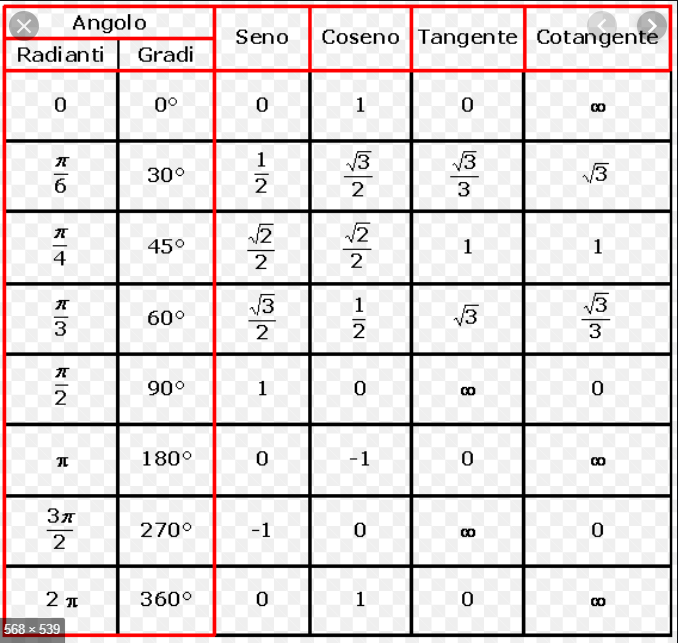
\includegraphics[width=300px]{../0-ripasso/trigonometria.PNG}
\end{figure}
\newpage
\subsection{Asintotici}
\begin{figure}[h!]
    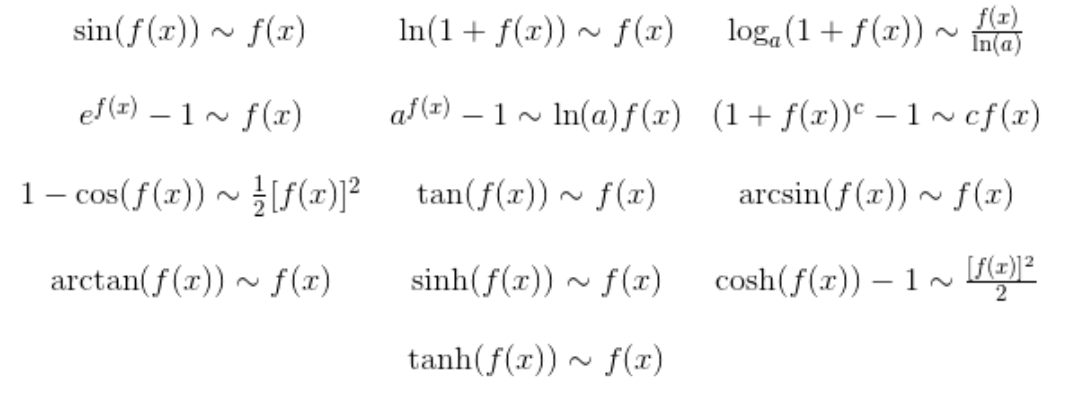
\includegraphics[width=\linewidth]{../0-ripasso/asintotici.PNG}
\end{figure}
\newpage
\subsection{Derivate}
\begin{figure}[h!]
    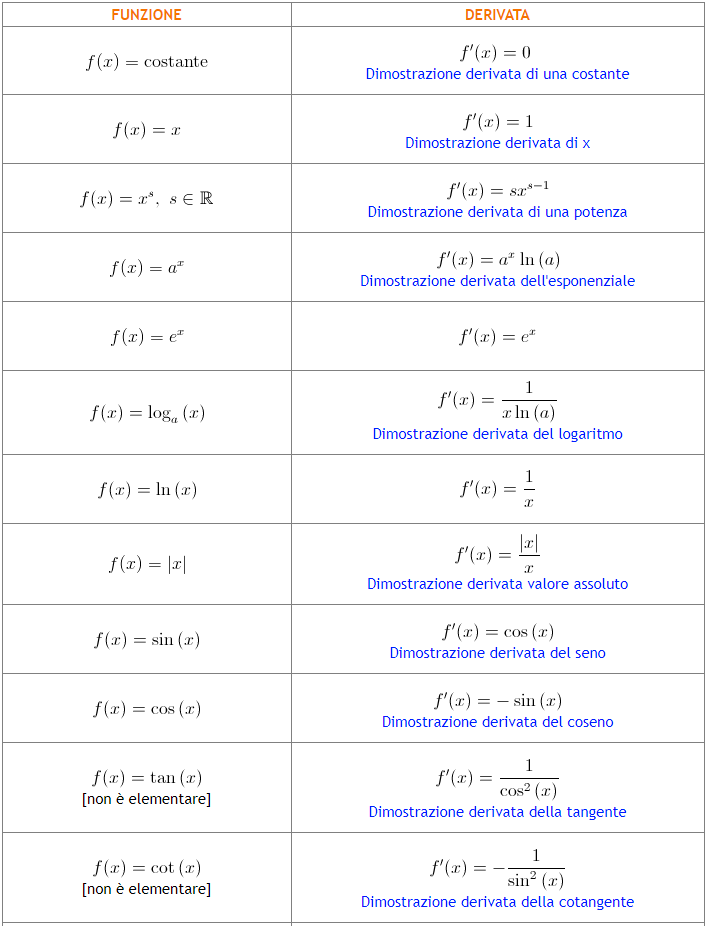
\includegraphics[width=\linewidth]{../0-ripasso/derivate1.PNG}
\end{figure}
\newpage
\begin{figure}[h!]
    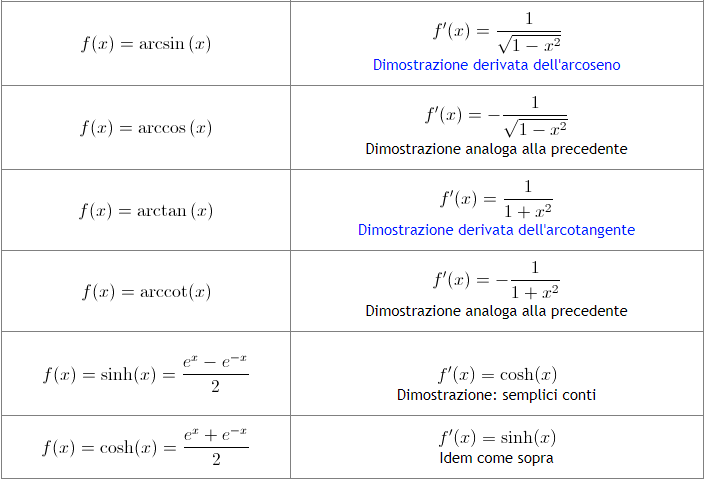
\includegraphics[width=\linewidth]{../0-ripasso/derivate2.PNG}
\end{figure}
\newpage
\subsection{Sviluppi}
\begin{figure}[h!]
    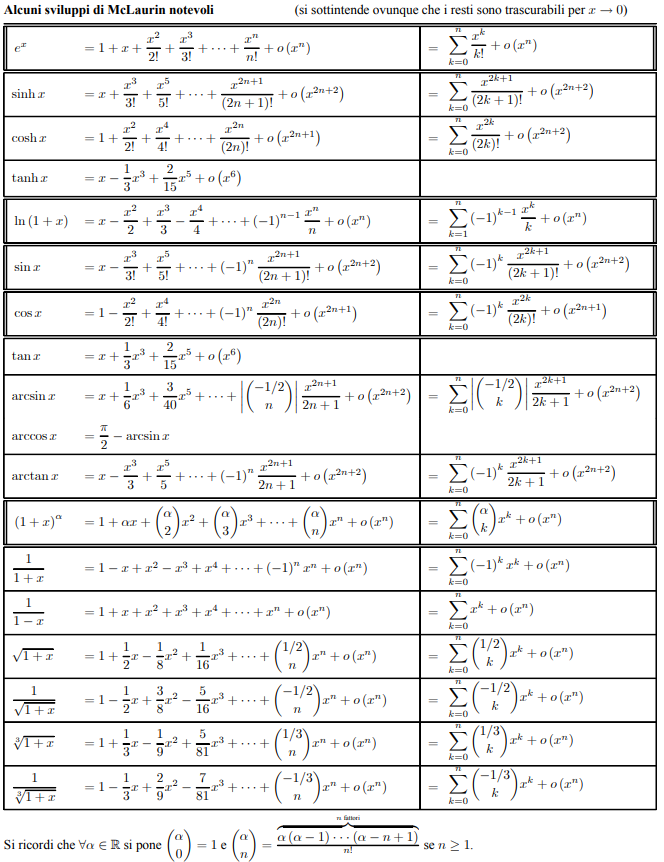
\includegraphics[width=\linewidth]{../0-ripasso/mclaurin.PNG}
\end{figure} % ripasso: trigonometria, derivate, asintotici, sviluppi di taylor da analisi I
    \newpage
    \section{Serie (analisi I)}
\subsection{Serie notevoli}
\subsubsection{serie geometrica}
\[
    \sum_{n=0}^{\infty}q^n = \lim_{k\rightarrow \infty} \frac{1-q^{k+1}}{1-q} = \begin{cases}
        \frac{1}{1-q} & se \;\; -1<q<1\\
        +\infty &se \;\; q \geq 1\\
        irregolare \;\;& se \;\; q\leq-1 
    \end{cases}
\]
\subsubsection{serie armonica}
\[
    \sum_{n=1}^{\infty}\frac{1}{n} \geq log(n+1) \rightarrow +\infty
\]
\subsubsection{serie armonica generalizzata}
\[
    \sum_{n=1}^{\infty} \frac{1}{n^{\alpha}}
\]
per $\alpha \leq 1$ 
\[
    \sum_{n=1}^{\infty} \frac{1}{n^\alpha} \geq \sum_{n=1}^{\infty}\frac{1}{n} \rightarrow +\infty \;\;\;\text{diverge}\;
\]
per $\alpha > 1$ 
\[
    \sum_{n=1}^{\infty} \frac{1}{n^\alpha} = converge
\]
per $\alpha = 2$
\[
    \sum_{n=1}^{\infty}\frac{1}{n^2} = \frac{\pi^2}{6} \left(\sim  \sum_{n=1}^{\infty} \frac{1}{n(n+1)} = serie \;\; di \;\; mengoli\right)
\]
\subsubsection{serie di mengoli}
\[
    \sum_{n=1}^{\infty}\frac{1}{n(n+1)} = \sum_{n=1}^{\infty} \frac{1}{n}-\frac{1}{n+1} = 1- \frac{1}{n+1} \rightarrow 1
\]
\subsubsection{numero e}
\[
    \lim_{n\rightarrow \infty} \left( 1 + \frac{1}{n} \right)^n = e
\]
\subsubsection{sviluppi di Taylor delle funzioni elementari}
\[
    e^x = \lim_{n\rightarrow +\infty}\sum_{k=0}^{n} \frac{x^k}{k!} = \sum_{k=0}^{+\infty} \frac{x^k}{k!}
\]
\[
    sin (x) =\sum_{k=0}^{\infty}(-1)^k \frac{x^{2k+1}}{(2k+1)!} =  \frac{e^{ix} - e^{-ix}}{2}
\]
\[
    cos (x) =\sum_{k=0}^{\infty}(-1)^k \frac{x^{2k}}{(2k)!} =\frac{e^{ix} + e^{-ix}}{2}
\]
\[
    Sh (x) = \sum_{k=0}^{\infty} \frac{x^{2k+1}}{(2k+1)!}
\]
\[
    Ch(x) = \sum_{k=0}^{\infty} \frac{x^{2k}}{(2k)!}
\]
\[
    log(1+x)= \sum_{k=1}^{\infty} (-1)^{k+1} \frac{x^k}{k} \;\;\; per \;\; |x|<1
\]
\[
    (1+x)^\alpha = \sum_{k=0}^{\infty} \binom{\alpha}{k}x^k \;\;\;\;\;\; \text{per $\alpha \in \mathbb{R}$ e per}\; |x|<1
\]
\subsection{Criteri e teoremi}
\textbf{teor.} Condizione necessaria affinché una serie $\sum_{n=0}^{\infty} a_n$ converga è che il termine generale $a_n$ tenda a zero. (Cioè perchè la serie converga, il termine $a_n$ deve tendere a zero, ma non per forza se il termine $a_n$ tende a zero allora la serie converge)\newline
\newline
\textbf{teor.}supponiamo che una serie $\sum_{n=0}^{\infty} a_n$ converga, allora per ogni $k$ anche risulta convergente anche $\sum_{n=k}^{\infty} a_n$.\newline
\newline
\textbf{Criterio serie a termini non negativi} Una serie $\sum_{n=0}^{\infty}a_n$ a termini non negativi è convergente o divergente a $+\infty$. Essa converge se e solo se la successione delle somme parziali n-esime è limitata.\newline
\newline
\textbf{Criterio del confronto} Siano $\sum an$ e $\sum b_n$ due serie a termini non negativi tali che $a_n<b_n$ definitivamente, allora:
\begin{itemize}
    \item $\sum b_n$ convergente $\Rightarrow \sum a_n$ convergente. 
    \item $\sum a_n$ divergente $\Rightarrow \sum b_n$ divergente. 
\end{itemize}
\textbf{Criterio del confronto asintotico} Se $a_n \sim b_n$, allora le corrispondenti serie $\sum a_n$ e $\sum b_n$ hanno lo stesso carattere (o entrambe divergenti o entrambe divergenti )\newline
\newline
\textbf{Criterio della radice} Sia $\sum a_n$ una serie a termini non negativi. Se esiste il limite 
\[
    \lim_{n\rightarrow +\infty}\sqrt[n]{a_n} = l
\]
\begin{itemize}
    \item $l>1$ la serie diverge $+\infty$
    \item $l<1$ la serie converge
    \item $l=1$ nulla si può concludere
\end{itemize}
Spesso utilizzato con termini che hanno come esponente $n$.\newline
\newline
\textbf{Criterio del rapporto} Sia $\sum a_n$ una serie a termini positivi. Se esiste il limite 
\[
    \lim_{n\rightarrow +\infty} \frac{a_{n+1}}{a_n} = l
\]
\begin{itemize}
    \item $l>1$ diverge $+\infty$
    \item $l<1$ converge 
    \item $l=1$ nulla si può concludere
\end{itemize}
Spesso utilizzato quando si hanno termini come $n^n$ e $n!$.\newline
\newline
\textbf{Criterio serie a termini di segno variabile} Una serie $\sum a_n$ si dice assolutamente convergente se converge la serie $\sum |a_n|$. Se la serie $\sum a_n$ converge assolutamente, allora converge.\newline
\newline
\textbf{Criterio di Leibniz} Sia data la serie 
\[
    \sum_{n=0}^{\infty}(-1)^n a_n \;\; con  \;\; a_n\geq 0 \;\forall\;n
\]
Se la successione $\{a_n\}$ è decrescente e se $a_n \rightarrow 0$ per $n \rightarrow \infty$, allora la serie è convergente.\newline
Il criterio di Leibniz può essere applicato anche se i termini sono definitivamente di segno alterno e la successione $a_n$ è definitivamente decrescente.\newline
Per verificare la decrescenza bisogna dimostrare che $a_{n+1}<a_n$ oppure mediante il limite a $+ \infty$ della derivata prima di $a_n$ o studiano quando la derivata prima di $a_n<0$ .\newline
Per determinare se una serie è decrescente non vanno usati gli asintotici !\newline
\newline
\textbf{Criterio della somma di serie convergenti} Se $\sum_{n=1}^{\infty} a_n$ converge e $\sum_{n=1}^{\infty} b_n$ converge, allora $\sum_{n=1}^{\infty} a_n +b_n$ converge.\newline
\newline
\textbf{Criterio della somma di serie convergenti e divergenti} Se $\sum_{n=1}^{\infty} a_n$ converge e $\sum_{n=1}^{\infty} b_n$ diverge, allora $\sum_{n=1}^{\infty} a_n + b_n$ diverge.\newline
\newline
\textbf{Criterio serie a termini complessi} Sia la serie $\sum_{n=0}^{\infty} a_n$ con $a_n$ complesso, se la serie  $\sum_{n=0}^{\infty} |a_n|$ converge, allora anche $\sum_{n=0}^{\infty} a_n$ converge \newline
\newline
\textbf{Criterio di Dirichlet} Siano $a_n$ e $b_n$ due succesioni tali che:
\begin{itemize}
    \item $a_n$ è a valori complessi e la sua successione delle somme parziali è limitata.
    \item $b_n$ è a valori reali positivi e tende monotonamente a zero
\end{itemize}
allora la serie $\sum a_nb_n$ è convergente.
    \newpage 
    \section{Serie di funzioni (analisi II)}
\subsection{Serie di potenze}
\subsubsection{Nel campo complesso}
\textbf{def.} Sia $\{a_n\}$ una successione di numeri complessi e sia $z_0 \in \mathbb{C}$.\newline
La serie
\[
    \sum_{n=0}^{\infty} a_n (z-z_0)^n
\]
si chiama \textbf{serie di potenza centrata} in $z_0$.\newline
\newline
Con la semplice traslazione $z-z_0 \rightarrow z$ possiamo ricondurci al caso $z_0 = 0$:
\[
    \sum_{n=0}^{\infty}a_n z^n
\]
\newline
Una serie di potenze ammette un $R \in [0, +\infty]$ tale che converge se $|z| < R$, non converge se $|z| > R$ e nulla si può dire se $|z| = R$.\newline
\newline
\textbf{Criterio del rapporto:} Se esiste
\[
    R = \lim_{n\rightarrow \infty}\left| \frac{a_n}{a_{n+1}}\right|
\]
allora la serie $\sum_{n=0}^{\infty}a_n z^n$ converge se $|z|< R$ e non converge se $|z|> R$.\newline
\newline
\textbf{Criterio della radice:} Se esiste
\[
    R = \lim_{n\rightarrow \infty} \frac{1}{\sqrt[n]{|a_n|}}
\]
allora la serie $\sum_{n=0}^{\infty}a_n z^n$ converge se $|z| < R$ e non converge se $|z|> R$.\newline
\newline
L'insieme di convergenza di una serie di potenze in $\mathbb{C}$ è un disco.\newline
Se $R = +\infty$ il disco è tutto $\mathbb{C}$, se $R = 0$ il disco è vuoto. Il numero $R \in [0, + \infty]$ si chiama \textbf{raggio di convergenza} della serie di potenza.\newline
\newline
Questi due criteri non dicono nulla sul comportamento della serie nei punti sul bordo del disco, cioè $|z| = R$.\newline
\newline
\textbf{teor.} Sia $\{a_n\}$ una successione di numeri complessi tale che la serie di potenze
\[
    f(z) = \sum_{n=0}^{\infty} a_n z^n
\]
converga per $|z|<R$ (con $R> 0$). Allora le serie ottenute derivando e integrando termine a termine, e cioè
\[
    \sum_{n=1}^{\infty} n a_n z^{n-1} \quad \quad \quad \sum_{n=0}^{\infty} \frac{a_n}{n+1} z^{n+1}
\]
sono rispettivamente la derivata e una primitiva della funzione $f$; inoltre, il loro raggio di convergenza è ancora $R$.\newline
\subsubsection{Nel campo reale}
Diremo che una serie di funzioni $\sum_{n}f_n(x)$ \textbf{converge puntualmente} per ogni $x \in I$ se la serie numerica $\sum_{n}f_n(x)$ converge per ogni $x \in I$.
\[
    f(x) = \sum_{n=0}^{\infty} f_n(x) = \lim_{k\rightarrow \infty} \sum_{n=0}^{k} f_n(x) \quad \;\forall\;x \in I
\]
cioè
\[
    f_n(x) \rightarrow f(x) \; \text{puntualmente se}\; \lim_{n\rightarrow \infty} f_n(x) = f(x) 
\]
\ \newline
Diremo che la serie di funzioni $\sum_{n}f_n(x)$ \textbf{converge uniformemente} a $f(x)$ su $I$ se
\[
    \lim_{k\rightarrow \infty} sup_{x \in I}\left| f(x) - \sum_{n=0}^{k}f_n(x) \right| = 0
\]
dove $f(x) = \sum_{n=1}^{\infty} f_n(x)$ è il limite puntuale della serie e $\sum_{n=0}^{k} f_n(x)$ è la somma parziale ennesima della serie.\newline
Cioè
\[
    f_n(x) \rightarrow f(x) \; \text{uniformemente se}\; \lim_{n\rightarrow \infty} sup_{x \in I}\left| f_n(x) - f(x) \right| = 0
\]
\ \newline
Diremo che la serie di funzioni $\sum_{n}f_n(x)$ \textbf{converge totalmente} su $I$ se
\[
    \sum_{n=0}^{\infty} sup_{x \in I}\left| f_n(x) \right| < + \infty
\]
\newline
\[
    \text{convergenza totale}\; \Longrightarrow \text{convergenza uniforme}\; \Longrightarrow \text{convergenza puntuale}
\]
\newline
Serie di potenza nel campo reale:
\[
    \sum_{n=0}^{\infty} a_n(x-x_0)^n
\]
che possiamo traslare nell'origine:
\[
    f(x) = \sum_{n=0}^{\infty} a_n x^n
\]
\newline
\textbf{Criteri del rapporto e della radice:} Si possono ancora usare i criteri della radice e del rapporto specificati nel campo complesso, $R$ rappresenta ancora il raggio del disco di convergenza nel piano complesso, ma essendo interessati all'asse reale si considera il solo intervallo $(-R, R)$.\newline
La serie di potenza nel campo reale converge \textbf{puntualmente} per ogni $x \in (-R, R)$, dove $R$ è dato dal criterio del rapporto o dal criterio della radice, e non converge se $|x| > R$.\newline
Come nel caso complesso, non possiamo dire nulle sulla convergenza in $x = \pm R$.\newline
Per quanto riguarda la convergenza \textbf{uniforme}, la serie di potenza nel campo reale converge uniformemente in $[-R+\epsilon, R- \epsilon]$ per ogni $\epsilon \in (0,R)$.\newline
\newline
\textbf{Criterio di Abel:} Se la serie di potenza $\sum_{n=0}^{\infty} a_n x^n$ converge per $x = R$, allora converge uniformemente in $[-R + \epsilon, R]$ per ogni $\epsilon \in (0,R)$; analogo risultato se la serie converge per $x = -R$. Se la serie converge per $x = \pm R$ allora converge uniformemente su tutto $[-R, R]$.\newline
\newline
\textbf{teor. (Integrazione per serie)}\newline
Se la serie di potenza $\sum_{n=0}^{\infty} a_n x^n$ converge uniformemente a $f$ su $[c,d]$ allora
\[
    \int_{c}^{d}f(x) dx = \int_{c}^{d}\left(\sum_{n=0}^{\infty}a_n x^n\right)dx = \sum_{n=0}^{\infty}a_n \int_{c}^{d}x^n dx = \sum_{n=0}^{\infty} a_n \frac{d^{n+1}- c^{n+1}}{n+1}
\]
\newline
\textbf{teor. (Derivazione per serie)}\newline
Date le serie
\[
    (1) \;\; \sum f_n(x) \quad \quad \quad \quad (2) \;\; \sum f_n'(x),
\]
se sono verificate le seguenti ipotesi:
\begin{itemize}
    \item le $f_n$ sono continue nell'intervallo $(a,b)$,
    \item la serie $(2)$ converge uniformemente in $(a,b)$,
    \item la serie $(1)$ converge per $x = x_0 \in (a,b)$  
\end{itemize}
allora valgono le seguenti tesi:
\begin{itemize}
    \item la serie $(1)$ converge uniformemente in $(a,b)$ (quindi converge a una funzione continua),
    \item la serie $(1)$ converge a una funzione derivabile in $(a,b)$,
    \item è possibile derivare la $(1)$ termine a termine, cioè
    \[
        \frac{d}{dx}\left(\sum f_n(x)\right) = \sum f_n'(x).
    \]
\end{itemize}
\subsubsection{Serie di Taylor / MacLaurin}
Introduciamo una vasta classe di funzioni elementari delle quali sappiamo scrivere esplicitamente le serie di potenza che le rappresentano.\newline
Data una funzione $f$ di classe $C^\infty$ in un punto $x_0$, possiamo scrivere formalmente
\[
    f(x) = \sum_{n=0}^{\infty} \frac{f^{(n)}(x_0)}{n!}(x-x_0)^n
\]
che, se poniamo $a_n = f^{(n)}(x_0)/n!$, coincide con una serie di potenza nel campo reale. Se $R > 0$ e la serie converge a $f$, allora la scrittura non è solo formale ma vale per ongi $x \in (x_0 - R, x_0 + R)$. In tale intervallo si ha convergenza puntuale, mentre la convergenza uniforme è garantita negli intervalli $[x_0 - R + \epsilon, x_0 + R -\epsilon]$ per ogni $\epsilon \in (0,R)$.
\[
    e^x = \sum_{n=0}^{\infty} \frac{x^n}{n!} \;\;\;\; (R= \infty)
\]
\[
    Ch(x) = \text{termini pari dello sviluppo di $e^x$}\;= \sum_{n=0}^{\infty} \frac{x^{2n}}{(2n)!} \;\;\;\; (R= \infty)
\]
\[
    Sh(x) = \text{termini dispari dello sviluppo di $e^x$}\;=  \sum_{n=0}^{\infty} \frac{x^{2n+1}}{(2n+1)!} \;\;\;\; (R= \infty)
\]
\[
    sin(x) = \sum_{n=0}^{\infty} \frac{(-1)^n}{(2n+1)!} x^{2n+1}\;\;\;\; (R= \infty)
\]
\[
    cos(x) = \sum_{n=0}^{\infty} \frac{(-1)^n}{(2n)!}x^{2n}\;\;\;\; (R= \infty)
\]
\[
    \frac{1}{1-x} = \sum_{n=0}^{\infty} x^n\;\;\;\; (R= 1)
\]
\[
    log(1+x) = \sum_{n=1}^{\infty} (-1)^{n+1} \frac{x^n}{n}\;\;\;\; (R= 1)\;\;\;\;\;\;\;\;\;\;\begin{cases}
        \text{se $x=1: $}\; \sum_{n=1}^{\infty}\frac{(-1)^{n+1}}{n} \;\;\text{(converge per Leibniz)}\;\\
        \text{se $x=-1$}\; \sum_{n=1}^{\infty}\frac{-1}{n} \;\;\text{(diverge, serie armonica)}\;
    \end{cases}
\]
\[
    \frac{1}{1+x^2} = \sum_{n=0}^{\infty} -1^n \cdot x^{2n} \;\;\;\;(R=1)
\]
\[
    arctan(x) = \sum_{n=0}^{\infty}(-1)^n \frac{x^{2n+1}}{2n+1} \;\;\;\;(R=1)
\]
\[
    (1+x)^\alpha = \sum_{n=0}^{\infty} \binom{\alpha}{n}x^n \;\;\;\; (R=1)
\]
\subsection{Serie di Fourier}
\subsubsection{Forma trigonometrica}
Nello studio delle serie di potenza $\sum_{n}a_n z^n$ abbiamo visto che i problemi principali riguardano lo studio di $|z| = R$ con $R$ raggio di convergenza. Per tali possiamo scrivere $z = R(cos(\theta) + sin(\theta))$ e ottenere:
\[
    \sum_{n=0}^{\infty} a_n R^n(cos(n \theta) + isin(n \theta))
\]
Se $\{a_n\} \subset \mathbb{R}$, siamo quindi portati a studiare la convergenza di serie trigonometriche del tipo
\[
    \sum_{n=0}^{\infty} \alpha_n cos(n \theta) \;\;\;\;\; \;\;\;\;\; \sum_{n=1}^{\infty} \beta_n sin(n \theta)
\]
Per ogni scelta di $\alpha_n, \beta_n \in \mathbb{R}$ le funzioni
\[
    a_0 + \sum_{n=1}^{\infty} (\alpha_n cos(nx) + \beta_n sin(n x))
\]
si chiamano \textbf{polinomi trigonometrici} di grado $k$; che sono funzioni periodiche di periodo $2\pi$ che hanno valor medio $\alpha_0$ su $[0, 2\pi]$.\newline
Diremo che una serie in forma trigonometrica converge se converge una successione di polinomi trogonometrici.\newline
\textbf{oss.} 
\[
    \sum_{n=1}^{\infty} (|\alpha_n| + |\beta_n|) < \infty \Rightarrow \text{converge totalmente su } [0,2\pi] \Rightarrow \text{converge uniformemente} \Rightarrow \text{converge puntualmente}
\]
\textbf{oss.} La serie trigonometrica può perdere la convergenza dopo una derivazione.\newline
\newline
\textbf{Criterio di Dirichlet}
\[
    \alpha_n, \beta_n \downarrow 0 \Rightarrow \text{polinomio trigonometrico converge puntualmente su} (0,2\pi)
\]
dove con il simbolo $\downarrow 0$ indichiamo che le successioni descrescono monotonamente a $0$ e che sono positive.\newline
\newline
\textbf{Lemma.} Per ogni $m,n = 1,2,\dots$ risulta 
\[
    \int_{0}^{2\pi} sin(nx) dx = \int_{0}^{2\pi} cos(nx) = 0
\]
\[
    \int_{0}^{2\pi} sin(mx) cos(nx) dx = 0
\]
\[
    \int_{0}^{2\pi} sin^2(nx) dx = \int_{0}^{2\pi} cos^2(nx) dx = \pi
\]
\[
    \int_{0}^{2\pi} sin(mx) sin(nx) dx = \int_{0}^{2\pi} cos(mx) sin(nx) dx = 0 \;\;\;\; \text{se} \; m\neq n
\]
Si trovano gli stessi valori integrando su qualunque intervallo di ampiezza $2\pi$.\newline
\newline
\textbf{teor. calcolo delle serie di Fourier per funzioni $2\pi$-periodiche} 
Se una funzione $f$ è $2\pi$-periodica ed è sviluppabile in serie di Fourier, si ha che
\[
    f(x) \sim  \frac{a_0}{2} + \sum_{n=1}^{\infty}(a_n cos(nx) + b_n sin(nx))
\]
allora
\[
    a_n = \frac{1}{\pi} \int_{I} f(x) cos(nx) dx \;\;\;\; \;\forall\;n\geq0
\]
\[
    b_n = \frac{1}{\pi} \int_{I} f(x) sin(nx) dx \;\;\;\;\;\forall\;n\geq 1
\]
dove l'intervallo $I$ è un qualunque intervallo di ampiezza $2\pi$ (tipicamente si prende da $-\pi$ a $\pi$, per sfruttare eventuali simmetrie\dots) e il termine $a_0$ si calcola come $a_0 = \frac{1}{\pi} \int_{I} f(x) dx$.\newline
Gli $a_n$ e $b_n$ vengono chiamati \textbf{coefficienti di Fourier} di $f$, mentre la serie $f(x) = \frac{a_0}{2} + \sum_{n=1}^{\infty}(a_n cos(nx) + b_n sin(nx))$ viene chiamata \textbf{serie di Fourier} associata a $f$.\newline
\newline
\textbf{oss.} Gli integrali del teorema si possono calcolare se risulta $\int_{0}^{2\pi}|f| < \infty$ e cioè se l'integrale improprio di $|f|$ è convergente.\newline
\newline
Diremo che la serie 
\[
    f(x) = \frac{a_0}{2} + \sum_{n=1}^{\infty}(a_n cos(nx) + b_n sin(nx))
\]
\textbf{converge in media quadratica} alla $f$ se
\[
    \lim_{k\rightarrow \infty} \int_{0}^{2\pi} \left| f(x) - \frac{a_0}{2} - \sum_{n=1}^{k}\left( a_n cos(nx) + b_n sin(nx) \right) \right|^2 dx = 0
\]
\newline
\textbf{teor.} Sia $f$ una funzione $2\pi$-periodica tale che $\int_{0}^{2\pi}f^2 < \infty$. Allora la sua serie di Fourier converge a $f$ in media quadratica.\newline
\newline
Definiamo lo spazio $X$ delle funzioni $f$ tali che $\int_{0}^{2\pi}f^2 < \infty$ e introduciamo il "prodotto scalare" definito come
\[
    (x,g)_{X} = \frac{1}{\pi}\int_{0}^{2\pi} f(x) g(x) dx \;\;\;\;\; \;\forall\;f,g \in X
\]
per cui troviamo che 
\[
    B = \left\{ \frac{1}{\sqrt{2}}, cos(nx), sin(nx) \right\}_{n=1} ^\infty
\]
è ortonormale in $X$.\newline
\newline
\textbf{teor. Identità di Parseval}\newline
Sia $f \in X$ e sia $f(x) = \frac{a_0}{2} + \sum_{n=1}^{\infty}(a_n cos(nx) + b_n sin(nx))$ la sua serie di Fourier. Allora
\[
    \frac{1}{\pi} \int_{0}^{2\pi} f(x)^2 dx = \frac{a_0^2}{2} + \sum_{n=1}^{\infty}(a_n^2 + b_n^2)
\]
Per il teorema di Riemann-Lebesgue sappiamo che $a_n, b_n \rightarrow  0$ per $n \rightarrow  \infty$.\newline
\newline
\[
\text{convergenza uniforme}\; \Rightarrow \text{convergenza in media quadratica}\; \Rightarrow 
\]
\[
    \Rightarrow  \text{convergenza puntuale su sottosuccession in quasi ogni punto}\;
\]
\newline
\textbf{def.} Diciamo che $f : [0,2\pi] \rightarrow \mathbb{R}$ è \textbf{regolare a tratti} se è limitata in $[0,2\pi]$ e se l'intervallo $[0,2\pi]$ si può scomporre in un numero finito di sottointervalli su ciascuno dei quali $f$ è continua e derivabile; inoltre, agli estremi di ogni sottointervallo, esistno finiti i limiti sia di $f$ che di $f'$.\newline
\newline
\textbf{oss.} se $f \in C^1[0,2\pi]$ allora $f$ è regolare a tratti. Ma anche se ci sono punti angolosi o punti di discontinuità a salto, purchè $f$ e $f'$ abbiano limiti finiti in prossimità dei salti, allora $f$ è regolare a tratti. Non devono esserti asintoti verticali o punti a tangenza verticale.\newline
\newline
Se una funzione $f$ è regolare a tratti allora la sua serie di Fourier converge a $f$ in media quadratica. Dunque a meno di pochi possibili punti, la conergenza sarà anche puntuale.\newline
\newline
\textbf{teor.} Sia $f: [0,2\pi] \rightarrow \mathbb{R}$ regolare a tratti. Allora la sua serie di Fourier converge in ogni punto $x_0 \in [0,2\pi]$ alla media dei due limiti $f(x_0^{\pm})$:
\[
    \frac{a_0}{2} + \sum_{n=1}^{\infty} \left( a_n cos(nx_0) + b_n sin(nx_0) \right) = \frac{f(x_0^+) + f(x_0^-)}{2}
\]
con la convenzione che $f(0^\pm) = f(2\pi^\pm)$. In particolare, se $f$ è continua in $x_0$, allora la serie converge a $f(x_0)$.
\subsubsection{Funzioni con periodi diversi da $2\pi$}
Come ci si comporta in presenza di funzioni con periodo $T \neq 2\pi$?\newline
L'unica differenza sta nel calcolo dei coefficienti di Fouriere:
\[
    a_n = \frac{2}{T}\int_{0}^{T}f(x) cos\left( \frac{2\pi n}{T}x \right) dx, \;\;\;\;\; \;\;\;\;\; b_n = \frac{2}{T} \int_{0}^{T}f(x) sin\left( \frac{2\pi n}{T}x \right)
\]
La funzione $f$ si scrive allora:
\[
    f(x) = \frac{a_0}{2} + \sum_{n=1}^{\infty} \left( a_n cos\left( \frac{2\pi n}{T}x \right) + b_n sin \left( \frac{2\pi n}{2}x \right) \right)
\]
Tutti i teoremi valgono allo stesso modo, l'unico da "sistemare" è l'identità di Parseval, che, per fuznioni $T$-periodiche $f$ soddisfacenti $\int_{0}^{T} f^2 < \infty$, diventa:
\[
    \frac{2}{T} \int_{0}^{T}f(x)^2 dx = \frac{a_0^2}{2} + \sum_{n=1}^{\infty} (a_n^2 + b_n^2)
\]
\subsubsection{Forma esponenziale complessa}
La formula di Eulero, $e^{i \theta} = cos(\theta) + i sin(\theta)$, suggerisce di scrivere una serie di Fourier utilizzando gli esponenziali.
\[
    f_n =\frac{a_n-ib_n}{2} = \frac{1}{2\pi} \int_{0}^{2\pi}f(x)(cos(nx) - i sin(nx))dx = \frac{1}{2\pi} \int_{0}^{2\pi}f(x) e^{-inx}
\]
\[
    f_{-n} =\frac{a_n + ib_n}{2} = \frac{1}{2\pi} \int_{0}^{2\pi}f(x)(cos(nx) + i sin(nx))dx = \frac{1}{2\pi} \int_{0}^{2\pi}f(x) e^{inx}
\]
da cui
\[
    a_n = f_n + f_{-n}
\]
\[
    b_n = i (f_n)
\]
\[
    f(x) = \frac{a_0}{2} + \sum_{n=1}^{\infty} \left( a_n cos(nx) + b_n sin(nx) \right) = \sum_{n=-\infty}^{\infty} f_n e^{inx}
\]
\newline
Identità di Parseval:
\[
    \frac{1}{2\pi}\int_{0}^{2\pi}f(x)^2dx = \sum_{n=-\infty}^{\infty}|f_n|^2
\]
\subsection{Note sugli esercizi}
\subsubsection{Serie di potenze nel campo reale}
Sono dette serie di potenza le serie di funzioni della forma:
\[
    \sum_{n} a_nx^n \;\;\;\;\;\;\;\;\;\;\;\;\;\;\;\sum_{n}a_n(x-x_0)^n
\]
in cui la prima si dice centrata nell'origine e la seconda centrata in $x_0$ (con la semplice traslazione di $x-x_0$ a $x$ ci si può sempre ricondurre al caso $x_0 = 0$).\newline
\newline
Una volta calcolato il raggio di convergenza $R$ come
\[
    R = \lim_{n\rightarrow +\infty} \frac{|a_n|}{|a_{n+1}|} \;\;\;\;\;\;\;\;\;\;\;\;\;\;\;R = \lim_{n\rightarrow +\infty} \frac{1}{\sqrt[n]{|a_n|}}
\] dove l'uso della prima o della seconda è suggerito dalle circostanze, ci sono tre casi possibili:
\begin{itemize}
    \item $R = 0$, la serie converge se e solo se $x = x_0$;
    \item $R = +\infty$, la serie converge puntualmente per ogni $x \in \mathbb{R}$;
    \item $0 < R < \infty$, \begin{itemize}
        \item la serie converge puntualmente se $|x-x_0| < R$, ossia nell'intervalo $(x_0-R, x_0 + R)$
        \item la serie non converge se $|x-x_0| > R$
        \item nulla si può dire riguardo al comportamento della serie nei punti $x = x_0 - R$ e $x= x_0+R$
    \end{itemize}
\end{itemize}
Per calcolare il raggio di convergenza $R$ si usano due formule:
\[
    R = \lim_{n\rightarrow +\infty} \frac{|a_n|}{|a_{n+1}|}
\]
\[
    R = \lim_{n\rightarrow +\infty} \frac{1}{\sqrt[n]{|a_n|}}
\]
\subsubsection{Convergenza uniforme per serie di potenza}
Se una serie di potenze converge per $x \in (a,b)$, si dimostra che tale serie converge uniformemente in ogni intervallo $[\alpha, \beta]$ con $a < \alpha< \beta < b$.\newline
\newline
Vale inoltre il \textbf{teorema di Abel}: se la serie di potenze $\sum a_n (x-x_0)^n$, converge negli estremi di un intervallo $[a,b]$, allora converge uniformemente in tutto l'intervallo $[a,b]$.\newline
\newline
Possibili casi:
\begin{itemize}
    \item converge in $x \in[a,b]$, converge uniformemente in $[a, b]$
    \item converge in $x \in[a,b)$, fissato un $\epsilon > 0$, converge uniformemente in $[a, b-\epsilon]$
    \item converge in $x \in(a,b]$, fissato un $\epsilon > 0$, converge uniformemente in $[a + \epsilon, b]$
    \item converge in $(a,b)$, fissato un $\epsilon > 0$ e $\delta > 0$, converge uniformemente in $[a + \delta, b-\epsilon]$
    \item converge per $x$ uguale a un solo punto, non ha senso parlare di convergenza uniforme
    \item converge per $x \in\mathbb{R}$, converge uniformemente in $[\alpha, \beta]$ con $-\infty < \alpha < \beta < + \infty$
\end{itemize}
\subsubsection{Sviuluppabilità in serie di Fourier}
Una funzione periodica $f: \mathbb{R} \rightarrow  \mathbb{R}$ è sviluppabile in serie di Fourier se vale una delle due condizioni seguenti:
\begin{itemize}
    \item $f$ è limitata e monotona a tratti su un periodo, oppure
    \item il quadrato di $f$ è integrabile su un periodo (vale meno di $\infty$).
\end{itemize}
Inoltre se la funzione $f$ è continua in $x_0$, allora la serie di Fourier converge al valore della funzione, viceversa se in $x_0$ è presente una discontinuità di prima specie (ma $f$ è limitata e monotona a tratti):
\[
    \lim_{x\rightarrow x_0^-} f(x) = f_-(x_0)
\]
\[
    \lim_{x\rightarrow x_0^+} f(x) = f_+(x_0)
\]
\[
    f_-(x_0) \neq f_+(x_0)
\]
allora (quale sia il valore che $f$ assume in $x_0$) il valore della serie in $x_0$ è la media aritmentica dei due valori:
\[
    \frac{f_-(x_0) + f_+(x_0)}{2}
\]
\newline
In parole povere, \textbf{per valutare se la funzione sia rappresentabile o meno con una serie di Fourier}, per prima cosa si controlla se è limitata e monotona tratti su un periodo (si capisce con una analisi grafica), se lo è allora la funzione è rappresentabile con Fourier. Altrimenti si può usare anche un metodo analitico: si prende la funzione, e si fa l'integrale $\int_{0}^{2\pi} f^2$, se l'integrale ha un valore finito, allora la funzione può essere sviluppata con una serie di Fourier. Da notare che l'integrale può essere svolto anche in senso generalizzato per risolvere puntii in cui la funzione va a $\infty$.\newline
\textbf{Per valutare per quali valori di $x$ la serie converge effettivamente alla funzione indicata}, si usa il seguente criterio: dove la funzione è continua, la serie converge al valore della funzione, dove ci sono discontinuità a salto la serie converge al valor medio degli estremi del salto, dove ci sono altri tipi di discontinuità non si può concludere nulla sul comportamento della seria.
\subsubsection{Calcolo delle serie di Fourier per funzioni $2\pi$-periodiche} 
Se una funzione $f$ è $2\pi$-periodica ed è sviluppabile in serie di Fourier, si ha che
\[
    f(x) \sim  \frac{a_0}{2} + \sum_{n=1}^{\infty}(a_n cos(nx) + b_n sin(nx))
\]
allora
\[
    a_n = \frac{1}{\pi} \int_{I} f(x) cos(nx) dx \;\;\;\; \;\forall\;n\geq0
\]
\[
    b_n = \frac{1}{\pi} \int_{I} f(x) sin(nx) dx \;\;\;\;\;\forall\;n\geq 1
\]
dove l'intervallo $I$ è un qualunque intervallo di ampiezza $2\pi$ (tipicamente si prende da $-\pi$ a $\pi$, per sfruttare eventuali simmetrie\dots) e il termine $a_0$ si calcola come $a_0 = \frac{1}{\pi} \int_{I} f(x) dx$.
\subsubsection{Semplificazioni nel calcolo delle serie di Fourier per funzioni pari e dispari}
I coefficienti di Fourier di funzioni $2\pi$-periodiche si possono calcolare integrando su un qualunque intervallo di ampiezza $2\pi$. Tipicamente si sceglie l'intervallo $[-\pi, \pi]$ perchè permette di sfruttare eventuali simmetrie della funzione $f$.\newline
Infatti, se la funzione $f$ è \textbf{pari} allora risulta pari anche $f(x)cos(nx)$ mentre risulta dispari $f(x)sin(nx)$, dunque:
\[
    f \; \text{pari}\; \Rightarrow a_n = \frac{2}{\pi} \int_{0}^{\pi}f(x) cos(nx) dx , \;\;\;\;\;b_n = 0
\]
Invece, se la funzione $f$ è \textbf{dispari} allora risulta dispari anche la funzioen $f(x)cos(nx)$ mentre risulta pari $f(x) sin(nx)$, dunque:
\[
    f \; \text{dispari}\; \Rightarrow a_n = 0, \;\;\;\;\;b_n = \frac{2}{\pi} \int_{0}^{\pi} f(x) sin(nx)dx
\]
\subsubsection{Riassunto dei criteri per la convergenza della serie di Fourier $\sum F$}
\textbf{Appunti prof:}\newline
Condizione di partenza:
\[
    \int_{0}^{2\pi}f^2 < \infty \Leftrightarrow \text{possiamo calcolare}\;\{a_n, b_n\}
\]
\begin{itemize}
    \item se $\sum_{n=1}^{\infty}(|a_n| + |b_n|) < \infty$ (converge) $\Rightarrow \sum F \rightarrow f$ totalmente $\Rightarrow \sum F \rightarrow  f$ uniformemente.\newline
    Proprietà: una successione/serie di funzioni continue che converge uniformemente ha limite continuo.
    \item se $f$ non è continua, la serie di Fourier $\sum F$ non può convergere uniformemente.
    \item $\int_{0}^{2\pi}f^2 < \infty $ e cioè $\sum_{n=0}^{\infty}(a_n^2 + b_n^2)< \infty \;\;\Longleftrightarrow \;\;\sum F \rightarrow f$ in media quadratica.
    \item Criterio di Dirichlet: se $a_n, b_n \downarrow 0 \Rightarrow  \sum F \rightarrow f$ puntualmente su $(0,2\pi)$.
    \item $f$ regolare a tratti $\Rightarrow \sum F(x) \rightarrow  \frac{f(x)^+ + f(x)^-}{2}$ puntualmente su $[0,2\pi]$
\end{itemize}
\textbf{Note dal libro di esercizi:}\newline
Data la generica funzione di Fourier:
\[
    f(x) \sim  \frac{a_0}{2} + \sum_{n=1}^{\infty} a_n cos(nx) + b_n sin(nx)
\]
per stabilirne la convergenza è possibile percorrere due strade:
\begin{itemize}
    \item Criterio di Dirichlet: se le successioni $a_n$ e $b_n$ sono monotone decrescenti e tendono a $0$, allora la serie di Fourier covnerge in tutti i punti, tranne al più in $x = 2k\pi$.
    \item Criterio di Weierstrass per le serie di funzioni: Data una serie di funzioni $\sum f_n(x)$, se per $x \in [a,b]$ si ha che
    \begin{itemize}
        \item $|f_n(x)| \leq c_n$
        \item $\sum c_n$ converge
    \end{itemize}
    allora la serie di partenza converge uniformemente in tutto l'intervallo $[a,b]$.\newline
    Per usarlo con le serie di Fourier: poichè
    \[
        |a_n cos(nx) + b_n sin(nx)| \leq |a_n| + |b_n|
    \]
    se la serie $\sum |a_n| + |b_n|$ converge, allora la serie di Fourier converge (uniformemente), e quindi la funzione a cui converge è continua.
\end{itemize}
Inoltre, poichè derivando la funzione termine a termine, otteniamo la serie
\[
    \sum_{n=1}^{\infty} (n b_n ) cos(nx) - (n a_n)sin(nx)
\]
è sufficiente riapplicare a qeust'ultima i criteri di convergenza, per controllare se la serie di partenza converge a una funzione derivabile.
\subsubsection{Armoniche}
\[
    f(x) \sim \text{valor medio}\; + \sum_{n=1}^{\infty}\alpha_n cos(nx + \theta_n)
\]
dove
\[
    \alpha_n = \sqrt{a_n^2 + b_n^2}
\]
e
\[
    cos(\theta_n) = \frac{a_n}{\sqrt{a_n^2 + b_n^2}}
\]
\[
    sin(\theta_n) = -\frac{b_n}{\sqrt{a_n^2 + b_n^2}}
\]
da cui si ricava che $\theta_n$ è:
\[
    \theta_n = \begin{cases}
        arctan\left(\frac{-b_n}{a_n}\right) \;\;\;\; &se \; a_n > 0\\
        \pi + arctan\left(\frac{-b_n}{a_n}\right) \;\;\;\;& se \; a_n < 0
    \end{cases}
\]
se $a_n = 0$, non si può usare l'arcotangente, ma in tal caso la trasposizione diventa:
\[
    b_n sin(nx) = b_n cos(nx - \frac{\pi}{2})
\]
    \newpage
    \section{Funzioni $R \rightarrow R^n$ ("Funzioni di una variabile a valori vettoriali", "Curve nel piano e nello spazio")}
\subsection{Introduzione alle funzioni $R \rightarrow R^n$}
\subsubsection{Definizioni e terminologia}
Si dice \textbf{funzione a valori vettoriali} una funzione $\vec{f} : \mathbb{R} \rightarrow  \mathbb{R}^n$ con $n > 1$.\newline
\newline
Il \textbf{limite} della funzione a valori vettoriali si calcola componente per componente:
\[
    \lim_{t\rightarrow t_0}(r_1(t), r_2(t), \dots, r_n(t)) = \left(\lim_{t\rightarrow t_0}r_1(t), \lim_{t\rightarrow t_0}r_2(t), \dots, \lim_{t\rightarrow t_0}r_n(t)\right)
\]
Valgono allo stesso modo delle funzioni unidimensionali il teorema di unicità del limite e la definizione di \textbf{continuità} (una funzione a valori vettoriali è continua in un punto se lo sono tutte le sue componenti).\newline
\newline
Nel caso $n = 2$ o $3$, una funzione $\vec{f} : \mathbb{R} \rightarrow  \mathbb{R}^n$ rappresenta una curva nel piano o nello spazio tridimensionale.\newline
\newline
Sia $I$ un intervallo in $\mathbb{R}$. Si dice \textbf{arco di curva continua}, o \textbf{cammino}, in $\mathbb{R}^n$ una funzione $\vec{r}: I \rightarrow \mathbb{R}^n$ continua.\newline
\newline
Una curva si dice \textbf{chiusa} se $\vec{r}(a) = \vec{r}(b)$ con $I=[a,b]$.\newline
\newline
Una curva si dice \textbf{semplice} se non ripassa mai nello stesso punto, cioè se $r:(a,b) \rightarrow \mathbb{R}^n$ è iniettiva..\newline
\newline
Una curva si dice \textbf{piana} se esiste un piano che contiene il suo sostegno (in particolare tutte le curve  $f: \mathbb{R} \rightarrow \mathbb{R}^n$ con $n=2$).\newline
\newline
Il \textbf{sostegno} della curva è l'immagine della funzione, cioè l'insieme dei punti di $\mathbb{R}^n$ percorsi dal punto mobile.\newline
\newline
Due curve si dicono \textbf{equivalenti} se hanno lo stesso sostegno.
\subsubsection{Calcolo differenziale per funzioni $R \rightarrow R^n$}
Sia $\vec{r}: I \rightarrow \mathbb{R}^n$ e $t_0 \in I$, si dice che $\vec{r}$ è \textbf{derivabile} in $t_0$ se esiste finito
\[
    \vec{r}'(t_0) = \lim_{h\rightarrow 0}\frac{\vec{r}(t_0 +h) - \vec{r}(t_0)}{h}
\]
Se $\vec{r}$ è derivabile in tutto $I$ e inoltre $\vec{r}'$ è continuo in $I$, si dice che $\vec{r}$ è di \textbf{classe} $C^1(I)$ ($\vec{r}\in C^1(I)$).
\newline
\newline
Notiamo che il \textbf{vettore derivato} è il \textbf{vettore delle derivate} delle componeneti:
\[
    \vec{r'}(t_0) = (r'_1(t_0), r'_2(t_0), \dots, r'_n(t_0))
\]
\ \newline
Sia $I \subseteq \mathbb{R}$ un intervallo. Si dice arco di curva \textbf{regolare} un arco di curva $\vec{r}: I \rightarrow  \mathbb{R}^n$ tale che $\vec{r} \in C^1(I)$ e $\vec{r}'(t) \neq 0$ per ogni $t \in I$ (solo nell'intervallo aperto, queste due proprietà possono non verificarsi agli estremi).\newline
Il fatto che $\vec{r}' (t) \neq 0$ è una proprietà il cui significato è vettoriale: le componenti di $\vec{r}'(t)$ non possono annullarsi contemporanemante, e cioè che $|\vec{r}'(t)|\neq 0$, cioè che il punto mobile non si ferma mai ($\vec{r}'(t)$ rappresenta la velocità).\newline
\newline
Dato un vettore $\vec{r}(t)$ si dice
\begin{itemize}
    \item \textbf{velocità}: $\vec{r}'(t)$
    \item \textbf{velocità scalare}: $|\vec{r}'(t)|$
    \item \textbf{accellerazione}: $\vec{r}''(t)$
    \item \textbf{accellerazione scalare}: $|\vec{r}''(t)|$
\end{itemize}
\ \newline
Di conseguenza per le curve regolari è ben definito il \textbf{versore tangente}:
\[
    \vec{T} = \frac{\vec{r}'(t)}{|\vec{r}'(t)|}
\]
\ \newline
Si dice arco di curva \textbf{regolare a tratti} un arco di curva $\vec{r} : I \rightarrow \mathbb{R}^n$ tale che: $\vec{r}$ è continua e l'intervallo $I$ può essere suddiviso in un numero finito di sottointervalli, su ciascuno dei quali $\vec{r}$ è un arco di curva regolare.\newline
\newline
Alcune \textbf{proprietà} del calcolo differenziale vettoriale:
\[
    (\vec{u} + \vec{v})' = \vec{u}' + \vec{v}'
\]
\[
    (c \vec{u})' = c \vec{u}' \;\;\; \text{con c costante}
\]
\[
    (f \vec{u})' = f' \vec{u} + \vec{u}' f \;\;\;\text{con} \; f \; \text{funzione}
\]
\[
    [\vec{u}(f(t))]' = \vec{u}'(f(t))f'(t)
\]
\[
    (\vec{u} \cdot \vec{v})' = \vec{u}' \cdot  \vec{v} + \vec{u} \cdot  \vec{v}'
\]
\[
    (\vec{u} \text{x} \vec{v})' = \vec{u}' \text{x} \vec{v} + \vec{u} \text{x} \vec{v}' \;\;\; in \;\mathbb{R}^3
\]
\subsubsection{Calcolo integrale per funzioni $R \rightarrow R^n$}
\[
    \int_{a}^{b} \vec{r}(t) dt =\left( \int_{a}^{b}\vec{r_1}(t) dt,\int_{a}^{b}\vec{r_2}(t) dt, \dots, \int_{a}^{b}\vec{r_n}(t) dt,\right)
\]
Diremo che $\vec{r}$ è \textbf{integrabile} in $[a,b]$ se lo è ognuna delle sue componenti.\newline
\[
    \int_{a}^{b} \vec{r}'(t) dt = \vec{r}(b) - \vec{r}(a)
\]
Può essere utile utilizzare il seguente lemma:
\[
    \left| \int_{a}^{b}\vec{r}(t)dt \right| \leq \int_{a}^{b}|\vec{r}(t)|dt
\]
Se $\vec{r}(t)$ è una curva regolare e chiusa in $[a,b]$, allora $\int_{a}^{b}\vec{r}'(t) dt =0$.
\subsection{Lunghezza di un arco di curva}
\subsubsection{Curve rettificabili e lunghezza}
Si dice che $\gamma$ è \textbf{rettificabile} se 
\[
    sub_\mathcal{P} l(\mathcal{P}) = l(\gamma) < + \infty
\]
Dove l'estremo superiore è calcolato al variare di tutte le possibili partizioni $\mathcal{P}$ di $[a,b]$.\newline
In tal caso $l(\gamma)$ assegna per definizione, la lunghezza di $\gamma$.\newline
\newline
\textbf{teor.} Sia $\vec{r}:[a,b] \rightarrow \mathbb{R}^n$ la parametrizzazione di un arco di curva $\gamma$ regolare. Allora $\gamma$ è rettificabile e la sua \textbf{lunghezza} vale 
\[
    l(\gamma) = \int_{a}^{b}|\vec{r}'(t)| dt
\]
Nello spazio tridimensionale la formula diventa:
\[
    l(\gamma)= \int_{a}^{b}\sqrt{x'(t)^2 + y'(t)^2 + z'(t)^2}dt
\]
(Da un punto di vista fisico queste due formule ci dicono che lo spostamento è l'integrale della velocità, cosa ben nota).
\ \newline
Inoltre:\newline
Sia $\gamma$ l'unione di due curve rettificabili, allora $\gamma$ è rettificabile, la stessa proprietà si estende a un numero finito qualsiasi di curve rettificabili. \newline
Se una curva $\gamma$ è regolare a tratti, allora è rettificabile.\newline
\newline
Vediamo il caso in si vuole calcolare la \textbf{lunghezza di un grafico di una funzione} $f(x)$:\newline
Sia $\gamma$ una curva piana regolare che sia grafico di una funzione, ossia:
\[
    \gamma : \begin{cases}
        x =t \\
        y= f(t)
    \end{cases} \;\; \text{per} \;t \in[a,b]
\]
allora
\[
    l(\gamma) = \int_{a}^{b}\sqrt{1+f'(t)^2}dt
\]
\subsubsection{Riparametrizzazioni e parametro arco (o ascissa curvilinea)}
Sostanzialmente, due curve equivalenti dipendono da un cambio di variabile. Se $r = r(t)$ con $t \in[a,b]$ ha per sostegno $\gamma$ e se $\phi: [c,d] \rightarrow [a,b]$ è una funzione continua e strettamente monotona (crescente o descrescente), allora la curva $\rho(t) := r(\phi(t))$, con $t \in [c,d]$, ha lo stesso sostegno di $\gamma$. Si usa dire che $\rho(t)$ è una \textbf{riparametrizzazione} di $r(t)$.\newline
Notiamo che dopo una riparametrizzazione la lunghezza dell'arco di curva rimane la stessa, anche se il verso o la velocità di percorrenza cambiano (es. per invertire il senso di percorrenza si può riparametrizzare $t$ con $-t$).\newline
\newline
Se invece di calcolare la lunghezza di una curva da un valore $a$ a un valore $b$, cioè in $[a,b]$, la calcolassimo in $[t_0, t]$, con $t_0$ un effettivo valore e $t$ una variabile, otterremmo una funzione di $t$ definita come:
\[
    s(t) = \int_{t_0}^{t}|\vec{r}'(\tau)|d\tau
\]
Inoltre se si è in grado di calcolare esplicitamente tale funzione e poi di invertirla, esprimendo $t$ come funzione di $s$, è possibile riparametrizzare la curva in funzione del parametro $s$, detto \textbf{parametro arco} o \textbf{ascissa curvilinea} (ricordarsi di ricalcolare anche gli estremi dell'intervallo secondo il nuovo parametro).\newline
\newline
Notiamo che se $|\vec{r}'(t)| = 1$, $t$ coincide con il parametro arco, quindi la curva sarebbe già parametrizzata secondo  il parametro arco.\newline
\newline
Se $\vec{r} = \vec{r}(s)$ è un curva parametrizzata mediante il parametro arco, il vettore derivato $\vec{r}'(s)$ coincide col versore tangente $\vec{T}$
\newline
\newline
Se $\vec{r}(t)$ è una curva parametrizzata rispetto a un parametro $t$ qualunque (non necessariamente il parametro arco), si ha:
\[
    \frac{ds}{dt} =|\vec{r}'(t)| = v(t)
\]
che si riscrive anche nella forma
\[
    ds =|\vec{r}'(t)|dt =v(t) dt
\] 
dove il simbolo $ds$ prende il nome di \textbf{lunghezza d'arco elementare}.
\subsection{Integrali di linea (di prima specie)}
Sia $\vec{r}: [a,b] \rightarrow \mathbb{R}$ un arco di curva regolare di sostegno $\gamma$ e sia $f$ una funzione a valori reali, definita in un sottoinsieme $A$ di $\mathbb{R}^n$ contenente $\gamma$, cioè $f:A\subset \mathbb{R}^n \rightarrow \mathbb{R}$ con $\gamma \subset A$.\newline
\newline
Si dice \textbf{integrale di linea (di prima specie)} di $f$ lungo $\gamma$ l'integrale
\[
    \int_{\gamma} f ds = \int_{a}^{b}f(\vec{r}(t))|\vec{r}'(t)|dt
\]
Lintegrale di $f$ di prima specie lungo $\gamma$ è \textbf{invariante} per \textbf{parametrizzazioni equivalenti} e anche per \textbf{cambiamento di orientazione}.\newline
\newline
Osserviamo che se $f = 1$ (soffitto di altezza costatne), ritroviamo la lunghezza di una linea.
\textbf{Applicazioni fisiche}:
\begin{itemize}
    \item Il \textbf{baricentro} di $\gamma$ è il punto $B = (\bar{x},\bar{y},\bar{z})$ con:
    \[
        \begin{cases}
            \bar{x} = \frac{1}{m}\int_\gamma x\rho ds = \frac{1}{m}\int_{a}^{b}x(t)\rho(\vec{r}(t))|\vec{r}'(t)|dt\\
            \bar{y} = \frac{1}{m}\int_\gamma y\rho ds = \frac{1}{m}\int_{a}^{b}y(t)\rho(\vec{r}(t))|\vec{r}'(t)|dt\\
            \bar{z} = \frac{1}{m}\int_\gamma z\rho ds = \frac{1}{m}\int_{a}^{b}z(t)\rho(\vec{r}(t))|\vec{r}'(t)|dt
        \end{cases}
    \]
    Se il corpo è \textbf{omogeneo} ($\rho =$ costante), il baricentro si dice \textbf{centroide} e ha coordinate:
    \[
        \begin{cases}
            \bar{x} = \frac{\rho}{m}\int_\gamma x ds = \frac{1}{l(\gamma)}\int_{a}^{b}x(t)|\vec{r}'(t)|dt = \frac{\int_{a}^{b}x(t)|\vec{r}'(t)|dt}{\int_{a}^{b}|\vec{r}'(t)|dt}\\
            \bar{y} = \;\text{stesso di sopra}\\   
            \bar{z} = \;\text{stesso di sopra}
        \end{cases}
    \]
    \item \textbf{momento di inerzia} di $\gamma$ rispetto a un asse fissato. Se $\delta(x,y,z)$ indica la distanza del punto $(x,y,z)$ da quest'asse fissato, si ha:
    \[
        I = \int_\gamma \delta^2 \rho ds = \int_{a}^{b}\delta^2(\vec{r}(t))\rho(\vec{r}(t))|\vec{r}'(t)|dt
    \]
    Se il corpo è \textbf{omogeneo} ($\rho =$ costante):
    \[
        I = \frac{m}{l(\gamma)}\int_\gamma \delta^2ds = m \frac{\int_{a}^{b}\delta^2(\vec{r}(t))|\vec{r}'(t)|dt}{\int_{a}^{b}|\vec{r}'(t)|dt}
    \]
    Per gli esercizi: può essere molto utile cercare di ridefinire la curva spostandola in modo tale che l'asse di riferimento sia uno degli assi cartesiani, in questo modo esprimere la distanza $\delta$ di ogni punto dall'asse può essere più facile.
\end{itemize}
\begin{comment}
NON CI SONO IN QUEST'ANNO DI INSEGNAMENTO...
\subsection{Elementi di geometria differenziale delle curve}
\subsubsection{Curvatura e normale principale per una curva in $\mathbb{R}^n$}
Il versore tangente è definito come:
\[
    \vec{T}(t) = \frac{\vec{r}'(t)}{|\vec{r}'(t)|}\text{,} \quad \text{mentre} \;\vec{T}(s) =\vec{r}'(s)
\]
in quanto $|\vec{r}'(s)| = 1$, se $s$ è il parametro arco.\newline
Sia $\vec{u}: I \rightarrow \mathbb{R}^n$, una funzione vettoriale di modulo costante, ossia $|\vec{u}(t)| = c$ per ogni $t$. Allora $\vec{u} \cdot \vec{u}' = 0$, cioè $\vec{u}$ è ortogonale a $\vec{u}'$ in ogni istante.\newline
\newline
\textbf{Normale principale e curvatura, rispetto al parametro arco}\newline
Chiamiamo versone normale principale della curva $\vec{r}(s)$ (parametrizzata rispetto al parametro arco), il versore
\[
    \vec{N}(s) =\frac{\vec{T}'(s)}{|\vec{T}'(s)|}
\]
definito nei punti in cui $\vec{T}'(s) \neq 0$.\newline
Chiamiamo curvatura della curva la funzione scalare
\[
    k(s) = |\vec{T}'(s)|
\]
da cui ricaviamo che $\vec{T}'(s) = k(s) \vec{N}(s)$. \newline
La normale principale ci dice la direzione verso cui sta curvando la nostra curva, mentre la curvatura è uno scalare e rappresenta l'intensità con cui curva.\newline
Definiamo invece come raggio di curvatura
\[
    \rho(s) = \frac{1}{k(s)}
\]
nei punti in cui $k(s) \neq 0$, nei punti in cui invece $k(s) = 0$ si dice che il raggio di curvatura è infinito.\newline
\newline
\newline
\textbf{Normale principale e curvatura, rispetto a un parametro qualsiasi}\newline
Versone normale principale:
\[
    \vec{N}(t) =\frac{\vec{T}'(t)}{|\vec{T}'(t)}
\]
e definendo $\frac{ds}{dt} = |\vec{r}'(t)| = v(t)$ da cui ricaviamo che la curvatura è:
\[
    k(t) = \frac{|\vec{T}'(t)|}{v(t)}
\]
da cui $\vec{T}'(t) = k(t)v(t)\vec{N}(t)$.\newline
Raggio di curvatura:
\[
    \rho(t)= \frac{1}{k(t)}
\]
\newline
Vale la seguente formula:
\[
    \vec{a}(t) = v'(t)\vec{T}(t) + v^2(t) k(t) \vec{N}(t)
\]
dove $\vec{a}(t) = \vec{r}''(t)$.
\subsubsection{Calcolo della curvatura per curve nello spazio $\mathbb{R}^3$ o nel piano}
\[
    k(t) = \frac{|\vec{r}'(t) \text{x} \vec{r}''(t)|}{v^3(t)}
\]
\[
    k(s) = |\vec{r}'(s) \text{x} \vec{r}''(s)|
\]
\newline
\textbf{caso di curve piane}\newline
Sia $\vec{r}(t) =(x(t), y(t))$ per $t \in[a,b]$, possiamo vederla come curva in $\mathbb{R}^3$ così: $\vec{r}(t) = (x(t), y(t), 0)$ per $t \in[a,b]$.\newline
Perciò,
\[
    \vec{r}' \text{x} \vec{r}'' =\left|\begin{matrix}
        i \;\;& j \;\;& k \\
        x'(t) & y'(t) & 0\\
        x''(t) & y''(t) & 0
    \end{matrix} \right|
\]
da cui derivano:
\[
    k(t) = \frac{|x'(t)y''(t) - x''(t) y'(t)|}{(x'(t)^2 + y'(t)^2)^{\frac{3}{3}}}
\]
\[
    k(s) = |x'(s) y''(s) - x''(s) y'(s)|
\]
\newline
\newline
Si dicono vertici di una curva i punti in cui $k'(t) = 0$.
\subsubsection{Torsione(manca) e terna intrinseca per curve nello spazio $\mathbb{R}^3$}
Data una curva $\vec{r} : I \rightarrow \mathbb{R}^3$, regolare di classe $C^3(I)$, definiamo il versore binormale della curva come
\[
    \vec{B} = \vec{T} \text{x} \vec{N}
\]
La terna intrinseca $\vec{B}, \vec{T}, \vec{N}$ costituisce un sistema di riferimento ortonormale.
\end{comment}
\subsection{Note sugli esercizi}
\subsubsection{Ripasso sul calcolo vettoriale}
\textbf{vettore}:
\[
    \vec{x} = (x_1, x_2, \dots, x_n)
\]
\textbf{modulo} di un vettore:
\[
    |\vec{x}| = \sqrt{\sum_{i=1}^{n}x_i^2}
\]
\textbf{versore}:
\[
    vers(\vec{x}) = \frac{\vec{x}}{|\vec{x}|}
\]
$\vec{x}, \vec{y}$ sono \textbf{paralleli} se
\[
    \lambda \vec{x} = \mu \vec{y}\;\; \text{ per qualche } \;\;\lambda, \mu \in \mathbb{R}
\]
\textbf{Somma} di vettori: si sommano le componenti simili.\newline
\newline
\textbf{Prodotto} fra un \textbf{vettore} e uno \textbf{scalare}: si moltiplica ogni componente per lo scalare.\newline
\newline
\textbf{Prodotto scalare} fra vettori: ha come risultato un numero reale ottenuto dalla formula
\[
    \vec{u} \cdot \vec{v} = (u_1 v_1 + u_2 v_2 + \dots + u_n v_n)
\]
Il prodotto scalare può essere espresso anche come
\[
    \vec{u} \cdot \vec{v} = |\vec{u}| |\vec{v}| cos(\theta)
\]
dove $\theta$ rappresenta l'angolo tra i due vettori. Di conseguenza $\vec{u} \cdot  \vec{v} = 0$ solo se i due vettori sono ortogonali.\newline
Dal prodotto scalare si può ricavare l'angolo fra due vettori
\[
    cos(\theta) = \frac{\vec{u} \cdot  \vec{v} }{|\vec{u}| |\vec{v}|}
\]
Inoltre $\vec{v} \cdot  \vec{v} = |\vec{v}|^2$.\newline
\newline
\textbf{Prodotto vettoriale}:
\[
    \vec{u}\text{x}\vec{v} = \left|\begin{matrix}
        i \;\; & j \;\;& k \;\;\\
        u_1 & u_2 & u_3\\
        v_1 & v_2 & v_3\\
    \end{matrix}\right|
\]
Il prodotto vettoriale si annulla solo se i vettori sono paralleli.\newline
\textbf{Regola della mano destra}: il primo fattore va sul pollice, il secondo sull indice, il risultato è nel medio.\newline
Inoltre $\vec{v} \text{x} \vec{v} = 0$.\newline
\newline
\textbf{Prodotto misto}:
\[
    \vec{u} \cdot (\vec{v} \text{x} \vec{w}) = \left|\begin{matrix}
        u_1 \;\;& u_2 \;\;& u_3\\
        v_1 &v_2 & v_3\\
        w_1 &w_2 & w_3
    \end{matrix}\right|
\]
Il prodotto misto si annulla solo se i tre vettori sono linearmente indipendenti.
\subsubsection{Proprietà delle curve}
\begin{itemize}
    \item continua: se le componenti sono continue.
    \item chiusa: se agli estremi dell'intervallo in cui son definite la curva ha lo stesso valore (se fosse definita su tutto $\mathbb{R}$ si controllano i limiti all'infinito).
    \item asintoti: se i limiti all'infinito hanno un valore finito per una delle due componenti.
    \item semplice: se la curva non passa mai due volte per lo stesso punto. Si verifica per logica, spesso è utile notare se almeno una delle due componenti è strettamente monotona (crescente o decrescente). Spesso per funzioni trigonometriche si cerca di ragionare sulla loro periodicità.
    \item regolare: Si calcola la derivata della curva (derivata delle componenti) e in seguito il modulo della derivata (radice della somma delle componenti alla seconda). Se le derivate delle componenti sono funzioni continue e il modulo della derivata non si annulla mai per i valori di $t$ per cui la curva è definita (estremi esclusi, sempre) allora la curva è regolare. (Ci sono metodi particolari per calcolare il modulo della derivata, per esempio, per funzioni in forma polare il modulo della derivata è: $\rho = f(\theta) \; \Rightarrow \; |\vec{r}'(\theta)| = \sqrt{f'(\theta)^2 + f(\theta)^2}$; ma, inoltre, non bisogna scordarsi di calcolare le derivate delle componenti per controllare che siano continue).\newline
    Infine per individuare i punti di singolarità (cioè quelli in cui la funzione non è regolare) si calcolano i punti in cui $\vec{r}(t) = (x,y,z)$ per cui $t$ annulla la derivata.
    \item piana: \newline
    Primo metodo: si controlla se il versore binormale alla curva è costante. Il vettore binormale della caruva $\gamma(x(t), y(t), z(t))$ si calcola come prodotto vettoriale di $\gamma'(t) \text{x} \gamma''(t)$, una volta normalizzato (dividendo ogni componente per il modulo (componenti al quadrato sommate sotto radice)) si ottiene il versore e si controlla se è costante (curva piana) o non costante (curva non piana) e dunque basta assicurarsi che non sia presente la variabile $t$ (p.s. $\gamma'(t) = (x'(t), y'(t), z'(t)$, $\gamma''(t) = (x'(t), y'(t), z'(t))$ ). Concettualmente, se i calcoli sono troppo complicati, si può ragionare sul fatto che se il vettore binormale (che è sempre ortonormale alla curva) ha sempre la stessa direzione (anche se di modulo diverso) allora la curva è piana.\newline
    Secondo metodo: sostiuiamo le equazioni parametriche della curva $\gamma(x(t), y(t), z(t))$ nella formula del piano generico $ax + by +cz + d = 0$. Se risulta che l'equazione è sempre soddisfatta, allora la curva è complanare.
\end{itemize}
\subsubsection{Equazioni di grafici di funzioni}
Curve ottenute da grafici di funzioni in una variabile:
\[
    y = f(x) \quad\text{per x in} \;[a,b]
\]
Forma parametrica:
\[
    \begin{cases}
        x=t \\
        y=f(t)
    \end{cases} \;\;\;\; \text{per t} \;\in[a,b]
\]
Proprietà:
\begin{itemize}
    \item è continua se e solo se $f$ è continua
    \item è regolare se e solo se $f$ è derivabile con continuità (le condizioni di non annullamento della derivata prima sono automaticamente verificate perchè $x'(t) = 1$)
    \item è regolare a tratti se e solo se $f$ è continua e a tratti derivabile con continuità
    \item non è mai chiusa
    \item è sempre semplice
\end{itemize}
\subsubsection{Rappresentazioni di equazioni in forma polare}
L'equazione
\[
    \rho = f(\theta) \;\;\;\text{per } \; \theta \in [\theta_1, \theta_2]
\]
è una forma abbreviata che, tramite la sostituzione $x= \rho cos(\theta)$ e $y= \rho sin(\theta)$, può essere riscritta:
\[
    \begin{cases}
        x = f(\theta) cos(\theta)\\
        y = f(\theta) sin(\theta)
    \end{cases} \;\;\; \text{per } \; \theta \in [\theta_1, \theta_2]
\]
\ \newline
Ricordiamo che $\rho = \sqrt{x^2 + y^2}$
Osserviamo che 
\[
    \vec{r}'(\theta) = (f'(\theta) cos(\theta)- f(\theta)sin(\theta), f'(\theta) sin(\theta) - f(\theta)cos(\theta))
\]
\[
    |\vec{r}'(\theta)| = \sqrt{\rho(\theta)^2 + \rho'(\theta)^2} = \sqrt{f'(\theta)^2 + f(\theta)^2}
\]
Geometricamente la forma polare $\rho = f(\theta)$ può essere visualizzata come la curva tracciata da una penna posta su un braccio che ruota attorno all'origine a velocità costante (in modo che il tempo $t$ combaci con l'angolo $\theta$). Mentre il braccio ruota la penna si sposta lungo il braccio in modo da essere a distanza $f(\theta)$ dall'origine all'istante $\theta$.\newline
\newline
Proprietà:
\begin{itemize}
    \item è continua se e solo se $f$ è continua
    \item è regolare se e solo se $f$ è derivabile con continuità, inoltra $f$ e $f'$ non si annullano mai contemporaneamente
    \item è chiusa se e solo se $f(\theta_1) = f(\theta_2)$ e $\theta_2 - \theta_1 = 2n\pi$ per qualche intero $n$.
\end{itemize}
\subsubsection{Rappresetnazioni di coniche in forma polare}
Equazione polare della conica:
\[
        \rho = \frac{\epsilon p}{1- \epsilon cos(\theta)}
\]
con $\epsilon > 0$ e $p> 0$ e $\theta$ varia nell'intervallo in cui il secondo membro è definito e positivo.\newline
Questa equazione rappresenta:
\[
    \begin{cases}
        \text{un'ellissi} \;\; &\text{se} \; \epsilon< 1\\
        \text{una parabola} \;\; &\text{se} \; \epsilon= 1\\
        \text{un'iperbole} \;\; &\text{se} \; \epsilon> 1
    \end{cases}
\]
Notiamo che il segmo $-$ davanti al coseno non è importante, infatti se cambiamo $\theta = t + \pi$ l'equazione si trasforma in $\rho = \frac{\epsilon p}{1 + \epsilon cos(t)}$.\newline
Equazione della circonferenza:
\[
        \rho = R
\]
\subsubsection{Equazione di una retta passante per due punti}
Dati due punti $(x_1, x_2)$ e $(y_1, y_2)$ la retta passante per questi punti è definita dall'equazione
\[
    \frac{x-x_1}{x_2-x_1} = \frac{y-y_1}{y_2-y_1}
\]
Questa formula vale se i due punti non sono allineati verticalmente o orizzontalmente.\newline
\newline
Negli esercizi sul calcolo delle lunghezze di archi di curve e di parametrizzazione secondo il parametro arco è risultato molto utile l'intergale:
\[
    \int_{0}^{2\pi} \sqrt{1 + cos(t)}dt = \left[\text{moltiplicando per} \; \frac{\sqrt{1-cos(t)}}{\sqrt{1-cos(t)}}\right] = \int_{0}^{2\pi}\frac{|sin(t)|}{\sqrt{1-cos(t)}}dt =
\]
\[
    = [2 \sqrt{cos(t) +1}\cdot  tan(\frac{t}{2}) ]_0^{2\pi} = 4 \sqrt{2}
\]
\ \newline
Alternativamente l'equazione della retta può essere trovata come
\[
    y = m x + q
\]
con $m = \frac{y_1 - y_2}{x_1-x_2}$ e $q = \frac{x_1 y_2 - x_2 y_1}{x_1-x_2}$
\subsubsection{Equazione della retta tangente a una curva $r(t) = (x(t), y(t))$ in un punto $t_0$}
La generica retta ha forma $y = mx +q$. \newline
Il coefficiente $m$ si trova facendo il rapporto $\frac{y'(t_0)}{x'(t_0)}$.\newline
Il valore di $q$ si ricava sostituendo nell'equazione $y = mx +q$ la $m$ trovata, la $y$ con il valore di $y(t_0)$ e la $x$ con il valore di $x(t_0)$.
\newline
\newline
In alternativa, data una curva $\vec{r}(t) = \begin{cases}
    x = x(t)\\ y=y(t)\\ z = z(t)
\end{cases}$, il vettore tangente è dato da $\vec{r}'(t) = \begin{cases}
    x = x'(t)\\ y = y'(t) \\ z = z'(t)
\end{cases}$. Ora per scrivere l'equazione della retta tangente in un certo punto $\vec{r}(t_0) = \left[\begin{matrix}
    x(t_0)\\ y(t_0) \\ z(t_0)
\end{matrix}\right]$ è sufficiente calcolare il valore di $\vec{r}' (t)$ in $t = t_0$.
\subsubsection{Equazione della circonferenza}
\[
    (x-x_c)^2 + (y-y_c)^2 = r^2
\]
con $r$ raggio e $(x_c, y_c)$ centro. Centrata nell'origine la circonferenza è $x^2 + y^2 = 1$.\newline
\newline
La forma canonica è
\[
    x^2 y^2 + \alpha x + \beta y + \gamma = 0
\]
\ \newline
La circonferenza parametrizzata è spesso:
\[
    \begin{cases}
        x = x_0 + R \cdot  cos \alpha\\
        y = y_0 + R \cdot  sin \alpha
    \end{cases}
\]
con $(x_0,y_0)$ centro e $R$ raggio.
\subsubsection{Equazione dell'ellisse}
Con $a$ lunghezza del semiaasse orizzontale e $b$ lunghezza del semiasse verticale
\[
    \frac{x^2}{a^2} + \frac{y^2}{b^2} = 1
\]
\ \newline
L'ellisse parametrizzata è spesso:
\[
    \begin{cases}
        x = a \cdot  cos \alpha\\
        y = b \cdot  sin \alpha
    \end{cases}
\]
    \newpage
    \section{Funzioni $\mathbb{R}^n \rightarrow \mathbb{R}$ ("Calcolo differenziale per funzioni reali di più variabili", "Funzioni reali di più variabili")}
\subsection{Topologia in $\mathbb{R}^n$ e proprietà delle funzioni continue}
Dato un punto $M(x_0,y_0) \in \mathbb{R}^2$ e dato $r > 0$ indicheremo con $B_r(M)$ il disco centrato in $M$ di raggio $r$:
\[
    B_r(X_0,y_0) = \{ (x,y) \in \mathbb{R}^2; (x-x_0)^2+ (y-y_0)^2 < r^2\}.
\]
Diremo anche che $B_r(x_0,y_0)$ è un \textbf{intorno} del punto $(x_0,y_0)$: tutti gli intorni del punto si ottengono facendo variare $r>0$. Indicheremo invece con $B_r^0(x_0,y_0)$ un \textbf{intorno bucato} di $(x_0,y_0)$ e cioè:
\[
    B_r^0 (x_0,y_0) = \{ (x,y) \in \mathbb{R}^2; 0 < (x-x_0)^2 + (y-y_0)^2 < r^2\}
\]
Nel caso $n$-dimensionale, dato un punto $M(x_1^0, \dots, x_n^0) \in \mathbb{R}^n$, si definisce
\[
    B_r(M) = \left\{ (x_1, \dots,x_n) \in \mathbb{R}^n; \sum_{i=1}^{n} (x_i-x_i^0)^2 < r^2 \right\}
\]
\ \newline
Sia $E$ un sottoinsieme di $\mathbb{R}^n$, un \textbf{punto} $x_0$ si dice:
\begin{itemize}
    \item \textbf{interno} ad $E$, se esiste un intorno centrato in $x_0$ contenuto in $E$;
    \item \textbf{esterno} ad $E$, se esiste un intorno centrato in $x_0$ contenuto in $E^c$;
    \item di \textbf{frontiera} per $E$, se ogni intorno centrato in $x_0$ contiene almeno un punto di $E$ e uno di $E^c$.
\end{itemize}
Un insieme $E \subseteq \mathbb{R}^n$ si dice:
\begin{itemize}
    \item \textbf{aperto}, se ogni suo punto è interno a $E$;
    \item \textbf{chiuso}, se il suo complementare è aperto.
\end{itemize} 
Sia $E$ un \textbf{insieme} di $\mathbb{R}^n$, si dice:
\begin{itemize}
    \item \textbf{interno} di $E$, e si indica con $E^o$, l'insieme dei punti interni di $E$;
    \item \textbf{frontiera} o \textbf{bordo} di $E$, e si indica con $\delta E$, l'insieme dei punti di frontiera di $E$;
    \item \textbf{chiusura} di $E$, e si indica con $\bar{E}$, l'insieme $E \cup \delta E$.
\end{itemize}
Alcune informazioni extra: 
\begin{itemize}
    \item si ha sempre $E^o \subseteq \delta E \subseteq \bar{E}$;
    \item il complementare di un aperto è chiuso e viceversa; 
    \item esistono insiemi nè aperti nè chiusi, gli unici insiemi sia aperti sia chiusi sono quello vuoto e $\mathbb{R}^n$;
    \item l'unione di una famiglia qualsiasi (anche infinita) di insiemi aperti e l'intersezione di un numero finito di insiemi aperti sono insiemi aperti 
    \item l'intersezione di una famiglia qualsiasi (anche infinita) di insiemi chiusi è l'unione di un numero finito di insiemi chiusi sono insiemi chiusi;
    \item un insieme aperto non contiene nessuno dei suoi punti di frontiera, un insieme chiuso contiene tutti i suoi punti di frontiera.
\end{itemize}
Un \textbf{insieme} si dice:
\begin{itemize}
    \item \textbf{limitato} se esiste un intorno che lo contiene tutto;
    \item \textbf{connesso} se per ogni coppia di punti dell'insieme, esiste un arco continuo che che li connette contenuto nell'insieme.
\end{itemize}
\ \newline
Estremi:\newline
Sia $\Omega \subset \mathbb{R}^n$ e sia $f_\Omega \rightarrow \mathbb{R}$. Diremo che $(\bar{x}, \bar{y}) \in \Omega$ è un punto di \textbf{massimo relativo} per $f$ se esiste $r > 0$ tale che $f(x,y) \leq f(\bar{x},\bar{y})$ per ogni $(x,y) \in B_r(\bar{x},\bar{y}) \cap \Omega$; Diremo che $(\bar{x},\bar{y}) \in \Omega$ è un punto di \textbf{minimo relativo} per $f$ se vale la disuguaglianza opposta. Diremo che $(\bar{x},\bar{y}) \in \Omega$ è punto di \textbf{massimo assoluto} per $f$ se $f(x,y)\leq f(\bar{x},\bar{y})$ per ogni $(x,y) \in \Omega$; diremo che $(\bar{x},\bar{y}) \in \Omega$ è punto di \textbf{minimo assoluto} per $f$ se vale la disuguaglianza opposta.
\subsection{Calcolo di limiti di funzioni in più variabili}
Sia $l \in \mathbb{R}$, diremo che
\[
    \lim_{(x,y) \rightarrow (x_0,y_0)} f(x,y) = l
\]
se 
\[
    \;\forall\; \epsilon > 0 \; \exists \; \delta > 0 \; \text{tale che}\; (x,y) \in B_\delta^0 (x_0,y_0) \Rightarrow |f(x,y)-l| < \epsilon 
\]
In $\mathbb{R}$ si parla di limite "destro" e "sinistro", in $\mathbb{R}^n$, per via della presenza dell'intorno bucato, ci sono infiniti modi di avvicinarsi al limite: il valore dipende dal cammina che si segue.
\subsubsection{Non esistenza del limite}
Per mostrare che un certa funzione in più varibili non ammette limite in un determinato punto, è sufficiente determinare due curve passasnti per il punto lungo le quali la funzione assume limiti diversi.\newline
\newline
\textbf{es.} 
\[
    \lim_{(x,y)\rightarrow (0,0)} \frac{xy}{x^2+y^2}
\]
Analiziamo la funzione lungo due curve:
\begin{itemize}
    \item con $y=x$ ottengo $f(x,x) = \frac{1}{2}$
    \item con $y=-x$ ottengo $f(x,-x) = - \frac{1}{2}$
\end{itemize}
non ammette limite.
\subsubsection{Uso di maggiorazioni con funzioni radiali per provare l'esistenza del limite}
Il trucco più efficace per calcolare i limiti (in $\mathbb{R}^2$) è quello di passare in \textbf{coordinate polari}.\newline
\newline
Per dimostrare l'esistenza di un limite per $(x,y) \rightarrow (0,0)$ (!), si impone $x=\rho \cdot  cos(\theta)$ e $y= \rho \cdot sin(\theta)$, successivamente si pone l'intera funzione sotto modulo e si fa il limite per $\rho \rightarrow  0$. Il segreto dta nell'usare semplificazioni e maggiorazioni per eliminare i seni e i coseni. E' essenziale che la funzione non dipenda da $\theta$, altrimenti il limite non esiste.\newline
\newline
Più in generale se si volesse calcolare il limite per $(x,y) \rightarrow (x_0, y_0)$ (con $(x_0, y_0)$ anche diverso dall'origine) si pongono $x=x_0 +\rho \cdot  cos(\theta)$ e $y= y_0 + \rho \cdot sin(\theta)$ e si procede come sopra.\newline
\newline
\subsubsection{Note sugli esercizi per il calcolo di limiti}
\begin{itemize}
    \item Se il limite non presenta una forma di indeterminazione allora il valore cercato si ricava sostituendo direttamente il punto nella funzione.
    \item Tecniche standard della maggiorazione: 
        \begin{itemize}
            \item disuguaglianza triangolare:
                \[
                    |a+b| \leq |a| + |b|
                \]
            \item maggiorazione di frazioni, con $a,b,c \geq 0$:
                \[
                    \frac{a}{b+c} \leq \frac{a}{b}
                \]
            \item maggiorazione di funzioni trigonometriche:
                \[
                    |cos(\theta)| \leq 1 \;\;,\;\;|sin(\theta)|\leq 1
                \]
        \end{itemize}
    \item Il criterio che ci permette di trovare il limite richiede di trovare una funzione maggiorante di $|f|$ che sia radiale (dipenda solo da $\rho$, non $\theta$) e infinitesima. Da notare è che è possibile semplificare la funzione anche senza passare subito in coordinate polari.
    \item Solitamente si suddivide la funzione in una serie di somme di funzioni e si studiano quest'ultime separatamente.
\end{itemize}
\subsection{Continuità di funzioni in più variabili}
Una funzione $f \;\;:\;\; \mathbb{R}^n \rightarrow  \mathbb{R}$ è \textbf{continua} in un punto $x_0$ se 
\[
    \lim_{(x,y)\rightarrow (x_0,y_0)} f(x,y) = f(x_0,y_0)
\]
La continuità di una funzione è anche deducibile dal fatto che sia costituita (somma/ prodotto/ quoziente/ certe volte anche composizione) da funzioni elementari continue.
\newline
\newline
\textbf{oss.} Per verificare la continuità di una funzione si usa spesso il concetto di differenziabilità (vedi sotto, "verifica della differenziabilità").
\newline
\newline
Proprietà delle funzioni continue:
\begin{itemize}
    \item \textbf{Teorema di Weierstrass}. Sia $E \subset \mathbb{R}^n$ un insieme chiuso e limitato e $f \;\;:\;\; E \rightarrow \mathbb{R}$ sia continua, allora $f$ ammette massimo e minimo in $E$, cioè esistono $x_m$ e $x_M$ tali che $f(x_m) \leq f(x) \leq f(x_M)$ per ogni $x \in E$.
    \item \textbf{Teorema degli zeri}. Sia $E$ un insieme connesso di $\mathbb{R}^n$ e $f \;\;:\;\; E \rightarrow \mathbb{R}$ sia continua. Se $x$, $y$ sono due punti di $E$ tali che $ f(x) < 0$ e $f(y) > 0$, allora esiste un terzo punto $z \in E$ in cui $f$ si annulla. In particolare, lungo ogni arco di curva continua contenuto in $E$ che congiunge $x$ e $y$, c'è almeno un punto in cui $f$ si annulla.
    \item \textbf{Teorema di permanenza del segno}. Se $f$ è continua in $(x_0, y_0) \in \mathbb{R}^2$ e $f(x_0, y_0) > 0$, allora esiste $\delta>0$ tale che $fx,y) > 0$ per ogni $(x,y) \in B_\delta(x_0,y_0)$.
\end{itemize}
\subsection{Calcolo differenziale di funzioni in più variabili}
\subsubsection{Derivate parziali}
Una funzione $f:\mathbb{R}^2 \rightarrow \mathbb{R}$ si dice \textbf{derivabile} in $(x_0,y_0) \in \mathbb{R}^2$ se esistono finiti i due limiti
\[
    f_x(x_0,y_0) = \lim_{x\rightarrow x_0} \frac{f(x,y_0)- f(x_0,y_0)}{x-x_0}
\]
\[
    f_y(x_0,y_0) = \lim_{y\rightarrow y_0} \frac{f(x_0,y) - f(x_0,y_0)}{y-y_0}
\]
in tal caso, i numeri $f_x(x_0,y_0)$ e $f_y(x_0,y_0)$ si chiamato \textbf{derivate parziali} di $f$ in $(x_0,y_0)$.
\newline
\newline
Geometricamente, le derivate parziali rappresentano le pendenze che si hanno sul fianco della montagna quando si prendono le direzioni degli assi orientati.\newline
\newline
Una funzione $f: A \subseteq \mathbb{R}^n \rightarrow  \mathbb{R}$ si dice \textbf{derivabile} in un punto del suo dominio se in quel punto \textbf{esistono tutte le sue derivate parziali}; si dice derivabile in $A$ se è derivabile in ogni punto di $A$.
\newline
\newline
Se le derivate parziali, oltre ad esistere, sono continue nel punto $(x_0, y_0)$, diremo che la funzione $f$ è di classe $C^1$ in tale punto.\newline
\newline
Se $f$ è derivabile in un punto, chiameremo \textbf{gradiente} ( $\nabla f(x)$ ) il vettore delle sue derivate parziali.\newline
\newline
Diversamente dal caso $n=1$, in $n=2$ la \textbf{derivabilità non implica continuità}.\newline
\newline
\textbf{Proprietà per il calcolo delle derivate}:
\[
    \delta(\alpha \cdot f + \beta \cdot g) = \alpha \delta(f) + \beta \delta (g)
\]
\[
    \delta(f \cdot  g) = g \cdot \delta(f) + f  \cdot \delta(g)
\]
\[
    \delta\left(\frac{f}{g}\right) = \frac{ g \cdot \delta(f) - f \delta(g)}{g^2}
\]
\[
    h(x) = f(g(x)) = g \circ f \Rightarrow h'(x) = f'(g(x)) g'(x)
\]
\[
    \frac{\delta}{\delta x} |x| = \frac{|x|}{x} 
\]
\ \newline
Molto spesso, per calcolare una derivata parziale si può evitare di usare la definizione: \textbf{per derivare rispetto a $x$ basta considerare $y$ come una costante e derivare la funzione come se fosse della sola variabile $x$ e viceversa.}\newline
\newline
Per il \textbf{calcolo di una derivata parziale in punto $(x_0, y_0)$ secondo la definizione}, seguire questo procedimento: se si richiede di calcolare il valore della derivata parziale di $x$ ( cioè $\frac{\delta f}{\delta x}(x_0,y_0)$), si parte dalla funzione $f(x,y)$ e si sostituisce $y= y_0$, ottenendo quindi $f(x,y_0)$, successivamente si calcola la derivata parziale, ottenendo dunque $\frac{\delta f}{\delta x} (x,y_0)$. Come ultima cosa si sostituisce $x = x_0$ e si arriva a un risultato numerico. Per la trovare il valore della derivata parziale di $y$ in un preciso punto seguire lo stesso procedimento opposto.\newline
\newline
In alcuni esercizi è richiesto di \textbf{calcolare le derivate parziali in tutti i punti in cui esistono}. Il procedimento tipico consiste nel calcolare per prima cosa le derivate parziali generiche. Una volta calcolate sapremo che sicuramente esistono dove queste sono definite (dominio), ma non siamo sicuri dei punti in cui non lo sono (al di fuori del dominio). Quindi dobbiamo analizzare singolarmente tutti i punti al di fuori del dominio e per farlo sfruttiamo il procedimento visto sopra ("derivata parziale in un punto secondo la definizione"), calcolando esplicitamente le derivate nei punti richiesti.
Finchè si tratta per esempio di calcolarle per un punto preciso non ci sono problemi, il calcolo è facile, ma ci sono alcuni casi difficili, per esempio:
\begin{itemize}
    \item Calcolare le derivate parziali secondo la definizione lungo una retta. Per esempio in $y=0$, per calcolare la $\frac{\delta f}{\delta x}(x_0, 0)$ non ci sono problemi, si procede come al solito. Ma per la $\frac{\delta f}{\delta y} (x_0, 0)$ ci sono difficoltà, siccome non possiamo sostituire le $y$ con $0$ e poi derivare per la $y$, dobbiamo ragionare così: la derivata non esiste a meno che non ci sia un valore che le $x$ possono assumere che annullino la funzione (per gli es che ho fatto fino ad ora sono solo al numeratore). Il concetto generale è che se non si trovano valori per $x_0$ tali che annullino la funzione e quindi ci permettano di calcolare la derivata parziale, si finisce per tornare a guardare la derivata parziale generica e quindi a non trovarla per quella retta. [spiegato davvero male, ma è un concetto strano].
\end{itemize}
\ \newline
Per \textbf{stabilire dove la funzione sia derivabile} bisogna calcolare le derivate parziali e osservarne il dominio.\newline
(n.b. tipicamente negli esercizi le funzioni sono descritte da un sistema che contiene una funzione prolungata nell'origine, in questo caso bisogna calcolare le derivate parziali al di fuori dell'origine e studiarne il dominio, in seguito bisogna calcolare il valore della derivata parziale nel punto $(0,0)$ col metodo descritto precedentemente).
\subsubsection{Piano tangente a funzioni in due variabili}
Il procedimento che mostriamo permette di individuare il piano tangente nell'ipotesi che esso esista, potrebbe però non esserci (il piano tangente esiste se la funzione è differenziabile in quel punto).\newline
\newline
Costruire il \textbf{piano tangente} a una funzione in due variabili in un punto $(x_0, y_0)$:
\begin{enumerate}
    \item troviamo la retta tangente alla funzione nel piano $y=y_0$:
    \[
        \begin{cases}
            &z = f(x_0, y_0) + \frac{\delta f}{\delta x}(x_0, y_0) \cdot (x-x_0)\\
            &y=y_0 \\
        \end{cases}
    \]
    \item troviamo la retta tangente alla funzione nel piano $x=x_0$:
    \[
        \begin{cases}
            &z = f(x_0, y_0) + \frac{\delta f}{\delta x}(x_0, y_0) \cdot (y-y_0)\\
            &x=x_0 \\
        \end{cases}
    \]
    \item costruiamo il piano che contiene entrambe le rette:
    \[
        z = f(x_0, y_0) + \frac{\delta f}{\delta x}(x_0, y_0) \cdot (x-x_0) + \frac{\delta f}{\delta x}(x_0, y_0) \cdot (y-y_0)
    \]
\end{enumerate}
\subsubsection{Differenziabilità e approssimazione lineare}
\textbf{In due o più variabili la sola derivabilità non implica nè continuità nè l'esistenza del piano tangente.}\newline
\newline
Concetto di differenziabilità in più variabili: l'incremento di $f$ è uguale all'incremento calcolato lungo il piano tangente, più un infinitesimo di ordine superiore rispetto alla lunghezza dell'incremento $(h,k)$ delle variabili indipendenti. In formule:
\[
    f(x_0 + h, y_0 + k) - f(x_0, y_0) = \frac{\delta f}{\delta x} (x_0,y_0) \cdot (x-x_0) + \frac{\delta f}{\delta y}(x_0, y_0) \cdot (y-y_0) + o(\sqrt{h^2 + k^2})
\]
per $(h,k) \rightarrow  (0,0)$.\newline
Tutto ciò che è prima dell'uguale (primo membro) rappresenta l'incremento della funzione, i primi due addendi del secondo membro rappresentano l'incremento calacolato lungo il pinao tangente. Ricordiamo che l'ultimo addendo rappresenta una funzione tale che $\lim_{(h,k)\rightarrow (0,0)}\frac{o(\sqrt{h^2 + k^2})}{\sqrt{h^2 + k^2}} = 0$.\newline
Se l'equazione di prima è soddisfatta, diremo che la funzione è \textbf{differenziabile} in $(x_0, y_0)$.\newline
\newline
Una funzione $f: \mathbb{R}^2 \rightarrow  \mathbb{R}$ si dice \textbf{differenziabile} in $(x_0, y_0)$ se è derivabile e se
\[
    \lim_{(h,k)\rightarrow (0,0)} \frac{f(x_0 + h, y_0+k)-f(x_0,y_0) - h f_x(x_0, y_0) - k f_y(x_0,y_0)}{\sqrt{h^2 + k^2}} = 0
\]
(Ricordiamo che $h = x-x_0$ e $k = y-y_o$).\newline
\newline
Questa scrittura dice che "il grafico della superficie si allontana dal piano tangente con un ordine di infinitesimo superiore a quello della distanza dal punto".
\newline
\[
    f \;\text{\textbf{differenziabile} in $(x_0, y_0)$}\; \Rightarrow f \; \text{\textbf{continua} in $(x_0,y_0)$}\;
\]
\ \newline
Da notare che la \textbf{differenziabilità implica la derivabilità}, cioè se una funzione è differenziabile in un punto, allora è anche derivabile nello stesso.\newline
\newline
Se $f$ è differenziabile in $\vec{x} \in \mathbb{R}^n$, si dice \textbf{differenziale} di $f$ calcolato in $\vec{x}$ la funzione lineare $df(\vec{x}) \;:\; \mathbb{R}^n \rightarrow  \mathbb{R}$ definita da:
\[
    df(\vec{x}) \;\;:\;\;h \rightarrow  \nabla f(\vec{x}) \cdot h.
\] 
dove $\nabla f(\vec{x})$ è il gradiente e $h$ è l'incremento.\newline
Nel caso in due varibiali, il numero $\nabla f(x_0) \cdot h$ rappresenta l'incremento della funzione nel passare da $x_0$ a $x_0+h$, calcolato lungo il piano tangente al grafico di $f$ in $x_0$.\newline
\newline
Negli esercizi viene spesso richeisto di calcolare il differenziale per una funzione $f(x,y)$ in un punto $(x_0,y_0)$: Per prima cosa bisogna verificare che la funzione sia differenziabile in quel punto, in seguito si calcolano le derivate parziali di $f$ nel punto, cioè il valore di $f_x(x_0,y_0)$ e $f_y(x_0,y_0)$, una volta calcolate si pone "$dx$" come l'incremento lungo l'asse delle $x$ e $dy$ l'incremento lungo l'asse delle $y$ e il \textbf{differenziale} si scrive come: $df(x_0,y_0) = f_x(x_0,y_0) \cdot dx + f_y(x_0,y_0) dy$.\newline
\newline
L'approssimazione dell'incremento di $f$ con il suo differenziale prende il nome di \textbf{linearizzazione}.
\subsubsection{Verifica della differenziabilità}
Per dimostrare la differenziabilità in un punto $(x_0,y_0)$ bisogna provare che:
\[
    \lim_{h,k\rightarrow 0,0}\frac{f(x_0+h, y_0+k)-\{
        f(x_0,y_0)+ \frac{\delta f}{\delta x}(x_0,y_0) h + \frac{\delta f}{\delta y}(x_0,y_0)k
        \}}{\sqrt{h^2+k^2}} =0.
\]
dove $h = x-x_0$ e $k = y-y_0$.\newline
\newline
Ma per certi casi particolari esistono criteri molto più comodi e semplici.\newline
\newline
\textbf{Teorema di condizione sufficiente di differenziabilità}: se le derivate parziali di $f$ esistono in un intorno di $x_0$ e sono continue in $x_0$, allora $f$ è differenziabile in $x_0$.\newline
In particolare se le derivate parziali esistono e sono continue in tutto $A$, allora $f$ è differenziabile in tutto $A$.\newline
Una funzione le cui derivate parziali esistono e sono continue in tutto $A$ si dice di classe $C^1(A)$, \textbf{dunque}: $f \in C^1(A) \rightarrow$ f differenziabile in $A$.\newline
\newline
Negli esercizi spesso si usa anche l'omogeneità di una funzione per sapere se essa è differenziabile o continua, oppure le proprietà delle funzioni radiali.\newline
\newline
Negli esercizi seguire quest'ordine:
\begin{enumerate}
    \item E' continua nel punto richiesto? se non lo è, può essere allungata?
    \item Funzione radiale? (vedi più avanti)
    \item Funzione omogenea? (vedi più avanti)
    \item Calcolo delle derivate parziali nel punto. Sono continue in quel punto?
    \item Verifica della differenziabilità tramite la definizione.
\end{enumerate}
\rule{\textwidth}{0.4pt}
\subsubsection{Derivate direzionali}
Si dice \textbf{derivata direzionale} della funzione $f$ rispetto al versore $v_\theta = \begin{cases}
    cos(\theta)\\ sin(\theta)
\end{cases}$, nel punto $(x_0,y_0)$, il limite
\[
    \frac{\delta f}{\delta \theta}(x_0,y_0) = \lim_{t\rightarrow 0}\frac{f(x_0 + t cos(\theta), y_0 + t sin(v_\theta)) - f(x_0,y_0)}{t}
\]
Se tale limite esiste ed è finito diremo che $f$ è derivabile nella direzione $v_\theta$.\newline
\newline
\textbf{Calcolo di una derivata direzionale per un generico vettore} $(cos(\theta), sin(\theta))$ nell'origine di una funzione $f$: Per prima cosa si ottiene la funzione $g(t) = f(t \cdot cos(\theta), t \cdot sin(\theta))$ e la si semplifica per $t \rightarrow 0$ (anche usando asintotici). In seguito si studia la derivata $g'(0) = \frac{\delta f}{\delta t}(t \cdot cos(\theta), t \cdot sin(\theta))$.\newline
Se è richiesto il calcolo in un punto generico, e non nell'origine, è sufficiente usare $t \cdot cos(\theta) + x_0$ e $t \cdot sin(\theta) + y_0$. \newline
\newline
\textbf{Se la funzione è differenziabile, allora le derivate parziali consentono di calcolare tutte le altre derivate direzionali}.\newline
\newline
\textbf{Formula del gradiente}: 
\[
    \frac{\delta f}{\delta v_\theta}(x_0,y_0) = \nabla f(x_0,y_0) \cdot v_\theta = \frac{\delta f}{\delta x} (x_0,y_0)cos(\theta) + \frac{\delta f}{\delta y}(x_0, y_0) sin(\theta)
\]
Cioè la derivata direzionale è il prodotto scalare del gradiente con il versore nella direzione in cui si deriva, quindi tutte le derivate direzionali sono combinazioni lineari delle derivate parziali.\newline
Se la formula del gradiente non vale in un punto, allora la funzione non è differenziabile in quel punto.\newline
Inoltre la formula del gradiente non vale se la generica derivata direzionale non è combinazione lineare di $cos(\theta), sin(\theta)$.\newline
\newline
Negli esercizi se viene dato un vettore come direzione, bisogna prima assicurarsi che esso sia un versore, se non lo è bisogna ottenerlo dividendo per il modulo del vettore.\newline
\newline
Da notare è che $\nabla f(x_0,y_0)$ indica la \textbf{direzione di massima crescita} di $f$, ossia la direzione di massima derivata direzionale, invece $-\nabla f(x_0)$ rappresenta la direzione di minima derivata direzionale, infine nelle direzioni ortogonali al gradiente le derivate direzionali sono nulle, quindi di \textbf{pendenza nulla}.\newline
\newline
Il gradiente è ortogolane il ogni punto alle linee di livello.
\subsubsection{Riepilogo}
\begin{itemize}
    \item $f \in C^1(A) \Rightarrow f$ differenziabile in $A$ (cioè $f$ ha iperpiano tangente) $\Rightarrow f$ è continua, derivabile, ha derivate direzionali, vale la formula del gradiente.
    \item $f$ continua, derivabile, dotata di tutte le derivate direzionali $\nRightarrow f$ differenziabile
    \item $f$ derivabile, dotata di tutte le derivate direzionali $\nRightarrow f$ continua 
\end{itemize}
\subsubsection{Extra: Gradiente di una funzione radiale, Criterio di continuità e differenziabilità per funzioni radiali, funzioni omogenee, Equazione del trasporto}
\subsubsection*{Gradiente di una funzione radiale}
Si chiama funzione radiale una funzione $h$ che dipende solo dalla distanza di dall'origine, ossia
\[
    h(x) = g(|x|).
\]
ponendo $\rho = |x| = \sqrt{\sum_{j=1}^{n}x_j^2}$ si ha:
\[
    \nabla_\rho = ( \frac{x_1}{\rho}, \frac{x_2}{\rho}, \dots, \frac{x_n}{\rho}).
\]
\[
    \nabla h(x) = g'(|x|)( \frac{x_1}{|x|}, \dots, \frac{x_n}{|x|})
\]
\[
    |\nabla h(x)| = |g'(|x|)|
\]
Le funzioni radiali sono spesso utilizzate negli esercizi in cui le incognite compaiono solo all'interno del termine $\sqrt{\sum_{j=1}^{n}x_j^2}$, in tal caso si ottiene $g(\rho)$ sostituendo ogni $\sqrt{\sum_{j=1}^{n}x_j^2}$ con $ \rho$, successivamente si può procedere sfruttando le proprietà di continuità e differenziabilità delle funzioni radiali.
\subsubsection*{Criterio di continuità e differenziabilità per funzioni radiali}
Sia $f \;\;:\;\; \mathbb{R}^n-\{0\} \rightarrow  \mathbb{R}$ una funzione radiale, cioè $f(x) = g(|x|)$ con $g \;\;:\;\;(0, +\infty) \rightarrow \mathbb{R}$ e sia $f$ continua fuori dall'origine. Allora:
\begin{itemize}
    \item $f$ è continua in $0$, se e solo se esiste finito $\lim_{\rho\rightarrow 0^+}g(\rho)$;
    \item $f$ è differenziabile in $0$ se e solo se esiste $g'(0)=0$.
\end{itemize}
Negli esercizi spesso si controlla prima la continuità nell'origine, se non lo è si allunga la funzione e successivamente si calcola la differenziabilità nell'origine.\newline
\subsubsection*{Funzioni omogenee}
Una funzione $f \;\;:\;\; \mathbb{R}^n \rightarrow \mathbb{R}$ (eventualmente definita solo per $x\neq 0$), non identicamente nulla, si dice positivamente omogenea di grado $\alpha \in \mathbb{R}$ se
\[
    f(\lambda x) = \lambda^\alpha f(x) \;\;\;\;\; \;\forall\;x \in \mathbb{R}^n, x\neq 0, \lambda>0.
\]
La funzione $f$ si dice omogenea di grado $\alpha$ se la formula di prima vale anche per $\lambda<0$.\newline
Se $f$ è positivamente omogenea vale
\[
    f(x) = f( |x| \cdot \frac{x}{|x|}) = |x|^\alpha f(\frac{x}{|x|}).
\]
In particolare se $f$ è omogenea (o positivamente omogenea) di grado zero, significa che è costante su ogni retta (o semiretta) uscente dall'origine. Infatti, indicata con
\[
    r(t)=tv
\]
con $v$ versore fissato, sarà
\[
    f(r(t))=f(tv)=t^0f(v)=f(v)=costante.
\]
Più in generale, per una funzione in due variabili positivamente omogenea di grado $\alpha$ vale la seguente rappresentazione in coordinate polari:
\[
    f(\rho, \theta)=\rho^\alpha g(1,\theta)
\]
per qualche $\alpha \in \mathbb{R}$ e qualche funzione $g \;\;:\;\; [0, 2\pi) \rightarrow \mathbb{R}$.\newline

Sia $f \;\;:\;\; \mathbb{R}^n \rightarrow \mathbb{R}$ una funzione positivamente omogenea di grado $\alpha$, definita e continua per $x\neq 0$. Allora:
\begin{itemize}
    \item $f$ è continua anche nell'origine se $\alpha>0$; in questo caso $f(0) = 0$; $f$ è discontinua nell'origine se $\alpha<0$; è discontinua anche se $\alpha=0$, tranne il caso banale in cui $f$ è costante.
    \item $f$ è differenziabile nell'origine se $\alpha>1$; non è differenziabile nell'origine se $\alpha <1$, tranne il caso banale in cui $\alpha=0$ e $f$ è costante; se $\alpha=1$, $f$ è differenziabile se e solo se è una funzione lineare, (ossia $f(x) = a \cdot x$ per qualche vettore costante $a \in \mathbb{R}^n$).
\end{itemize}
Si ricordi che ogni ogni derivata parziale prima di una funzione posivamente omogenea di grado $\alpha$, se esiste, è una funzione positivamente omogenea di grado $\alpha -1$. \newline
\subsubsection*{Equazione del trasporto}
Si definisce equazione del trasporto la seguente:
\[
    c \frac{\delta u}{\delta x} + \frac{\delta u}{\delta t} = 0 \;\;\;\;\; \;\;\;\;\; (?)
\]
\newline
Teorema del valor medio. Sia $A \subset \mathbb{R}^n$ un aperto e $f \;\;:\;\; A \rightarrow \mathbb{R}$ una funzione differenziabile in $A$. Allora per ogni coppia di punti $x_0, x_1 \in A$, esiste un punto $x^*$ tale per cui:
\[
    f(x_1)- f(x_0) = \nabla f(x^*) \cdot  (x_1 + x_0).
\]
In particolare:
\[
    |f(x_1) - f(x_0)| \leq |\nabla f(x^*)| \cdot |(x_1 + x_0)|.
\]
\subsection{Derivate di ordine superiore e matrice Hessiana}
Per una funzione $f: \mathbb{R}^n \rightarrow  \mathbb{R}$ esistono $n^2$ \textbf{derivate parziali seconde} che indicheremo nel seguente modo:
\[
    f_{x_ix_j} = (f_{x_i})_{x_j} = \frac{\delta^2 f}{\delta x_{j} \delta x_{i}} = \frac{\delta }{\delta x_{j}}\left(\frac{\delta f}{\delta x_i}\right)
\]
Le derivate seconde vengono poi inserite in una matrice chiamata \textbf{matrice Hessiana}:
\[ H_f=\left(\begin{matrix}
        f_{x_1x_1} \;\; &f_{x_1x_2} \;\; &\dots \;\; &f_{x_1x_n}\\
        f_{x_2x_1} \;\; &f_{x_2x_2} \;\; &\dots \;\; &f_{x_2x_n}\\
        \dots \;\; &\dots \;\; &\dots \;\; &\dots\\
        f_{x_nx_1} \;\; &f_{x_nx_2} \;\; &\dots \;\; &f_{x_nx_n}
    \end{matrix}\right)
\]
In particolare, per due variabili:
\[
    H_f(x_0, y_0) = \left(\begin{matrix}
        f_{xx}(x_0, y_0) \;\; f_{xy}(x_0, y_0)\\
        f_{yx}(x_0, y_0) \;\; f_{yy}(x_0, y_0)
    \end{matrix}\right)
\]
\ \newline
Chiameremo \textbf{derivate seconde doppie} quelle del tipo $f_{x_ix_i}$ che giaciono sulla diagonale principale di $H_f$ e \textbf{derivate seconde miste} tutte le altre.\newline
\newline
Dato un sottoinsieme $\Omega \subset \mathbb{R}^n$, indichiamo con $C^2(\Omega)$ l'insieme delle funzioni $f:\Omega \rightarrow \mathbb{R}$ che hanno tutte le derivate seconde continue. La storia poi continua: una funzione si dice di classe $C^k$ se ha tutte le derivate k-esime continue.\newline
\newline
\textbf{Teorema di Schwarz} Sia $\Omega \subset \mathbb{R}^n$ un insieme aperto e sia $f \in C^2(\Omega)$; allora $f_{x_ix_j} = f_{x_jx_i}$ per ogni $i,j = 1,\dots,n$, e cioè la matrice hessiana $H_f$ è simmetrica.\newline
\newline
La traccia della matrice Hessiana viene chiamata \textbf{Laplaciano} e indicato come:
\[
    \Delta f = \sum_{i=1}^{n} f_{x_ix_j}
\]
\ \newline
Se $f \in C^2(A)$ e $x_0 \in A$, si dice \textbf{differenziale secondo} di $f$ in $x_0$ la funzione
\[
    d^2f(x_0) \;\;:\;\; h \rightarrow \sum_{i=1}^{n}\sum_{j=0}^{n}\frac{\delta^2(f)}{\delta(x_i) \delta(x_j)}(x_0)h_ih_j.
\]
\subsubsection{Formula di Taylor (resto secondo Peano)}
\textbf{Formula di Taylor al secondo ordine} (resto secondo peano):\newline
Sia $f$ di classe $C^2$ in $(x_0,y_0) \in \mathbb{R}^2$. Allora, per $(x,y) \rightarrow  (x_0, y_0)$ si ha 
\[
    f(x,y) = f(x_0,y_0) + \nabla f(x_0,y_0) \cdot \binom{x-x_0}{y-y_0} + 
\]
\[
    +\frac{1}{2} H_f(x_0,y_0) \binom{x-x_0}{y-y_0} \cdot \binom{x-x_0}{y-y_0} + o[(x-x_0)^2 + (y-y_0)^2]
\]
dove l'operazione indicata con $\cdot $ è un prodotto scalare, mentre l'operazione $H_f(x_0,y_0) \binom{x-x_0}{y-y_0}$ è un prodotto matriciale righe per colonne.
\newline
\newline
Formula di Taylor (resto secondo Peano) scritta per esteso per $(x,y) \rightarrow  (x_0,y_0)$:
\[
    f(x,y) = f(x_0, y_0) + f_x(x_0,y_0)(x-x_0) + f_y(x_0,y_0)(y-y_0) +
\]
\[
    + \frac{1}{2}\left( f_{xx}(x_0,y_0)(x-x_0)^2 + 2f_{xy}(x_0,y_0)(x-x_0)(y-y_0) + f_{yy}(x_0,y_0)(y-y_0)^2 \right) +
\]
\[
    + o[(x-x_0)^2 + (y-y_0)^2]
\]
per $(x,y) \rightarrow (x_0,y_0)$.
\subsection{Ottimizzazione libera}
\subsubsection{Ripasso sugli autovalori e autovetori}
Ricordiamo che un numero complesso $\lambda$ e un vettore non nullo $v \in \mathbb{C}^n$. Si dicono, rispettivamente, \textbf{autovalore e autovettore} (di $\lambda$) di una matrice $M$ di ordine $n$, se soddisfano la relazione:
\[
    Mv = \lambda v
\]
oppure
\[
    (M-\lambda I_n)v = 0.
\]
Quest'ultima equazione ha soluzioni $v$ non nulle se e solo se la matrice dei coefficienti e singolare, ovvero se $\lambda$ è soluzione dell'equazione caratteristica:
\[
    det(M-\lambda I) = 0
\]
esistono esattamente $n$ autovalori di $M$ ciascuno contato secondo la propria molteplicità.\newline
Le matrici $M$ simmetriche hanno prorpietà importanti:
\begin{itemize}
    \item gli autovalori di $M$ sono reali e possiedono autovettori reali;
    \item esistono $n$ autovettori lineari che costituiscono una base ortonormale in $\mathbb{R}^n$;
    \item La matrice $S = {w_1, w_2, \dots, w_n}$ le cui colonne sono gli autovettori lineari è orotognale e diagonalizza $M$, precisamente:
    \[
        S^TMS = \Lambda = \left[\begin{matrix}
            \lambda_1 \;\; &0 \;\; &\dots \;\; &0\\
            0 \;\; &\lambda_2 \;\; &\dots \;\; &0\\
            \dots \;\; &\dots \;\; &\dots \;\; &\dots\\
            0 \;\; &0 \;\; &\dots \;\; &\lambda_n
        \end{matrix}\right]
    \]
\end{itemize}
\subsubsection{Posizione reciproca di una superficie e il piano tangente hessiano}
Data una funzione $f$, e dato il piano tangente ad essa in un punto $(x_0, y_0, f(x_0,y_0))$, la differenza fra le quote nel punto $(\bar{x}, \bar{y})$ della superficie definita da $f$ e del piano tangente è data (a meno di infinitesimi di ordine superiore al secondo, rispetto alla distanza $(x_0, y_0)$ e $(\bar{x}, \bar{y})$)dai termini di secondo grado dello sviluppo di Taylor:
\[
    f_{xx}(x_0,y_0)(x-x_0)^2 + 2 f_{xy}(x_0,y_0)(x-x_0)(y-y_0) + f_{yy}(x_0,y_0)(y-y_0)^2
\]
se questa espressione è sempre positiva (negativa) nell'intorno di $(x_0,y_0)$, possiamo affermare con sicurezza che la superficie si trova sempre sopra (sotto) il piano tangente. La teoria permette di risolvere tale questione con l'analisi della matrice Hessiana:
\[
    H_f(x_0,y_0) = \left[\begin{matrix}
        f_{xx}(x_0,y_0) & f_{xy}(x_0,y_0)\\
        f_{yx}(x_0,y_0) & f_{yy}(x_0,y_0)
    \end{matrix}\right]
\]
Infatti tutto dipende dagli autovalori di $H_f$:
\begin{enumerate}
    \item se sono entrambi positivi, allora la superficie è tutta al di sopra del piano tangente;
    \item se sono entrambi negativi, allora la superficie è tutta al di sotto del piano tangente;
    \item se uno è positivo e uno e negativo, allora la superficie e il piano si intersecano;
    \item se uno dei due autovalori è nullo, nulla si può dire.
\end{enumerate}
Poichè il determinante di una matrice è il prodotto degli autovalori, nel caso di una matrice $2$x$2$ è sufficiente osservare il segno del determinante di $H_f$:
\[
    detH_f(x_0,y_0) > 0 \rightarrow  \text{casi 1 e 2}\;
\]
\[
    detH_f(x_0,y_0) < 0 \rightarrow  \text{caso 3}\;
\]
\[
    detH_f(x_0,y_0) = 0 \rightarrow  \text{4}\;
\]
e, se il determinante è maggiore di $0$, è sufficiente guardare il segno di $f_{xx}(x_0,y_0)$ (o, che è lo stesso, $f_{yy}(x_0,y_0)$):
\begin{itemize}
    \item se $f_{xx}(x_0,y_0) > 0$: la superficie è al di sopra del piano;
    \item se $f_{xx}(x_0,y_0) < 0$: la superficie è al di sotto del piano.
\end{itemize}
\subsubsection{Massimi e minimi}
\textbf{Riassunto - note sugli esercizi}:\newline
Se la funzione $f$ di cui cerchiamo massimi e minimi liberi è definita in un insieme aperto, ed è differenziabile in tutti i punti di tale insieme, si cercano i punti in cui il gradiente di $f$ si annulla, ossia i punti con piano tangente orizzontale e in tali punti si studia poi l'hessiano (come nel paragrafo precedente): se la superficie si trova al di sopra del piano tangente siamo in presenza di un minimo, se la superficie si trova al di sotto del piano tangente siamo in presenza di un massimo, se la superficie attraversa il piano tangente siamo in presenza di un punto di sella e non vi è né minimo né massimo.\newline
Invece, se la funzione non è differenziabile in alcuni punti del proprio insieme di definizione, oltre allo studio dei punti di differenziabilità è necessario esaminare singolarmente i punti di non differenziabilità.\newline
\newline
\textbf{Teoria}:\newline
\textbf{Teorema} Sia $f$ di classe $C^2$ in un punto $\vec{x}^0 \in \mathbb{R}^n$ e sia $H_f (\vec{x}^0)$ la sua matrice Hessiana. Se tutti gli autovalori di $H_f(\vec{x}^0)$ sono \textbf{positivi}, allora esiste un intorno di $\vec{x}^0$ dove la superficie di equazione $x_{n+1} = f(x_1,\dots,x_n)$ sta sopra al piano tangente in $\vec{x}^0$. Se tutti gli autovalori di $H_f(\vec{x}^0)$ sono \textbf{negativi}, allora esiste un intorno di $\vec{x}^0$ dove la superficie di equazione $x_{n+1} = f(x_1,\dots,x_n)$ sta sotto al piano tangente in $\vec{x}^0$. Se $H_f(\vec{x}^0)$ ha autovalori di entrambi i segni, allora la superficie di equazione $x_{n+1} = f(x_1,\dots,x_n)$ attraversa il piano tangente in $\vec{x}^0$.\newline
\newline
Questo teorema si può enunciare geometricamente dicendo che se tutti gli autovalori di $H_f(\vec{x}^0)$  sono positivi (negativi) allora la funzione $f$ è convessa (concava) in $\vec{x}^0$.\newline
\newline
Definiamo i punti di estremo:
\begin{itemize}
    \item $x_0$ è detto punto di massimo (minimo) globale se per ogni $x$ si ha $f(x) \leq f(x_0)$ ($f(x) \geq f(x_0)$);
    \item $x_0$ è detto punto di massimo (minimo) locale se esiste un intorno di $x_0$ detto $U$ tale per cui per ogni $x \in U$ si ha $f(x) \leq f(x_0)$ ($f(x) \geq f(x_0)$).
\end{itemize}
\ \newline
Il teorema enunciato prima è utile per determinare i massimi e minimi relativi della funzione $f$. I punti candidati ad essere tali sono individuati dal:\newline
\textbf{Teorema di Fermat}: Sia $f: \mathbb{R}^n \rightarrow  \mathbb{R}$ derivabile in un punto $\vec{x}^0 \in \mathbb{R}^n$ di estremo relativo: allora $\nabla f (\vec{x}^0) = 0$.
\newline
\newline
I punti in cui il gradiente di una funzione si annulla si dicono punti \textbf{critici} o \textbf{stazionari} di $f$. Una volta individuati tutti i punti stazionari, si può iniziare un'analisi su di essi per verificare se sono o meno punti di massimo o minimo. Se non lo sono essi prendono il nome di punti di \textbf{sella} o \textbf{colle}. Da notare particolarmente è che una funzione può assumere valori di massimo o minimo anche in punti in cui non è derivabile, dunque questi punti vanno analizzati separatamente.\newline
\newline
\textbf{Caso $n = 2$}:\newline
Sia $f$ di classe $C^2$, in un punto critico (trovato col teorema di Fermat) $(x_0, y_0) \in \mathbb{R}^2$.\newline
Se $f_{xx}(x_0,y_0)f_{yy}(x_0,y_0) > f_{xy}(x_0,y_0)^2$ allora $f$ ha un estremo relativo in $(x_0,y_0)$: se $f_{xx} (x_0,y_0) > 0$ allora il punto è di minimo relativo, se $f_{xx}(x_0,y_0) <0$ allora il punto è di massimo relativo.\newline
Si ha $det[H_f(x_0,y_0)] = f_{xx}(x_0,y_0)f_{yy}(x_0,y_0) - f_{xy}(x_0,y_0)^2$. Se i due autovalori sono concordi il determinante è positivo e, in particolare, non può essere $f_{xx}(x_0,y_0) = 0$. Se i due autovalori sono discordi, allora il determinante è negativo.\newline
Se $det[H_f(x_0,y_0)]= 0$ diremo che siamo nel "caso dubbio". Per toglierci il dubbio, potremmo analizzare le derivate terze e quarte (ma diventerebbe troppo complicato), quindi solitamente si preferisce affrontare il problema direttamente analizzando il segno di $f(x,y)- f(x_0,y_0)$.
\subsubsection{Strategia per lo studio dei massimi e dei minimi}
Vediamo una strategia da seguire:
\begin{enumerate}
    \item si isolano i punti di $f$ che non sono regolari (es. non derivabili una o due volte). Questi punti dovranno essere analizzati separatamente;
    \item trovare i punti critici risolvendo:
        \[
            \begin{cases}
                &f_{x_1}(x_1,x_2,\dots,x_n) = 0\\
                &f_{x_2}(x_1,x_2,\dots,x_n) = 0\\
                &\dots\\
                &f_{x_n}(x_1,x_2,\dots,x_n) = 0\\
            \end{cases}
        \]
    \item per ogni punto critico:
        \begin{enumerate}
            \item si calcola l'Hessiana:
                \[
                    H_f(x_0, y_0) = \begin{matrix}
                        f_{xx}(x_0,y_0) \;\;\; & f_{xy}(x_0,y_0)\\
                        f_yx(x_0,y_0) \;\;\; & f_{yy}(x_0,y_0)\\
                    \end{matrix}
                \]
            \item se $det(H_f(x_0, y_0)) > 0$ e
                \begin{itemize}
                    \item $f_{xx}(x_0,y_0)>0$ allora $(x_0, y_0)$ è di minimo locale forte;
                    \item $f_{xx}(x_0,y_0)<0$ allora $(x_0, y_0)$ è di massimo locale forte;
                \end{itemize}
                (si noti che in questo caso $f_{xx}(x_0,y_0)$ e $f_{yy}(x_0,y_0)$ hanno lo stesso segno).
            \item se $det(H_f(x_0, y_0)) < 0$ allora $(x_0, y_0)$ è punto di sella;
            \item se $det(H_f(x_0, y_0)) = 0$ occore un analisi ulteriore. Si possono percorrere due vie: 1.si studiano le derivate successive (terza e quarta) [sconsigliato]; 2. si affronta il problema direttamente analizzando il segno di $f(x,y) - f(x_0, y_0)$
        \end{enumerate}
\end{enumerate}
\begin{comment}
    roba che nel libro del Gazzola non c'è, quindi la tolgo
\subsubsection{Forme quadratiche, classificazione}
Un modo per determinare la natura di un punto stazionario è quello di analizzare il segno dell'incremento $\nabla f(x_0) = f(x_0 + h ) - f(x_0)$. \textbf{Se infatti si riesce a stabilire che $\nabla f(x_0)$ si mantiene di segno positivo o negativo, per ogni $h$ di modulo abbastanza piccolo, possiamo dedurre che $x_0$ è punto di minimo o massimo locale}. Se invece al variare di $h$, $\nabla f(x_0)$ cambia segno, siamo in presenza di un punto si sella.\newline
\begin{tcolorbox}
Lo studio del segno di $\nabla f(x_0)$ riconduce all'analisi del segno del polinomio omogeneo di secondo grado nelle componenti di $h$ (che prende il nome di \textbf{forma quadratica}) dato da
\[
    \sum_{i,j=1}^{n}f_{x_ix_j}(x_0)h_ih_j.
\]
Ogni forma quadratica risulta associata a una matrice simmetrica $M$. Nel caso del differenziale la matrice $M$ coincide con la matrice Hessiana.
\end{tcolorbox}
\begin{tcolorbox}
Il segno della forma quadratica è quindi studiabile analizzando la sua matrice $M = \left(\begin{matrix}
    a \;\;\; b\\
    b \;\;\; c\\
\end{matrix} \right)$ con $a\neq 0$ nel seguente modo:
\begin{itemize}
    \item è definitivamente positiva (negativa) se e solo se $det(M)>0$ e $a >0$ ($a<0$);
    \item indefinita se $det(M)<0$;
    \item semidefinita positiva (negativa) se e solo se $det(M)=0$ e $a>0$ ($a<0$).
\end{itemize}
Se $a = 0$ e $c\neq 0$, nelle affermazioni precedenti occore sostituire $a$ con $c$.
\end{tcolorbox}
\rule{\textwidth}{0.4pt}
\subsubsection{Forme quadratiche, test degli autovalori}
Un importante test per determinare il segno di una funzione quadratica in $\mathbb{R}^n$ è basato sul segno degli autovalori della matrice $M$.\newline
\begin{tcolorbox}
Tornando allo studio del segno della forma quadratica con la sua matrice $M$:
\begin{itemize}
    \item definitivamente positiva (negativa) se e solo se tutti gli autovalori di $M$ sono positivi (negativi);
    \item semidefinita positiva (negativa) se e solo se tutti gli autovalori di $M$ sono $\geq 0$ ($\leq 0$) e almeno uno di essi è nullo;
    \item indefinita se $M$ ha almeno un autovalore positivo e uno negativo.
\end{itemize}
\end{tcolorbox}
Da notare è che per una forma quadratica l'origine è sempre un punto stazionario. \newline
\rule{\textwidth}{0.4pt}
\subsubsection{Studio della natura dei punti critici}
Per estrarre informazioni su un punto critico $x_0$ occorre studiare e classificare la forma quadratica 
\[
    q(h) = \sum_{i,j=1}^{n}f_{x_ix_j}(x_0)h_ih_j = h^TH_f(x_0)h
\]
dove $H_f(x_0)$ è la matrice Hessiana di $f$ in $x_0$.\newline
\begin{tcolorbox}
\begin{itemize}
    \item se la forma quadratica è definitivamente positiva (negativa), allora $x_0$ è un punto di minimo (massimo) locale forte;
    \item se la forma quadratica è indefinita, allora $x_0$ è un punto di sella;
    \item se la forma quadratica è in $x_0$ semidefinita positiva (negativa) e non nulla, allora $x_0$ è di minimo (massimo) debole oppure di colle; la situazione cambia se la forma quadratica è semidefinita positiva (negativa) non solo in $x_0$, ma anche per ogni $x$ in un intorno di $x_0$, f è convessa (concava), dunque un punto di minimo (massimo) debole;
    \item se la forma quadratica è nulla, allora non possiamo estrarne informazioni significanti.
\end{itemize}
\end{tcolorbox}
\end{comment}
\subsection{Ottimizzazione vincolata}
\begin{comment}
\rule{\textwidth}{0,4pt}
\subsubsection{Vincoli di uguaglianza e moltiplicatori di Lagrange. Funzioni di due variabili}
\textbf{Problema:} Date due funzioni $f= f(x,y)$ e $g = g(x,y)$, dotate di derivate parziali continue in $\mathbb{R}^2$. Si vogliono determinare gli estremi di $f$ sotto la condizione di vincolo $g(x,y) = b$, $b \in \mathbb{R}^2$.\newline
Il problema consiste nel massimizzare (minimizzare) la restrizion di $f$ al vincolo specificato.
\begin{tcolorbox}
\begin{itemize}
    \item \textbf{vincolo esplicitabile}: caso in cui il vincolo $g(x,y) = b$ definisce esplicitamente $y=y(x)$ o $x = x(y)$ oppure, più in generale, definisce le equazioni parametriche ($x= x(t), y = y(t)$) di una curva $\gamma$. Il problema allora è ricondotto alla ricerca degli estremi di una funzione reale di variabili reali
    \[
        \phi(t) = f(x(t), y(t))
    \]
    \item \textbf{metodo dei moltiplicatori di Lagrange}: utilizzato quando il vincolo è rappresentato da una curva regolare assegnata in qualsiasi forma (parametrica, cartesiana o implicita).\newline
    \textbf{teor.} Teorema dei moltiplicatori di lagrange. Siano $f,g \in C^1(\mathbb{R}^2)$ e $(x^*, y^*)$ punto di estremo vincolato per $f$ sotto il vincolo:
    \[
        g(x,y) = b
    \]
    Se $(x^*, y^*)$ è regolare per il vincolo, cioè $\nabla g(x^*, y^*) \neq (0,0)$, allora esiste $\lambda^* \in \mathbb{R}$ (detto moltiplicatore di Lagrange) tale che:
    \[
        \nabla f(x^*, y^*) = \lambda \nabla g(x^*, y^*)
    \]
    Questa formula esprime il fatto che se $(x^*, y^*)$, verifica le ipotesi del teorema, allora la derivata di $f$ lungo la tangente al vincolo si deve annullare e in tal caso diciamo che $(x^*, y^*)$ è punto critico vincolato.\newline
    \textbf{oss.} Introducendo la funzione $L = L (x, y , \lambda)$, detta Lagrangiana, definita da
    \[
        L(x,y,\lambda) = f(x,y) - \lambda[g(x,y) - b]
    \] 
    il teorema afferma che se $(x^*, y^*)$ è punto di estremo vincolato, allora esiste $\lambda^*$ tale che il punto $(x^*, y^*, \lambda^*)$ sia punto critico libero per $L$. Infatti i punti critici in $L$ sono soluzioni del sistema:
    \[
        \begin{cases}
            L_x = f_x - \lambda g_x  = 0\\
            L_y = f_y - \lambda g_y = 0\\
            L_\lambda = b-g = 0
        \end{cases}
    \]
    Metodo dei moltiplicatori di Lagrange:
    \begin{itemize}
        \item Si isolano gli eventuali punti non regolari dell'insieme $g(x,y) = b$, che vanno esaminati a parte.
        \item si cercano i punti critici liberi della Lagrangiana e cioè soluzioni del sistema visto nell'osservazione.
        \item si determina la natura dei punti critici. A questo proposito risulta spesso utile il teorema di Weierstrass.
    \end{itemize}
\end{itemize}
\end{tcolorbox}
\rule{\textwidth}{0,4pt}
\subsubsection{Moltiplicatore di Lagrange. Il caso generale}
Consideriamo ora problemi di ottimizzazione vincolata, per funzioni di $n$ variabili ($n \geq 2$) con un numero $m$ di vincoli di uguaglianza.\newline
Siano $m+1$ funzioni reali di $n$ variabili $f,g_1,g_2,\dots,g_m : \mathbb{R}^n \rightarrow \mathbb{R}$ tutte $C^1(\mathbb{R}^n)$. Si vogliono determinare gli estremi di $f$ quando le variabili sono soggette alle $m$ condizioni di vincolo:
\[
    \begin{cases}
        g_1(x_1,\dots,x_n) = b_1\\
        \dots\\
        g_m(x_1,\dots,x_n) = b_m
    \end{cases}
\]
\textbf{teor.} Teorema dei moltiplicatori di Lagrange, caso generale.\newline
Sia $f, g_1, \dots, g_m \in C^1(\mathbb{R}^n)$, $\vec{g} = (g_1, g_2, \dots, g_m)$ e sia $\vec{x}^*$ punto di estremo vincolato per $f$ rispetto al vincolo
\[
    \vec{g}(\vec{x}) = \vec{b}
\] 
Se $\vec{x}^*$ è un punto regolare per $\vec{g}$, cioè se il rango di $D \vec{g}(\vec{x}^*)$ è $m$, allora esistono $m$ numeri reali $\lambda_1^*, \dots, \lambda_m^*$, detti moltiplicatori di Lagrange, tali che
\[
    \nabla f(\vec{x}^*) = \sum_{j=1}^{m}\lambda_j^* \nabla g_j (\vec{x}^*)
\]
\newline
Introduciamo la funzione Lagrangiana
\[
    L(x_1, \dots,x_n, \lambda_1, \dots \lambda_m) =f(x_1, \dots, x_n) - \sum_{j=1}^{m} \lambda_j[g_j(x_1,\dots,x_n) - b_j]
\]
dipendente da $n+m$ variabili. Se $\vec{x}^*$ è un punto regolare, allora esiste un vettore di moltiplicatori
\[
    \vec{\lambda}^* =(\lambda_1^*, \dots, \lambda_m^*) 
\]
tale che $(\vec{x}^*, \vec{\lambda}^*)$ è un punto critico libero per la Lagrangiana. Infatti i punti critici liberi per la Lagrangiana si trovano risolvendo il seguente sistema di $n+m$ equazioni in $n+m$ incognite:
\[
    \begin{cases}
        D_{x_1} L = D_{x_1}f - \sum_{j=1}^{m} \lambda_j D_{x_1}g_j = 0\\
        \dots\\
        D_{x_n} L = D_{x_n}f - \sum_{j=1}^{m} \lambda_j D_{x_n} g_j = 0\\
        D_{\lambda_1}L = b_1 - g_1 = 0\\
        \dots\\
        D_{\lambda_m}L = b_m - g_m= 0
    \end{cases}
\]
\rule{\textwidth}{0,4pt}
\end{comment}
\subsubsection{Metodo dei moltiplicatori di Lagrange}
Un punto di ottimo per $f$ vincolato a $g = 0$ si ottiene c ercando una curva di livello di $f$ che sia tangente alla curva di livello $0$ di $g$. Dato che il gradiente di una funzione è ortogonale alla sua curva di livello, la condizione di tangenza tra le due curve di livello si traduce in una relazione di proporzionalità tra $\nabla f$ e $\nabla g$. Questo è il principio che governa il \textbf{metodo dei moltiplicatori di Lagrange}.\newline
\newline
Siano $f,g \in C^1$ e supponiamo di volere ottimizzare (massimizzare o minimizzare) la funzione $z = f(x,y)$ sotto il vincolo $g(x,y) = 0$ (se fosse $g(x,y) = b$ possiamo trasformarla in $g(x,y) - b = 0$). Introduciamo la funzione $L : \mathbb{R}^3 \rightarrow \mathbb{R}$ definita da
\[
    L(x,y,\lambda) = f(x,y) - \lambda g(x,y)
\]
e che si chiama \textbf{Lagrangiana}. Se cerchiamo i punti stazionari (in $\mathbb{R}^3$!) della funzione $L$ siamo portati a risolvere il sistema $\nabla L = 0$ e cioè
\[
    \begin{cases}
        f_x(x,y) = \lambda g_x(x,y) \\  
        f_y (x,y) = \lambda g_y(x,y)\\
        g(x,y) = 0
    \end{cases}
\]
Le prime due condizioni si possono riscrivere coem $\nabla f = \lambda \nabla g$ ed esprimono la proporzionalità tra gradienti chem a sua volta, descrive la tangenza delle curve di livello di $f$ e $g$. La terza equazione è l'equazione del vincolo e dice che la suddetta tangenza va cercata tra i punto che appartengono al vincolo.\newline
Chiaramente da queste equazioni non distinguiamo gli eventuali massimi dai minimi e non è nemmeno detto che una soluzione sia un estremo relativo, tuttavia: \textbf{gli eventuali punti di ottimo di $f$ soggetti al vincolo $g = 0$ vanno cercati tra le soluzioni di queste tre equazioni}.\newline
\newline
Per capire quali dei punti che sono soluzione del sistema sono estremi, è sufficiente calcolare i valori della funzione in tali punti e valutare se sono massimi o minimi.\newline
\newline
Il \textbf{teorema di Weierstrass} può essere di aiuto per garantire l'esistenza dei massimi e dei minimi: Sia $[a,b]\subset \mathbb {R}$ un intervallo chiuso e limitato non vuoto e sia $f\colon [a,b]\to \mathbb {R}$ una funzione continua. Allora $f(x)$ ammette (almeno) un punto di massimo assoluto e un punto di minimo assoluto nell'intervallo $[a,b]$. Da notare è che se il vincolo non è chiuso e limitato non si può usare il teorema di Weierstrass.\newline
\newline
Notiamo che il valore esatto del moltiplicatore $\lambda$ non è essenziale: permette di trovare i punti candidati, ma non serve per calcolare il livello delal funzione.\newline
\newline
Un punto più delicato diguarda i punti in cui i vettori delle derivate parziali di $f$ e di $g$ ($\nabla f$ e $\nabla g$) si annullano sul vincolo. Se si annulla $\nabla f$ troveremo un moltiplicatore nullo e saremo in presenza di un punto critico libero di $f$ che posiamo tranquillamente inserire tra i candidati e valutarlo insieme agli altri punti. Se invece di annulla $\nabla g$ il metodo di Lagrange non funziona dato che non si riesce a determinare il moltiplicatore, quindi questi punti dovranno essere inseriti fra i candidati e valutati a parte.
\subsection{Funzioni convesse di n variabili}
\subsubsection{Generalità sulle funzioni convesse}
Un insieme $\Omega \subseteq \mathbb{R}^n$ si dice \textbf{convesso} se per ogni coppia di punti $x_1, x_2 \in \Omega$ si ha che $[x_1,x_2]\subseteq \Omega$ (dove col simbolo $[x_1,x_2]$ si denota il segmento con estremi $x_1,x_2$); si dice strettamente convesso se per ogni coppia di punti $x_1,x_2 \in \Omega$ il segmento $(x_1,x_2)$ privato degli estremi è strettamente contenuto in $\Omega$.\newline
\newline
Si dice \textbf{epigrafico} di una funzione $f \;\;:\;\; \Omega \subseteq \mathbb{R}^n \rightarrow  \mathbb{R}$ l'insieme
\[
    epi(f)=\{(x,z) \in \mathbb{R}^{n+1} \;\;:\;\; z\geq f(x), x \in\Omega\}
\]
\newline
\newline
Si dice che una funzione è \textbf{convessa} se $epi(f)$ è un sottoinsieme convesso, si dice che una funzione è \textbf{concava} se $-f$ è convessa.\newline
Formalmente si dice che una funzione è convessa se e solo se per ogni $x_1,x_2$, $t \in [0,1]$ vale la condizione
\[
    f(tx_2 + (1-t)x_1) \leq tf(x_2) + (1-t)f(x_1).
\]
Si noti che $tx_2 + (1-t)x_1$ percorre il segmento $[x_1,x_2]$ al variare di $t \in[0,1]$\newline
\newline
Se $f$ è convessa allora:
\begin{itemize}
    \item $f$ è continua;
    \item $f$ ha derivate parziali destre e sinistre in ogni punto;
    \item nei punti in cui è derivabile, $f$ è anche dierenziabile.
\end{itemize}
\ \newline
\textbf{Teorema di convessità e piano tangente}. Sia $f \;\;:\;\; \Omega \rightarrow \mathbb{R}$ differenziabile in $\Omega$. Allora $f$ è convessa in $\Omega$ se e solo se per ogni coppia di punti $x_0, x \in \Omega$ si ha:
\[
    f(x) \geq f(x_0) + \nabla f(x_0) \cdot (x-x_0).
\]
In due dimensioni:
\[
    f(x,y) \geq f(x_0,y_0) + \frac{\delta f}{\delta x}(x_0,y_0)(x-x_0)+\frac{\delta f}{\delta y}(x_0, y_0)(y-y_0).
\]
che geometricamente signifca che il paino tangente in $x-0, y_0$ sta sotto $f$.\newline
\newline
\textbf{Teorema di convessità e matrice Hessiana}. Sia $f \in C^2(\Omega)$, con $\Omega$ aperto convesso in $\mathbb{R}^n$. Se per ogni $x_0$ in $\Omega$ la forma quadratica $d^2f(x_0)$ è semidefinita positiva, allora $f$ è convessa in $\Omega$.
\subsubsection{Ottimizzazione di funzioni convesse e concave}
Nelle funzioni convesse (concave) i punti stazionari, se esistono, rappresentano minimi (massimi) globali. Inoltre se la funzione è strettamente convessa (concava), il punto critico è di minimo (massimo) globale forte, quindi, in particolare, è unico.
\subsection{Funzioni definite implicitamente}
\subsubsection{Funzione implicita di una variabile}
\textbf{Teorema di Dini della funzione implicita}. Sia $A$ un aperto in $\mathbb{R}^2$ e $f \;\;:\;\; A \rightarrow \mathbb{R}$ una funzione $C^1(A)$. Supponiamo che in un punto $(x_0,y_0) \in A$ sia:
\[
    f(x_0,y_0)= 0 \;\;\;\; e \;\;\;\; f_y(x_0,y_0) \neq 0.
\] 
Allora esiste un intorno $I$ di $x_0$ in $\mathbb{R}$ e un'unica funzione $g \;\;:\;\; I \rightarrow \mathbb{R}$, tale che $y_0=g(x_0)$ e
\[
    f(x,g(x)) = 0 \;\;\;\; \;\forall\;x \in I.
\]
Inoltre, $g \in C^1(I)$ e 
\[
    g'(x) = - \frac{f_x(x,g_x)}{f_y(x,g_x)} \;\;\;\; \;\forall\;x \in I.
\]
Notiamo che se $f(x_0,y_0) = 0$ e $f_y(x_0, y_0) = 0$, ma $f_x(x_0, y_0) \neq 0$, il teorema è ancora applicabile scambiando gli ruoli di $x$ e $y$.\newline
In sostanza i punti in cui il teorema di Dini non è applicabile sono quelli in cui il gradiente di $f$ si annulla, ossia i punti critici.
\subsubsection{Note sugli esercizi}
Tipicamente negli esercizi la richiesta è di calcolare la funzione $g'(x)$ in un punto. Si inizia calcolando i punti per cui $f(x,y) = 0$ (solitamente vengono forniti). Una volta trovati questi punti si deve verificare che $\frac{\delta f}{\delta y} f(x,y)$ (oppure $\frac{\delta f}{\delta x} f(x,y)$) sia $\neq 0$. Se queste condizioni si verificano, allora il Teorema di Dini è applicabile e si può procedere a calcolare $g'(x) = - \frac{\frac{\delta f}{\delta x}(x,y)}{\frac{\delta f}{\delta y} (x,y)}$ e a trovarne il valore in un punto.\newline
\newline
Se in un esercizio viene chiesto di calcolare, oltre a $g'(x)$, anche $g''(x)$, allora si può usare un altro procedimento: si può derivare rispetto a $x$ l'equazione $f(x, g(x)) = 0$ e quindi ricavare $g'(x)$. Succesivamente si può derivare ancora l'equazione e ricavare $g''(x)$. Spesso per risolvere queste equazioni è più semplice derivarle e poi sostituire $x = x_0$ con l'$x_0$ richiesto dall'esercizio.
    \newpage
    \section{Integrali}
\subsection{Teorema fondamentale del calcolo integrale:}
\[
    \int_{a}^{b} f(x) dx = G(b) - G(a)
\]
\subsection{Proprietà degli integrali:}
\[
    \int_{a}^{b} f(x)dx = \int_{a}^{r} f(x) dx + \int_{r}^{b} f(x) dx
\]
\[
    \left| \int_{a}^{b} f(x) dx \right| \leq \int_{a}^{b} |f(x)| dx
\]
\[
    \int k \cdot f(x) dx = k \cdot \int f(x) dx
\]
\[
    \int [f_1(x) + f_2(x) ] dx= \int f_1(x) dx + \int f_2(x) dx
\]
\subsection{Integrali fondamentali:}
\[
    \int f'(x) dx = f(x) +c
\]
\[
    \int a \; dx = ax +c
\]
\[
    \int x^n dx = \frac{x^{n+1}}{n+1} +c
\]
\[
    \int \frac{1}{x}dx = ln(|x|) +c
\]
\[
    \int sin(x) dx = -cos(x) +c
\]
\[
    \int cos(x) dx = sin(x)+c
\]
\[
    \int tan(x) dx = -log|cos(x)| +c
\]
\[
    \int log(x) dx \;\; = xlog(x) - \int x \cdot  \frac{1}{x} dx - \int 1 dx = x log(x) -x + c
\]
\[
    \int arctg (x) dx \;\; = x arctg(x) -\int \frac{x}{1+x^2}dx = x arctg(x) -\frac{1}{2}log(1+x^2) + c 
\]
\[
    \int cotg(x) dx = log|sin(x)| +c
\]
\[
    \int (1+tg^2(x))dx = \int \frac{1}{cos^2(x)} dx = tg(x) +c
\]
\[
    \int (1+ctg^2(x))dx = \int \frac{1}{sin^2(x)} dx = -cotg(x) +c
\]
\[
    \int Sh(x) dx = Ch(x) +c
\]
\[
    \int Ch(x) dx = Sh(x) +c
\]
\[
    \int Th(x) dx = log(Ch(x))+c
\]
\[
    \int Coth(x) dx = log|Sh(x)| +c
\]
\[
    \int e^x dx = e^x+c
\]
\[
    \int e^{kx} dx = \frac{e^{kx}}{k} +c
\]
\[
    \int a^x dx = \frac{a^x}{ln(a)}+c
\]
\subsection{Integrali notevoli:}
\[
    \int sin^2(x) dx = [integrato \; una \; volta \; per \; parti \; e \; sostituzione \; con \; cos^2(x)+ sin^2(x) = 1] = \frac{1}{2}(x-sin(x)cos(x)) +c
\]
\[
    \int cos^2(x) dx = [integrato \; una \; volta \; per \; parti \; e \; sostituzione \; con \; cos^2(x)+ sin^2(x) = 1] = \frac{1}{2}(x+sin(x)cos(x)) +c
\]
\[
    \int tan^2(x) dx = tan(x) -x +c
\]
\[
    \int cotan^2(x) dx = -x -cot(x) +c 
\]
\[
    \int Sh^2(x) dx = [integrato \; una \; volta \; per \; parti \; e \; sostituzione \; con \; Ch^2(x) - Sh^2(x) = 1] = \frac{1}{4}(Sh(2x)-2x) +c
\]
\[
    \int Ch^2(x) dx = [integrato \; una \; volta \; per \; parti \; e \; sostituzione \; con \; Ch^2(x) - Sh^2(x) = 1] = \frac{1}{2}(x + Sh(x)Ch(x)) +c
\]
\[
    \int Th^2(x) dx = x - Th(x) +c 
\]
\[
    \int Coth^2(x) dx = x - Coth(x) +c 
\]
\[
    \int \frac{1}{sin^2(x)} dx = [1 = cos^2(x) +sin^2(x)] = \int 1 + tan^2(x) dx = -cotan(x) + c
\]
\[
    \int \frac{1}{cos^2(x)} dx = [1 = cos^2(x) +sin^2(x)] = \int 1 + cotan^2(x) dx = tan(x) + c
\]
\[
    \int \frac{1}{tan^2 (x)} dx = \int cotan^2(x) dx 
\]
\[
    \int \frac{1}{cotan^2(x) }dx = \int tan^2(x) dx 
\]
\[
    \int \frac{1}{Ch^2(x)} dx = \int (1-Th^2(x))dx= Th(x)+c
\]
\[
    \int \frac{1}{Sh^2(x)} = \int (-1 Coth^2(x)) dx = -Coth(x) +c
\]
\[
    \int \frac{1}{1+x^2} dx = arctg(x) +c
\]
\[
    \int \frac{1}{1-x^2} dx = \frac{1}{2}log\left|\frac{1+x}{1-x}\right|+c
\]
\[
    \int \frac{1}{\sqrt{1+x^2}} dx = arcSh(x) +c = log(x + \sqrt{1+x^2}) +c
\]
\[
    \int \frac{1}{\sqrt{1-x^2}} dx = arcsin(x) +c
\]
\[
    \int \frac{1}{\sqrt{-1 + x^2}} dx = log|x+ \sqrt{x^2-1}| +c
\]
\[
    \int \frac{1}{\sqrt{\pm a^2 + x^2}} dx = log|x + \sqrt{x^2 \pm a^2}|+c
\]
\[
    \int \sqrt{x^2 \pm a^2} dx = \frac{x}{2} \sqrt{x^2 \pm a^2} \pm \frac{a^2}{2} log(x + \sqrt{x^2 \pm a^2}) +c
\]
\[
    \int \sqrt{a^2 - x^2}dx = \frac{1}{2}(a^2arcsin(\frac{x}{a}) + x \sqrt{a^2 - x^2} )+c
\]
\subsection{Integrali riconducibili:}
\[
    \int f^n(x) \cdot f'(x) dx = \frac{f^{n+1}(x)}{n+1} +c
\]
\[
    \int \frac{f'(x)}{f(x)} dx = log|f(x)|+c
\]
\[
    \int f'(x) \cdot cos(f(x)) dx =  sin(f(x))+c
\]
\[
    \int f'(x) \cdot sin(f(x)) dx = -cos(f(x)) +c
\]
\[
    \int e^{(f(x)} \cdot f'(x) dx = e^{f(x)}+c
\]
\[
    \int a^{f(x)} \cdot f'(x) dx = \frac{a^{f(x)}}{ln(a)} +c
\]
\[
    \int \frac{f'(x)}{1+f^2(x)} dx = arctg(f(x))+c
\]
\subsection{Integrazione per sostituzione:}
Sostituire alla variabile $x$ una funzione di un'altra variabile $t$, purchè tale funzione sia derivabile e invertibile.\newline
Ponendo $x = g(t)$ da cui deriva $dx = g'(t) dt$ si ha che:
\[
    \int f(x) dx = \int f[g(t)] \cdot g'(t) dt
\]
Da ricordare è che se si è in presenza di un integrale definito bisogna aggiornare anche gli estremi di integrazione. Se non si volesse cambiare l'intervall odi integrazione si può risostituire il vecchio valore di $t$.
\subsection{Integrazione delle funzioni razionali:}
\[
    \int \frac{P_n(x)}{Q_m(x)} dx
\]
Per prima cosa se il grado del numeratore è $\geq$ del grado del denominatore, si esegue la divisione di polinomi:
\begin{itemize}
    \item Si dispongono i polinomi dal termine di grado maggiore a quello minore nella seguente maniera:
    \[
        P(x) \;\; | \;\; Q(x)    
    \]
    badando al fatto che se nel polinomio $P(x)$ mancasse qualche termine bisognerebbe scrivere $0$ nella sua posizione.
    \item Si dividono il termine di grado massimo di $P(x)$ con quello di grado massimo di $Q(x)$, riportando il risultato al di sotto di $Q(x)$.
    \item Moltiplichiamo il termine appena scritto per ogni termine di $Q(x)$, ne invertiamo il segno e lo trascriviamo al di sotto dei termini con lo stesso grado di $P(x)$
    \item Sommiamo termine per termine $P(x)$ con i valore appena scritti e li riportiamo sotto.
    \item Ripetiamo questo procedimento finchè il grado più alto fra i termini dell'ultima riga scritta a sinistra è minore (non minore uguale) del termine di grado massimo di $Q(x)$
    \item Il polinomio a destra è il risultato della divisione $S(x)$, mentre ciò che rimane sulla sinistra è il resto $R(x)$. Possiamo ora riscrivere il numeratore:
    \[
        P(x) = S(x) \cdot Q(x) + R(x)
    \]
\end{itemize}
Vediamo ora i vari casi possibili:
\begin{itemize}
    \item \textbf{denominatore di primo grado:} integrale immediato tramite il logaritmo
    \item \textbf{denominatore di secondo grado:} si calcola il segno del discriminante:
    \begin{itemize}
        \item \textbf{due radici distinte:} si scompone in fratti semplici
        \[
            \frac{N(x)}{D_1(x) \cdot D_2(x)} = \frac{a}{D_1(x)} + \frac{b}{D_2(x)}
        \]
        \[
            \frac{a \cdot D_2(x) + b \cdot D_1(x)}{D_1(x) \cdot  D_2(x)} = \frac{N(x)}{D_1(x) \cdot D_2(x)}
        \]
        \[
            a \cdot D_2(x) + b \cdot D_1(x)= N(x)
        \]
        Una volta determinate $a$ e $b$ si riscrive l'integrale come $\frac{a}{D_1(x)} + \frac{b}{D_2(x)}$ e si integra come somma di logaritmi
        \item \textbf{denominatore quadrato perfetto:} (due soluzioni coincidenti), si procede per sostituzione:
        \[
            \int \frac{N(x)}{D(x)^2} dx = [D(x) = t, \; \dots] = \; \dots
        \] 
        L'utilità della sostituzione è quella di spezzare la frazione in una somma di frazion ida integrare una ad una.
        \item \textbf{denominatore non si annulla mai:}\newline
        Casi semplici:
        \[
            \int \frac{1}{1 + x^2}dx = arctg (x) +c
        \]
        \[
            \int \frac{1}{x^2 + a^2}dx = \frac{1}{a} arctg \frac{x}{a} +c
        \]
        \[
            \int \frac{1}{a^2 + (x+b)^2}dx = \frac{1}{a} arctg \frac{x+b}{a} +c
        \]
        Caso generico: Si cerca di dividere l'integrale in una somma di integrali, il primo deve contenere al numeratore la derivata del denominatore, il secondo non deve contenere la $x$ al numeratore, cioè deve essere una costante e quindi riconducibile ai casi semplici sopra riportati. Il denominatore non cambia. Ci si arriva a logica. 
    \end{itemize}
    \item \textbf{denominatore di grado maggiore di due:} è sempre possibile scomporlo in prodotti di fattori di primo grado o di secondo grado irriducibili, per farlo si usa Ruffini (o altrimenti si va a tentoni ricordando che PROBABILMENTE una radice della funzione è un dividendo (positivi e negativi) del numero che si ricava moltiplicando il coefficiente del termine massimo e il termine noto).\newline
    Fatto questo si scompone la frazione in fratti semplici con la stessa logica del caso di due radici distinte, ricordando che il numeratore deve essere un espressione di un grado minore del denominatore, per esempio se il denominatore è di grado $2$, allora si userà $ax+b$ che è di grado $1$.
\end{itemize}
\subsection{Funzioni razionali di $e^x$}
Si pone $e^x = t$, $x= log(t)$, $dx = \frac{dt}{t}$ e ci si riconduce a una funzione razionale classica.
\subsection{Integrazione per parti:}
\[
    \int f'(x) \cdot  g(x) dx = f(x) \cdot g(x) - \int f(x) \cdot g'(x)dx
\]
La formula deriva dalla formula di derivazione della moltiplicazioni di due funzioni:
\[
    (fg)' = f'g + fg'
\]
\[
    fg' = (fg)' - f'g
\]
Si può vedere la formula di integrazione per parti più facilmente così:
\[
    \int integranda \cdot derivanda \; dx = primitiva \cdot derivanda - \int primitiva \cdot derivata \; dx
\]
L'integrazione per parti si usa:
\begin{itemize}
    \item dovendo calcolare integrali della forma
    \[
        \int x^n \cdot f(x) dx \;\;\; f(x) = \begin{cases}
            cos(x)\\ 
            sin(x)\\ 
            e^x\\ 
            Sh(x)\\ 
            Ch(x)        
        \end{cases}
    \]
    si integra per parti derivando $x^n$ e integrando $f(x)$. Per $n=1$ l'integrale si riduce a uno immediato, per $n>1$ si itera il procedimento fino al caso $n=1$. Si possono svolgere allo stesso modo anche integrali del tipo:
    \[
        \int P_n(x) f(x) dx
    \]
    \item dovendo calcolare integrali della forma
    \[
        \int f(x) g(x) dx \;\;\;\; \begin{cases}
            f(x) = e^{\alpha x}, Sh(\alpha x), Ch( \alpha x), a^{bx} \\
            g(x) = cos( \beta x), sin(\beta x)
        \end{cases}
    \]
    si eseguono due integrazioni per parti consecutive, nella prima la scelta della funzione da integrare o derivare è indifferente, nella seconda però la scelte deve essere coerente alla prima. Chiamando $I$ l'integrale di partenza si ottiene una funzione della forma
    \[
        I = h(x) - \frac{\beta}{\alpha}^2 I
    \]
    da cui si ricava $I$.\newline
    Se entrambe le funzioni $f(x)$ e $g(x)$ sono del tipo $cos(x)$ o $sin(x)$ si usano le formule di duplicazione o prostaferesi (vedi più avanti).
    \item L'integrale del logaritmo, derivando $log(x)$ e integrando $1$
    \[
        \int log(x) dx \;\; = xlog(x) - \int x \cdot  \frac{1}{x} dx - \int 1 dx = x log(x) -x + c
    \]
    Più in generale, dovendo calcolare integrali della forma
    \[
        \int x^m log^n(x) dx
    \]
    e ponendo $g' = x^m$ e $f = log^n(x)$ ed eseguendo iterativamente $n$ integrazioni per parti si riesce a calcolare l'integrale del logaritmo. Ancora più in generale si possono risolvere integrali della forma:
    \[
        \int P_m(x) \cdot Q_n(log(x)) dx 
    \]
    \item l'integrale dell'arcotangente, derivando $arctg(x)$ e integrando $1$
    \[
        \int arctg (x) dx \;\; = x arctg(x) -\int \frac{x}{1+x^2}dx = x arctg(x) -\frac{1}{2}log(1+x^2) + c 
    \]
    Più in generale
    \[
        \int x^n arctg(x) dx  = \frac{x^{n+1}}{n+1}arctg(x) - \int\frac{x^{n+1}}{n+1} \frac{dx}{1+x^2}
    \]
\end{itemize}
\subsection{integrazione delle funzioni trigonometriche}
\begin{itemize}
    \item dovendo calcolare
    \[
        \int f(sin(x)) \cdot  cos(x) dx \;\;\; \Rightarrow  \;\;\; sin(x) = t, cos(x) dx =dt
    \]
    \[
        \int f(cos(x)) \cdot  sin(x) dx\;\;\; \Rightarrow  \;\;\; cos(x) ) t, -sin(x) dx = dt
    \]
    In particolare per calcolare 
    \[
        \int sin^n(x) cos^m(x)
    \]
    se almeno uno degli esponenti è dispari si riesce a riscrivere l'integrale in una delle forme viste sopra utilizzando: $sin^2(x) + cos^2(x) = 1$. Se entrambi gli esponenti sono pari si usano le formule trigonometriche per abbassarne il grado: $cos^2(x) = \frac{1}{2}(1+cos(2x))$ e $sin^2(x) = \frac{1}{2} (1-cos(2x))$
    \item per integrali del tipo
    \[
        \int cos(\alpha x) sin(\beta x) dx, \;\;\;\int cos(\alpha x) cos(\beta x) dx, \;\;\;\int sin(\alpha x) sin(\beta x) dx,
    \]
    si usano le regole di prostaferesi che riconducono a somme di integrali immediati
    \item integrali di funzioni razionali di $sin(x)$ e $cos(x)$ possono sempre essere ricondotti a integrali di funzioni razionali generiche tramite la sostituzione:
    \[
        t = tg\left(\frac{x}{2}\right), \;\;\; x= 2 arctg(t), \;\;\;dx = \frac{2}{1+t^2}dt
    \]
    ne derivano le seguenti identità trigonometriche:
    \[
        \begin{cases}
            cos(x) = \frac{1-t^2}{1+t^2}\\
            sin(x) = \frac{2t}{1+t^2}
        \end{cases}
    \]
    \item integrali definiti notevoli:
    \[
        \int_{0}^{n \frac{\pi}{2}}cos^2(kx) dx = \int_{0}^{n \frac{\pi}{2}}sin^2(kx) dx = n \frac{\pi}{4}
    \]
    \item per calcolare integrali razionali con $Sh(x)$ e $Ch(x)$ o si trovano scorciatoie con trasformazioni oppure si usa la sostituzione $e^x = t, x= log(t), dx = \frac{dt}{t}$
\end{itemize}
\subsection{Integrazione delle funzioni irrazzionali}
\begin{itemize}
    \item se l'integranda è una funzione razionale di $x$ moltiplicata per solo una delle seguenti
    \[
        \int R(x) \sqrt{a^2-x^2} dx = [x=a \cdot  sin(t), dx =a \cdot  cos(t)dt] = \int \sqrt{a^2(1-sin^2(t))}dx = \int|a \cdot  cos(t)|dx
    \]
    \[
        \int R(x) \sqrt{a^2 + x^2} = [x=a \cdot  Sh(t), dx =a \cdot  Ch(t)dt] = \int \sqrt{a^2(1-Sh^2(t))}dx = \int a \cdot  Ch(t)dx
    \]
    \[
        \int R(x) \sqrt{x^2 -a^2} = [x=a \cdot  Ch(t), dx =a \cdot Sh(t)dt] = \int \sqrt{a^2(Ch^2(t)-1)}dx = \int|a \cdot Sh(t)|dx
    \]
    Negli ultimi due casi per tornare alla variabile x occorre usare le funzioni iperobliche inverse:
    \[
        \begin{cases}
            x = a \cdot  Ch(t) \Rightarrow t = SettCh(\frac{x}{a}) = log\left(\frac{x}{a}+\sqrt{\frac{x^2}{a^2}-1}\right)\\
            x= a \cdot Sh(t) \Rightarrow t = SettSh\left(\frac{x}{a}\right) = log\left(\frac{x}{a}+\sqrt{\frac{x^2}{a^2}+1}\right)
        \end{cases}
    \]
    è utile anche ricordare che $Sh(SettCh(a))= \sqrt{a^2-1}$ e $Ch(SettSh(a))=\sqrt{a^2+1}$
    \item integrale di una funzione razionale di $x, x^{\frac{n_1}{m_1}}, x^{\frac{n_2}{m_2}}$, etc. \newline
    Si pone $x = t^n$ con $n=$ minimo comune multiplo di $m_1$, $m_2$, etc. Si ha quindi $dx = n \cdot  t^{n-1} dt$ e si ottiene una funzione razionale di $t$.
    \item Se l'integranda è una funzione del tipo $R(x^{2n+1}, \sqrt{x^2 \pm a^2})$
    \[
        \int x^{2n+1}R(\sqrt{x^2 \pm a^2})dx = [\sqrt{x^2 \pm a^2} = t, xdx= tdt, x^{2n+1} \cdot dx = (t^2 \mp a^2)^n t \cdot  dt]
    \]
\end{itemize}
\subsection{Simmetrie e valori assoluti nel calcolo di integrali definiti}
\begin{itemize}
    \item se $f(x)$ è \textbf{pari}:
    \[
        \int_{-k}^{k}f(x)dx = 2 \int_{0}^{k} f(x) dx
    \]
    \item se $f(x)$ è \textbf{dispari}:
    \[
        \int_{-k}^{k}f(x)dx = 0
    \]
\end{itemize}
\subsection{Osservazione. Integrale generalizzato di una funzioen dispari su un intervallo simmetrico}
Non è corretto affermare l'annullarsi di un integrale dispari per motivi di simmetria in un intervallo simmetrico senza prima verificare la convergenza dell'integrale stesso.
\subsection{INTEGRALI GENERALIZZATI}
\subsection{Integrazione di funzioni non limitate}
Metodo generale di risoluzione:
\[
    \lim_{x\rightarrow b^-} f(x) = \pm \infty \;\;\;\;\;\;\;\;\;\;\;\;\;\;\;\;\;\;\;\;\;\;\;\;\;\;\;\;\;\;\;\;\;\;\;\;\;\;\;\;\lim_{x\rightarrow a^+}f(x) = \pm \infty
\]
\[
    \int_{a}^{b}f(x)dx = \lim_{\epsilon\rightarrow 0^+}\int_{a}^{b-\epsilon}f(x)dx \;\;\;\;\;\;\;\;\;\;\;\;\; \int_{a}^{b}f(x)dx = \lim_{\epsilon\rightarrow 0^+}\int_{a+\epsilon}^{b}f(x)dx 
\]
\subsection{Criteri di integrabilità al finito}
Siano $\lim_{x\rightarrow b^-}f(x) = \lim_{x\rightarrow b^-}g(x) = + \infty$:
\begin{itemize}
    \item confronto: se $0\leq f(x) \leq g(x)$, allora $g$ integrabile $\Rightarrow f$ integrabile e $f$ non integrabile $\Rightarrow g$ non integrabile.
    \item confronto asintotico: se $f>0$ e $g>0$ e $f \sim g$ per $x \rightarrow b^-$, allora $f$ integrabile $\Leftrightarrow g$ integrabile.
    \item \textbf{teor.} (da usare per studiare per esempio funzioni seno e coseno per $x \rightarrow \infty$)
    \[
        \int_{a}^{b}|f(x)|dx \;\; convergente \;\;\Rightarrow \int_{a}^{b}f(x)dx \;\;convergente
    \]
\end{itemize}
\subsection{Integrazione su intervalli illimitati}
Metodo generale di risoluzione:
\[
    \int_{a}^{+\infty}f(x) dx = \lim_{\omega\rightarrow +\infty}\int_{a}^{\omega}f(x)dx
\]
\[
    \int_{- \infty}^{b}f(x) dx = \lim_{\omega\rightarrow -\infty}\int_{\omega}^{b}f(x)dx
\]
\[
    \int_{-\infty}^{+\infty}f(x) dx = \int_{-\infty}^{c} f(x) dx + \int_{c}^{+\infty}f(x) dx
\]
\textbf{def.} Se il limite dell'integrale di $f$ esiste finito allora $f$ si dice integrabile oppure che l'integrale è convergente. \newline
\textbf{def.} Se il limite dell'integrale è $\pm \infty$, l'integrale si dice divergente.\newline
\textbf{def.} Se il limite non esiste, l'integrale non esiste.\newline
\textbf{per essere integrabile deve avere limite finito.}
\subsection{Criteri di integrabilità all'infinito}
\begin{itemize}
    \item confronto: se $0\leq f(x) \leq g(x)$ in $[a,+\infty)$, allora $g$ integrabile $\Rightarrow f$ integrabile e $f$ non integrabile $\Rightarrow g$ non integrabile.
    \item confronto asintotico: se $f>0$, $g>0$ e $f \sim g$ per $x \rightarrow + \infty$, allora $f$ integrabile $\Leftrightarrow g$ integrabile
    \item \textbf{teor.} (da usare per studiare per esempio funzioni seno e coseno per $x \rightarrow \infty$)
    \[
        \int_{a}^{+\infty}|f(x)| dx \;\; convergente \;\; \Rightarrow \int_{a}^{+\infty} f(x) dx \;\;convergente
    \]
\end{itemize}
\subsection{Osservazione. Ordine di annullamento di una funzione derivabile.}
Se $f$ è una funzione derivabile in un intervallo $I$, la formula di Taylor ci dice che se $f$ si annulla in un punto $\alpha \in I$, si annulla almeno del prim'ordine. Precisamente poichè
\[
    f(x) - f(\alpha) = f'(\alpha)(x-\alpha) + o(x-\alpha)
\]
se $f'(\alpha) \neq 0$ allora $f$ ha uno zero del prim'ordine in $\alpha$. Se $f'(\alpha) = 0$ ma, ad esempio, $f''(\alpha) \neq 0$, si può concludere che $f$ si annulla del $2^0$ ordine, e così via. In ogni caso non può annullarsi di un ordine inore di $1$.
\subsection{Integrali generalizzati notevoli}
Caso 1:
\[
    \int_{a}^{b}\frac{1}{(x-a)^p}dx \rightarrow \begin{cases}
        converge \;\;&se \;\;p<1\\
        diverge \;\;&se \;\; p\geq 1
    \end{cases}
\]
\[
    \int_{a}^{b}\frac{dx}{(b-x)^p} \rightarrow  \begin{cases}
        converge \;\;&se \;\;p<1\\
        diverge \;\;&se \;\; p\geq 1
    \end{cases}
\]
Caso 2:
\[
    \int_{a}^{+\infty}\frac{1}{x^p}dx \rightarrow \begin{cases}
        converge \;\; & se \;\; p > 1\\
        diverge \;\; &  se \;\; p \leq 1
    \end{cases}
\]
Caso 3: con $0< \alpha < 1$
\[
    \int_{0}^{\alpha} \frac{1}{x^a \cdot  |ln(x)|^b} \rightarrow \begin{cases}
        converge \;\; se \;\; & \begin{cases}
            a < 1 \;\; e \;\; b \in \mathbb{R}\\
            oppure \\
            a=1 \;\; e \;\; b > 1
        \end{cases}\\
        diverge \;\; se \;\; & \begin{cases}
            a>1 \;\; e \;\; b \in \mathbb{R}\\
            oppure\\
            a=1 \;\; e \;\; b \leq 1
        \end{cases}
    \end{cases}
\]
Caso 4: con $\alpha > 1$
\[
    \int_{\alpha}^{+\infty} \frac{1}{x^\alpha \cdot ln^b(x)}dx \rightarrow \begin{cases}
        converge \;\; se \;\; & \begin{cases}
            a > 1 \;\; e \;\; b \in \mathbb{R}\\
            oppure \\
            a=1 \;\; e \;\; b > 1
        \end{cases}\\
        diverge \;\; se \;\; & \begin{cases}
            a<1 \;\; e \;\; b \in \mathbb{R}\\
            oppure\\
            a=1 \;\; e \;\; b \leq 1
        \end{cases}
    \end{cases}
\]
Caso 5: con $\alpha> 1$
\[
    \int_{1}^{\alpha}\frac{1}{ln^p(x)} dx \rightarrow \begin{cases}
        converge \;\; se \;\; &p<1\\
        diverge \;\; se \;\; &p\geq 1
    \end{cases}
\]
\subsection{FUNZIONI INTEGRALI}
\textbf{teor.} Secondo teorema fondamentale del calcolo integrale \newline
Sia $f: [a,b] \rightarrow \mathbb{R}$ una funzione integrabile e sia $x_0 \in [a,b]$ e sia 
\[
    F(x) = \int_{x_0}^{x} f(t) dt
\]
Allora:
\begin{itemize}
    \item La funzione $F$ è continua in $[a,b]$
    \item Se inoltre $f$ è continua in $[a,b]$, allora $F$ è derivabile in $[a,b]$ e vale
    \[
        F'(x) = f(x) \;\; per \; ogni \; x \in[a,b]
    \]
    (Se $f(t)$ non è continua su tutto $I$, ma è integrabile in senso generalizzato, in tutti i punti in cui $f(t)$ è continua, $F(x)$ è derivabile e $F'(x) = f(x)$)\newline
    $F$ ha punti di non derivabilità dove $f$ è discontinua.
\end{itemize}
Conseguenze:
\begin{itemize}
    \item se $f$ è continua, $F$ è derivabile con continuità
    \item se $f$ è continua e derivabile con continuità, anche $F'$ è derivabile con continuità, quindi $F$ è due volte derivabile con continuità. Iterando: la funzione integrale ha sempre un grado di regolarità in più rispetto alla funzione integranda
    \item ogni fuzione continua su $I$ ha una primitiva su $I$
\end{itemize}
Logica degli esercizi in cui bisogna trovare l'intervallo di definizione:
\[
    F(x) = \int_{x_0}^{x}f(x)dx
\]
\begin{itemize}
    \item lo scopo è determinare dove la funzione integranda è integrabile.
    \item Vedere dove la funzione integranda è continua, una funzione continua è integrabile. Analizzare i punti di discontinuità:
    \item Se una funzione ha un numero finito di discontinuità limitate in un intervallo, allora è integrabile in quell'intervallo. In poche parole se è una discontinuità a salto è integrabile.
    \item Per gli altri punti di discontinuità la funzione integranda è illimitat, quindi bisogna studiarla (con i criteri del confronto, del confronto asintotico, col teorema del modulo, calcolando effettivamente la primitiva e il limite, o riducendosi al caso particolare delle funzioni non limitate con gli asintotici o gli sviluppi di Taylor).
    \item Se la funzione itegranda non è integrabile nel punto $x_0$ allora l'insieme di definizione di $F$ è vuoto. Ma se $x_0$ fosse un punto di accumulazione bisogna studiare l'integrale della funione per $t \rightarrow x_0$ e vedere se è effettivamente integrabile o meno.
\end{itemize}
Logica degli esercizi sulla regolarità delle funzioni integrali:
\[
    F(x) = \int_{x_0}^{x} f(x)dx
\]
\begin{itemize}
    \item si determina l'insieme di definizione. (vedi sopra)
    \item per determinare i punti di non derivabilità di $F(x)$ studiamo la sua derivata $F'(x) = f(x)$. I punti di non derivabilità sono quelli quelli dove $f(x)$ non è definita, e in $F(x)$ corrispondono a:
    \begin{itemize}
        \item discontinuità a salto in $f$ è un punto angoloso in $F$
        \item punti di asintoto verticale di $f$ sono cuspidi (verso l'alto o il basso) o flessi a tangente verticale (ascendente o discendente) di $F$
    \end{itemize}
    \item Notiamo che tangenti verticali o discontinuità a salto o buchi nella funzione di $F$ non possono essere presenti nel dominio di $F$, perchè essendo punti di discontinuità non sono derivabili e dunque non presenti nell'intervallo di integrazione di $f$.\newline
    Dunque la funzione $F$ è (sempre) continua nel suo intervallo di definizione.
\end{itemize}
Logica degli esercizi sui grafici qualitativi della funzione integrale $F(x)$ a partire dalla funzione integranda $g(x)$
\begin{itemize}
    \item $F$ è crescente sugli intervalli in cui $g$ è positiva, $F$ è decrescente sugli intervalli in cui $g$ è negativa.
    \item punti in cui $g$ incrocia l'asse delle $x$ sono punti di massimo o minimo
    \item discontinuità a salto in $g$ sono punti angolosi
    \item $F$ è concava verso l'alto (il basso) negli intervalli in cui $g$ è crescente (decrescente)
    \item punti di cambio massimo e minimo in $g$ sono punti di cambio di concavità in $F$
\end{itemize}
Limite all'infinito di una funzione integrale:
\[
    \lim_{x\rightarrow +\infty}F(x) = \; integrale \;\;generalizzato \;\;= \int_{x_0}^{+\infty}f(t)dt
\]
se l'integrale generallizzato converge esiste limite finito (anche se non si riesce a calcolare), se non converge o è divergente o non esiste.\newline
Caso particolare è quello in cui $f(t) \rightarrow m$, costante non nulla, per cui $F(x) \sim  mx$. Quindi $F(x)$ tende a infinito con crescita lineare e potrebbe avere asintoto obliquo calcolabile come 
\[
    \lim_{x\rightarrow \infty}[F(x)-mx] = \lim_{x\rightarrow \infty}\int_{x_0}^{x}[f(t)-m]dt + mx_0
\]
Ossia esiste asintoto obliquo se l'integrale generalizzato
\[
    \int_{x_0}^{\infty}[f(t)-m]dt
\]
converge.
    \newpage
    \section{Integrali doppi e tripli (analisi II)}
\rule{\textwidth}{2pt}
\subsection{Integrali doppi}
L'integrale doppio serve per il calcolo di volumi.\newline
\[
    \int_{\Omega} f(x,y) dxdy
\]
Proprietà:
\begin{itemize}
    \item se $f(x,y)\geq g(x,y) \Rightarrow \int_\Omega f(x,y) dxdy \geq \int_{\Omega} g(x,y)dxdy$
    \item $|\int_{\Omega}f(x,y) dxdy| \leq \int_{\Omega}|f(x,y)|dxdy$
    \item linearità:
    \[
        \int_{\Omega}[\alpha \cdot f(x,y) + \beta \cdot g(x,y)]dxdy = \alpha \int_{\Omega} f(x,y) dxdy + \beta \int_{\Omega} g(x,y) dxdy
    \]
    \item addittività: Se $\Omega_1, \Omega_2$ sono aperti tali che $\Omega_1 \cap \Omega_2 = \O$, allora
    \[
        \int_{\Omega_1 \cap \Omega_2}f(x,y)dxdy = \int_{\Omega_1} f(x,y) dxdy + \int_{\Omega_2} f(x,y) dxdy
    \]
    \item valor medio: se $f \in C^0(\Omega)$ con $\Omega$ chiuso e limitato, allora esiste $(x_0, y_0) \in\Omega$ tale che 
    \[
        f(x_0, y_0) = \frac{1}{|\Omega|}\int_{\Omega}f(x,y)dxdy
    \]
\end{itemize}
\ \newline
\textbf{Regione y-semplice:} Se l'intersezione di una qualunque retta verticale con la $\Omega$ è un segmento o vuota.\newline
\textbf{Regione x-semplice:} Se l'intersezione di una qualunque retta orizzontale con la $\Omega$ è un segmento o vuota.\newline
\newline
Una regione piana $\Omega$ si dice \textbf{regolare} se può essere scomposta in un numero finito di regioni semplici.
\subsubsection{Integrale su una regione semplice}
Consideriamo il caso in cui $\Omega$ è un rettangolo con vertici $a, b, c, d$.\newline
Prendendo una sezione verticale rispetto a $x$ nel punto $x_0$, notiamo che l'area è rappresentata da $A = \int_{c}^{d}f(x_0, y)dy$. Variando per tutte le $x_0$ che appartengono all'intervallo $[a,b]$ otteniamo
\[
    \int_{a}^{b} \left(\int_{c}^{d}f(x,y) dy \right)dx
\]
Questo concetto è applicabile anche a tutte le $\Omega$ semplici, l'area della sezione rispetto a $x$ è $A = \int_{g(x)}^{h(x)}f(x,y)dy$, e quindi il volume:
\[
    \int_{a}^{b}\left(\int_{g(x)}^{h(x)}f(x,y) dy \right)dx
\]
Dunque:\newline
\textbf{teor.} Formula di riduzione per integrali doppi:
\begin{itemize}
    \item Se $\Omega$ è \textbf{y-semplice}, cioè se $\Omega = \{(x,y) \in \mathbb{R}^2, a< x<b, g(x)<y<h(x)\}$
    \[
        \int_{\Omega}f(x,y)dxdy = \int_{a}^{b}\left(\int_{g(x)}^{h(x)}f(x,y)dy\right)dx
    \]
    Dove $g(x)$ rappresenta il limite inferiore di $\Omega$, e $h(x)$ il limite superiore.
    \item Se $\Omega$ è \textbf{x-semplice}, cioè se $\Omega = \{(x,y) \in \mathbb{R}^2, a< y<b, g(x)<x<h(x)\}$
    \[
        \int_{\Omega}f(x,y)dxdy = \int_{a}^{b}\left(\int_{g(y)}^{h(y)}f(x,y)dx\right)dy
    \]
    Dove $g(x)$ rappresenta il limite inferiore di $\Omega$, e $h(x)$ il limite superiore.
\end{itemize}
Questo teorema afferma che, su una regione semplice, un integrale doppio si può calcolare con due integrazioni successive. Se poi la regione fosse regolare ma non semplice, si può scomporre in un numero finito di regioni semplici sulle quali applicare questo teorema e concludere sommando tutti i risultati.
\subsubsection{Cambio di variabili}
Il problema è quello di trasformare un insieme $\Omega \subset \mathbb{R}^2$ in un altro insieme $T \subset \mathbb{R}^2$ più semplice geometricamente.
\[
    (u,v) = \Phi(x,y)   
\] 
La trasformazione $\Phi$ deve essere biunivoca, cioè all'interno dell'intervallo la derivata prima di $\Phi$ non deve annullarsi.\newline
Stiamo quindi cercando di creare una trasformazione $\Phi: \Omega \rightarrow T$ che sia invertibile
\[
    \Phi : \begin{cases}
        u = u(x,y)\\
        v = v(x,y)
    \end{cases}
\]
\[
    \Phi^{-1} : \begin{cases}
        x = x(u,v)\\
        y = y(u,v)
    \end{cases}
\]
Cerchiamo ora una condizione sulle derivate di $\Phi$ in modo da essere sicuri che il cambio di variabile sia invertibile.\newline
\newline
Sia $\Phi : \Omega \rightarrow  T$ una trasformazione piana con componenti $u = (x,y)$ e $v = v(x,y)$ di classe $C^1$. Si chiama \textbf{matrice Jacobiana} della trasformazione $\Phi$ la matriche
\[
    \frac{\delta(u,v)}{\delta(x,y)} = \left[\begin{matrix}
        u_x(x,y) & u_y(x,y)\\
        v_x(x,y) & v_y(x,y)
    \end{matrix}\right]
\]
Se risulta $det\left(\frac{\delta(u,v)}{\delta(x,y)}\right) \neq 0 \;\; \;\forall\;(x,y) \in \Omega$(senza la frontiera), allora $\Phi$ sarà localmente invertibile. A differenza del caso monodimensionale, questa condizione non consente però di concludere che $\Phi$ sia globalmente invertibile. Inoltre se questa condizione è valida, sappiamo che di sicuro anche per la matrice Jacobiana della funzione inversa $\Phi^{-1}$ vale $det\left(\frac{\delta(x,y)}{\delta(u,v)}\right) \neq 0 \;\; \;\forall\;(u,v) \in T$. Inoltre questa condizione di non annullamento viene garantita solo nell'insieme aperto.\newline
\newline
Il termine $det\left(\frac{\delta(x,y)}{\delta(u,v)}\right)$ rappresenta il fattore che dilata o contrae l'elemento d'area, dunque abbiamo:
\[
    dxdy = det\left(\frac{\delta(x,y)}{\delta(u,v)}\right)dudv
\]
\textbf{teorema del cambiamento di variabili negli integrali doppi}\newline
Sia $\Omega \in \mathbb{R}^2$ un aperto limitato regolare e sia $\Phi : \Omega \rightarrow T$ una trasformazione piana invertibile di classe $C^1$. Allora, detta $\Phi^{-1}$ la sua inversa, se vale $det\left(\frac{\delta(u,v)}{\delta(x,y)}\right) \neq 0 \;\; \;\forall\;(x,y) \in \Omega$, allora vale anche $det\left(\frac{\delta(x,y)}{\delta(u,v)}\right) \neq 0 \;\; \;\forall\;(u,v) \in T$. Sia poi $f \in R(\Omega)$; allora
\[
    \int_\Omega f(x,y) dx dy = \int_T f(x(u,v), y(u,v)) \cdot \left|det\left(\frac{\delta(x,y)}{\delta(u,v)}\right)\right| du dv
\]
\subsubsection{Cambio di variabili in coordinate polari}
Sia $\Omega \in \mathbb{R}^2$, i punti $(x,y)$ vengono trasformati in punti $(\rho, \theta) \in T$ tali che
\[
    \Phi^{-1} : \begin{cases}
        x = \rho cos(\theta)\\
        y =\rho sin(\theta)
    \end{cases}
\]
\[
    \rho = \sqrt{x^2 +y^2} \geq 0 \quad \quad \theta \in[0, 2\pi)
\]
Questa trasformazione trasforma il piano $\mathbb{R}^2$ in una striscia di piano, la cui altezza massima è $\theta = 2\pi$ (non compresa) e la lunghezza è determinata da $\rho$.\newline
\newline
Un caso particolare è rappresentato da $\rho = 0$, in cui $\theta$ non è definito.\newline
\newline
Analiziamo il Jacobiano:
\[
    \text{Jacobiano}\;= \rho
\]
Nelle integrazioni in coordinate polari, essendo il Jacobiano = $\rho$, il termine $dx \; dy$ diventa $\rho \; d \rho \; d \theta$.\newline
\newline
Il cambio in coordinate polari è consigliabile quando nell'integranda compare l'espressione $x^2 + y^2$.
\subsection{Integrali tripli}
Ridurre un integrale triplo significa scomporre $3 = 1+2$ o $3=2+1$,cioè svolgere prima un integrale semplice e poi un integrale doppio o viceversa.\newline
Salvo pochi casi in cui si può operare in entrambi i modi, la scelta dipenderà dalla forma dell'insieme di integrazione.
\subsubsection{Integrazione per fili}
Se l'insieme $\Omega$ è semplice rispetto all'asse $z$ o \textbf{z-semplice}, cioè esistono $D \subset \mathbb{R}^2$ e $g,h \in C^0(\bar{D})$ tali che $g<h$ in $D$ e
\[
    \Omega = \{(x,y,z) \in \mathbb{R}^3, (x,y)\in D, g(x,y)<z<h(x,y)\}
\]
cioè se l'intersezione di una retta parallela all'asse $z$ e $\Omega$ è un segmeno o vuota, allora data $f \in C^0(\Omega)$ si ha
\[
    \int_\Omega f(x,y,z) dxdydz = \int_D\left(\int_{g(x,y)}^{h(x,y)}f(x,y,z) dz\right)dxdy
\] 
Allo stesso modo si procede nel caso di $\Omega$ x-semplice o y-semplice.\newline
\newline
Ma non tutti i domini sono semplici rispetto a una delle tre variabili, per cui\dots
\subsubsection{Integrazione per strati}
Se $\Omega$ è semplice rispetto alla coppia $(x,y)$ e cioè esistono $a<b$ tali che
\[
    \Omega = \{(x,y,z) \in \mathbb{R}^3, a<z<b, (x,y) \in D_z \;\forall\;z \in(a,b)\}
\]
dove $D_z$ è un insieme regolare $\;\forall\;z \in(a,b)$, cioè se l'intersezione fra un piano parallelo al piano $z=0$ e $\Omega$ è un insieme regolare oppure è vuota, allora data $f \in C^0(\bar{\Omega})$ si ha 
\[
    \int_\Omega f(x,y,z) dxdydz = \int_{a}^{b}\left(\int_{D_z}f(x,y,z)dxdy\right)dz
\]
Allo stesso modo si procede nel caso di $\Omega$ semplice rispetto alle coppie $(x,z)$ o $(y,z)$.
\subsubsection{Cambio di variabili}
ANche le formule di cambio di variabili negli integrali tripli si ricavano senza sorprese rispetto a quelle per gli integrali doppi.
\subsubsection{Cambio di variabili in coordinate cilindriche}
Le coordinate cilindriche sono le coordinate polari con una dimensione invariante (la $z$) in più.\newline
\newline
Presa una sezione verticale (cioè di un piano che passa per l'asse $z$) si definiscono:
\begin{itemize}
    \item $\rho$ rappresenta la distanza tra l'origine degli assi e la proiezione del punto P sul piano $xy$ (in poche parole la distanza fra il punto e l'asse $z$).
    \item $z$ rappresenta la quota del punto $P$ dal piano $xy$.
    \item $\theta$ di quando deve ruotare il piano per rappresentare il volume di partenza.
\end{itemize}
\[
    \;\forall\; \begin{cases}
        \rho \in [0,\infty)\\
        \theta \in [0,2\pi)\\
        z \in \mathbb{R}
    \end{cases} \;\; \Longrightarrow \begin{cases}
        x = \rho cos(\theta)\\
        y = \rho sin(\theta)\\
        z = z
    \end{cases}
\]
Matrice Jacobiana:
\[
    \frac{\delta(x,y,z)}{\delta(\rho,\theta,z)} = \left[
    \begin{matrix}
        cos(\theta) & -\rho sin(\theta) & 0\\ 
        sin(\theta) & \rho cos(\theta) & 0 \\ 
        0 & 0 & 1
    \end{matrix}\right]
\]
\[
    det\left(\frac{\delta(x,y,z)}{\delta(\rho,\theta,z)}\right) = \rho 
\]
Il fattore di variazione del volume è quindi $\rho$ e si annulla solo sull'asse $z$ che è parte della prontiera dell'insieme dove variano $(\rho,\theta,z)$.
\subsubsection{Cambio di variabili in coordinate sferiche}
\[
    \;\forall\; \begin{cases}
        \rho \in [0,\infty)\\
        \phi \in [0,\pi]\\
        \theta \in [0,2\pi)
    \end{cases} \;\; \Longrightarrow \begin{cases}
        x = \rho sin(\phi) cos(\theta)\\
        y = \rho sin(\phi) sin(\theta)\\
        z = \rho cos(\phi)
    \end{cases}
\]
\[
    \rho^2 = x^2 +y^2+z^2 \;\; \text{e rappresenta la distanza fra il punto $(x,y,z)$ e l'origine}\;
\]
\ \newline
oppure, se si prende $\phi \in [-\pi /2, + \pi/2]$, si ottengono le coordinate:
\[
    \begin{cases}
        x = \rho cos(\phi) cos(\theta)\\
        y = \rho cos(\phi) sin(\theta)\\
        z = \rho sin(\phi)
    \end{cases}
\]
Matrice Jacobiana:
\[
    \frac{\delta(x,y,z)}{\delta(\rho,\theta,z)} = \left[
        \begin{matrix}
            sin(\phi) cos(\theta) & \rho cos(\phi) cos(\theta) & -\rho sin(\phi) sin(\theta)\\ 
            sin(\phi) sin(\theta) & \rho cos(\phi) sin(\theta) & \rho sin(\phi) cos(\theta) \\ 
            cos(\phi) & -\rho sin(\phi) & 0
        \end{matrix}\right]
\]
\[
    det\left(\frac{\delta(x,y)}{\delta(u,v)}\right) = \rho^2 sin(\phi)
\]
che si annulla per $\phi \in \{0,\pi\}$ (poli) e per $\rho=0$ (centro) e cioè i punti dell'asse $z$.
\subsubsection{Cenno agli integrali multipli generalizzati}
[manca]
\subsection{Note sugli esercizi}
\subsubsection{Ripasso sulle simmetrie (pari e dispari) per funzioni in due variabili}
Data una funzione su due variabili $f(x,y)$:
\begin{itemize}
    \item $f$ è dispari rispetto a $x$ se 
    \[
        f(-x,y) = -f(x,y)
    \]
    \item $f$ è pari rispetto a $x$ se 
    \[
        f(-x,y) = f(x,y)
    \]
    \item $f$ è dispari rispetto a $y$ se 
    \[
        f(x,-y) = -f(x,y)
    \]
    \item $f$ è pari rispetto a $y$ se 
    \[
        f(x,-y) = f(x,y)
    \]
\end{itemize}
Quindi
\begin{itemize}
    \item Se la funzione $f$ è dispari rispetto a $y$ e la superficie di integrazione è simmetrica rispetto a $x$, allora l'integrale è nullo.
    \item Se la funzione $f$ è dispari rispetto a $x$ e la superficie di integrazione è simmetrica rispetto a $y$, allora l'integrale è nullo.
    \item Se la funzione $f$ è pari rispetto a $y$ e la superficie di intergrazione è simmetrica rispetto a $x$, allora l'integrale si può calcolare solo su metà superficie (moltiplicando per due il risultato finale)  
    \item Se la funzione $f$ è pari rispetto a $x$ e la superficie di intergrazione è simmetrica rispetto a $y$, allora l'integrale si può calcolare solo su metà superficie (moltiplicando per due il risultato finale)
\end{itemize}
\subsubsection{Significato geometrico di un integrale doppio e calcolo del volume}
Dato un dominio $T$ (superficie) del piano e una funzione $f(x,y) \geq 0$ definita su $T$, l'integrale doppio esteso a $T$ di $f$ rappresenta, il volume del solido compreso tra il piano $xy$ e la superficie definita dalla funzione $f$, che si proietta in $T$.\newline
\newline
Sempre in analogia con quanto accade in una variabile, se la funzione cambia segno in $T$, il volume del solido va calcolato integrando su $T$ il valore assoluto di $f$: $|f|$. Inoltre, ponendo $f = 1$ su $T$, l'integrale doppio della funzione costante uguale a $1$ sappresenta l'area di $T$.\newline
\newline
Dato un dominio $T$ di $\mathbb{R}^3$, il volume di $T$ può essere espresso  tramite il calcolo dell'integrale triplo della funzione costante $f(x,y,z) = 1$
\[
    \text{Volume(T)}\; = \int \int \int_{T} dx dy dz
\]
\subsubsection{Note sull'elemento d'area per vari cambi di variabile}
Passando nel piano da coordinate cartesiane a coordinate polari abbiamo visto che l'elemento d'area $dx \; dy$ diventa $\rho \; d \rho \;d \theta$, allo stesso modo nello spazio l'elemento di volume $dx \; dy \; dz$ diventa in coordinate cilindriche $\rho\; d \rho\; d \theta \; dz$ e in coordinate sferiche $R^2 sin(\phi)\; dR \;d \phi \;d \theta$ (se però adottiamo le coordiante sferiche con $-\frac{\pi}{2} \leq \phi \leq \frac{\pi}{2}$ l'elemento di volume diventa $R^2 cos(\phi) \;dR \;d \phi \;d \theta$).
\subsubsection{Baricentro e momento d'inerzia}
Data una regione piana $T$ di $\mathbb{R}^2$, e detta $\delta (x,y)$ non negativa su $T$ densità superficiale di massa relativa alla lamina rappresentata dalla regione $T$, l'integrale doppio esteso su $T$ della funzione $\delta$ rappresenta la masssa $M$ della lamina $T$:
\[
    M = \int \int_{T} \delta(x,y) dx dy
\]
Valgono inoltre le seguenti formule per il calcolo delle coordinate ($x_b$, $x_a$) del baricentro della lamina:
\[
    x_b = \frac{1}{M}\int \int_{T} x \delta(x,y)dxdy
\]
\[
    y_b= \frac{1}{M} \int \int_{T} y \delta(x,y)dxdy
\]
Se la densità fosse costante avremmo $\delta(x,y) = d, \; M = d|\Omega|$ e 
\[
    x_b = \frac{1}{|T|} \int \int_{T} x \;dxdy \;\;\;\;\;\;\;\;\;\; y_b =\frac{1}{|T|} \int \int_{T} y \;dxdy
\]
Invece per il calcolo del momento d'inerzia $M_{(x_0, y_0)}$ della lamina rispetto a un asse $r$ perpendicolare al piano passante per il punto $(,x_0, y_0)$, detta $d(x,y)$ la distanza di ogni punto $(x,y) \in T$ dall'asse $r$ perpendicolare al piano:
\[
    M_{(x_0, y_0)} =\int \int_{T}d^2(x,y) \delta(x,y) dxdy = \int \int_{T}((x-x_0)^2 + (y-y_0)^2) \delta(x,y) dxdy
\]
\ \newline
\newline
Data una regione $T$ di $\mathbb{R}^3$, e data una funzione $\delta(x,y,z)$ non negativa su $T$, interpretando $\delta$ come densità di massa, relativa al solido rappresentato dalla regione $T$, l'integrale triplo esteso a $T$ della funzione $\delta$ rappresenta la massa $M$ del solido $T$:
\[
    M = \int \int \int_{T} \delta(X,y,z)dx dy dz
\]
Valgono inoltre le seguenti formule, per il calcolo delle coordinate $(x_b, y_b, z_b)$ del baricentro del solido:
\[
    x_b = \frac{1}{M} \int \int \int_{T} x \; \delta(x,y,z) dx dy dz
\]
\[
    y_b = \frac{1}{M} \int \int \int_{T} y \; \delta(x,y,z)dx dy dz
\]
\[
    z_b = \frac{1}{M} \int \int \int_{T} z \; \delta(x,y,z)dx dy dz
\]
Invece per il calcolo del momento d'inerzia di un solido $T$ rispetto all'asse $z$:
\[
    M_z = \int \int \int_{T} (x^2+y^2) \; \delta(x,y,z) dx \; dy \; dz
\]
\subsubsection{Consigli sull'espressione di domini in $\mathbb{R}^3$}
Domini in $\mathbb{R}^3$: vi sono 6 differenti oridini con i quali esprimere i domini, tra questi meritano particolare attenzione i seguenti:
\begin{itemize}
    \item quello per cui $z$ è la variabile più esterna: fissata $z$, si procede a fissare le restanti due coordinate ($x,y$ per coordinate cartesiante, $\rho, \theta$ per coordinate cilindriche) sui domini piani che corrispondono alle varie quote di $z$ (la cosiddetta espressione per strati);
    \item quell per cui $z$ è la variabile più interna: si fissano le due coordinate piane ($x,y$ per coordinate polari, $\rho, \theta$ per coordiante cilindriche) in modo generale, dopodichè per ogni coppia $x,y$ o $\rho, \theta$, si fissa la corrispondente $z$ (la cosiddetta espressione per fili).
\end{itemize}
\subsubsection{Equazione di un piano passante per tre punti}
Piano per tre punti $(x_a, y_a, z_a)$ $(x_b, y_b, z_b)$ e $(x_c, y_c, z_c)$ è il determinante della matrice 
\[
    det\left(\begin{matrix}
        x-x_a & y-y_a & z-z_a\\
        x_b-x_a & y_b-y_a & z_b-z_a\\
        x_c-x_a & y_c - y_a & z_c -z_a 
    \end{matrix}\right) = 0
\]
    \newpage 
    \section{Funzioni di più variabili a valori vettoriali}
\subsection{Campi vettoriali}
Un campo vettoriale $F: \mathbb{R}^n \rightarrow  \mathbb{R}^m$ è una funzione che ad ogni  punto dello spazio $\mathbb{R}^n$ associa un vettore di $\mathbb{R}^m$.
\[
    F(\vec{x}) = \left(F_1(\vec{x}), \dots, f_m(\vec{x})\right) = \sum_{h=1}^{m} F_h(\vec{x})e_h
\]
dove le componenti $F_h$ sono funzioni scalari e gli $e_h$ rappresentano i vettori della base canonica di $\mathbb{R}^m$. Se tutte le componenti $F_h$ sono di classe $C^1$, diremo che $F \in C^1(\mathbb{R}^n, \mathbb{R}^m)$\newline
\newline
\textbf{oss.} $n=m=1$ funzione reale di variabile reale; $n=1, m \geq 2$ curva; $n \geq 2, m = 1$ funzione scalare di più variabili.\newline
\newline
\newline
Sia $\Omega \in \mathbb{R}^3$ un aperto, dato un campo $F \in C^1(\Omega, \mathbb{R}^3)$, chiameremo \textbf{linea di campo} di $F$ una curva regolare che in ongi punto del suo sostegno sia tangente a $F$.\newline
Con questa definizione si caratterizza una linea di campo di $F \in C^1(\mathbb{R}^3, \mathbb{R}^3)$ con una curva regolare $r = r(t)$ tale che $r'(t)$ sia proporzionale a $F(r(t))$. Dato che il coefficiente di proporzionalità è variabile possiamo scrivere:
\[
    r'(t) = p(t) F(r(t))
\]
dove $p(t)$ rappresenta la proporzionalità. Notiamo che $p(t) \neq 0$ per ogni $t$, quindi o $p(t) > 0$ (verso di percorrenza e flusso coincidono) o $p(t) < 0$ (verso di percorrenza opposto al flusso).
\[
    \left(\begin{matrix}
        x'(t)\\
        y'(t)\\
        z'(t)
    \end{matrix}\right) = p(t) \left(\begin{matrix}
        F_1(x(t),y(t),z(t))\\
        F_2(x(t),y(t),z(t))\\
        F_3(x(t),y(t),z(t))
    \end{matrix}\right)
\]
\[
    \frac{x'(t)}{F_1(x(t),y(t),z(t))} = 
    \frac{y'(t)}{F_2(x(t),y(t),z(t))} = 
    \frac{z'(t)}{F_3(x(t),y(t),z(t))}
\]
\[
    \frac{dx}{F_1(x,y,z)} = 
    \frac{dy}{F_2(x,y,z)} = 
    \frac{dz}{F_3(x,y,z)}
\]
e le linee di campo si ottengono integrando:
\[
    \int \frac{dx}{F_1(x,y,z)} = 
    \int \frac{dy}{F_2(x,y,z)} = 
    \int \frac{dz}{F_3(x,y,z)}
\]
\ \newline
\newline
Chiamiamo \textbf{rotore} di un campo $F \in C^1(\mathbb{R}^3, \mathbb{R}^3)$ il vettore
\[
    rot(F) = \nabla \land F = \left|\begin{matrix}
        \vec{i} & \vec{j} & \vec{k} \\
        \frac{\delta }{\delta x} & \frac{\delta }{\delta y} & \frac{\delta }{\delta z}\\
        F_1 & F_2 & F_3
    \end{matrix} \right|
\]
Un campo a rotore nullo viene chiamato \textbf{irrotazionale}.\newline
Per calcolare il rotore di una funzione $F \in C^1(\mathbb{R}^2, \mathbb{R}^2)$, è sufficiente immergerlo in $\mathbb{R}^3$, ponendo $F(x,Y) = (F_1(x,y), F_2(x,y)) \rightarrow  F(x,y,z) = (F_1(x,y), F_2(x,y), 0)$ e si trova:
\[
    rot(F) = \nabla\land F = \left(\frac{\delta F_2}{\delta x} - \frac{\delta F_1}{\delta y}\right)\vec{k}
\]
Quindi il rotore è perpendicolare al piano del campo.\newline
Anche in tre dimensioni il rotore individue una direzione che è perpendicolare al piano che localmente tende a contenere le linee di campo.\newline
Il modulo del rotore misura la tendenza a ruotare attorno all'asse della sua direzione. Se le linee di campo tendono ad avvolgersi attorno all'asse, il rotore avrà il verso della vite che ruota nel verso delle linee di campo. Se il rotore è nullo, non c'è effetto rotatorio.\newline
\newline
\newline
Chiamiamo \textbf{divergenza} di un campo $F \in C^1(\mathbb{R}^3, \mathbb{R}^3)$ lo scalare
\[
    div(F) = \nabla \cdot F = \frac{\delta F_1}{\delta x} +\frac{\delta F_2}{\delta y} +\frac{\delta F_3}{\delta z}
\]
Un campo a divergenza nulla viene chiamato \textbf{solenoidale}.\newline
La divergenza in $n=1$ coincide con la derivata di una funzione scalare.\newline
\newline
\newline
\textbf{oss.} 
\[
    \nabla \land (\nabla u) = rot(\nabla u) = 0 \quad \quad \;\forall\;u \in C^2(\Omega, \mathbb{R}), \;\;\; \text{cioè un gradiente è irrotazionale;}
\]
\[
    \nabla \cdot  (\nabla \land F) = div(rot(F)) = 0 \quad \quad \;\forall\; F \in C^2(\Omega, \mathbb{R}^3), \;\;\;\text{cioè un rotore è solenoidale;}
\]
\[
    \nabla \cdot (\nabla u) = div(\nabla u) = \nabla u \quad \quad \;\forall\;u \in C^2(\Omega, \mathbb{R}).
\]
\subsection{Lavoro di un campo vettoriale}
\subsubsection{Definizioni}
Sostenzialmente il lavoro è dato dalla forza per lo spostamento.\newline
\newline
\textbf{def.} Sia $\gamma$ il sostegno orientato di una curva regolare a tratti $r: I \rightarrow \mathbb{R}^n$ e sia $F \in C ^0(\mathbb{R}^n, \mathbb{R}^n)$. Si chiama \textbf{lavoro} di $F$ lungo $\gamma$ l'integrale di linea
\[
    L_\gamma (F) = \int_{\gamma} F \cdot dr = \int_{I} F(r(t))\cdot r'(t) dt
\]
Sia $I = [a,b]$, da un punto di vista fisico, $L_\gamma(F)$ rappresenta il lavoro che compie la forza $F$ per spostare il suo punto di applicazione lungo $\gamma$ da $r(a)$ a $r(b)$.\newline
Rispetto al classico integrale di linea che non cambia se riparametriziamo la curva con verso opposto, l'integrale che calcola il lavoro cambia segno se la curva cambia verso.\newline
\newline
Notiamo che l'integrale che serve per il calcolo del lavoro cambia segno se la curva cambia verso.
\newline
\newline
Diremo che $F \in C^1(\Omega, \mathbb{R}^n)$ è \textbf{conservativo} se esite una funzione reale $U \in C^2(\Omega, \mathbb{R})$, che chiameremo \textbf{potenziale} di $F$, tale che $\nabla U = F$.\newline
\newline
Pertanto, se esiste, il potenziale $U$ ha derivate parziali che coincidono con le componenti del campo $F$, inoltre, sempre se esiste, il potenziale $U$ è unico a meno di una costante additiva.\newline
\newline
\textbf{teor.} 
\[
    F \; \text{conservativo}\; \Longrightarrow F \; \text{irrotazionale}\;
\]
da cui ricaviamo che se $F$ non è irrotazionale, allora non è conservativo.\newline
\newline
Il lavoro di $F$ lungo un qualunque sostegno $\gamma$ si esprime come
\[
    L_\gamma(F) = \int_{a}^{b}\nabla U(r(t)) \cdot r'(t) dt = U(r(b)) - U(r(a))
\]
Questa espressione ci dice che il lavoro di un campo conservativo si calcola come differenza di potenziale e che il lavoro di un campo conservativo non dipende dalla curva di percorrenza, ma solo dai suoi estremi. Inoltre il lavoro di $F$ lungo il sostegno di una qualunque linea chiusa è nullo.\newline
\newline
\textbf{teor.} SIa $\Omega \subset \mathbb{R}^n$ un aperto; un campo $F \in C^1(\Omega,\mathbb{R}^n)$ è \textbf{conservativo} se e solo se vale una delle condizioni seguenti (equivalenti fra di loro):
\begin{itemize}
    \item Il lavoro di $F$ lungo un qualunque sostegno orientato $\gamma$ si esprime tramite $L_\gamma(F) = \int_{a}^{b}\nabla U(r(t)) \cdot r'(t) dt = U(r(b)) - U(r(a))$;
    \item il lavoro di $F$ lungo il sostegno orientato di qualunque coppia di curve coincidenti agli estremi è uguale;
    \item il lavoro di $F$ lungo il sostegno di una qualunque linea chiusa è nullo.
\end{itemize}
\ \newline
\textbf{def.} Un insieme $\Omega \subset \mathbb{R}^n$ si dice \textbf{semplicemente connesso} se ogni linea chiusa $\gamma \subset \Omega$ è contraibile in $\Omega$ a un punto di $\Omega$. In altre parole, partendo da una linea chiusa $\gamma \subset \Omega$ deve essere possibile contrarla con continuità, fino a ridurla a un punto e questo deve avvenire sempre rimanendo in $\Omega$.\newline
In parole povere, in $\mathbb{R}^2$ un insieme si dice semplicemente connsesso se è fatto da un "pezzo unico" e non ha buchi (anche di un solo punto), in $\mathbb{R}^3$ un buco puntuale non è sufficiente a far perdere questa proprietà, ma deve esserci un buco della forma simile a quella di un segmento perchè l'insieme non sia semplicemente connesso.\newline
\newline
\textbf{teor.} sia $\Omega$ un insieme semplicemente connesso, e sia $F$, allora
\[
    F \; \text{conservativo}\; \Longleftrightarrow F \; \text{irrotazionale}\;
\]
Da notare è il fatto che sia una condizione sufficiente, non necessaria.\newline
Notiamo anche che un campo irrotazionale è sempre localmente conservativo.
\subsubsection{Verifica della conservatività di un campo vettoriale}
Per sapere se un campo è conservativo:
\begin{itemize}
    \item si controlla se è irrotazionale:
    \begin{itemize}
        \item se non lo è, il campo non è conservativo, e per calcolarne il lavoro dobbiamo per forza usare la definizione (vedi metodi sotto).
        \item se lo è, dobbiamo vedere se il dominio dove è definito è semplicemente connesso:
        \begin{itemize}
            \item se lo è, il campo è conservativo (vedi metodi sotto per il calcolo del lavoro).
            \item se non lo è, non possiamo concludere nulla a priori e quindi siamo costretti a provare uno dei seguenti metodi:
            \begin{itemize}
                \item Si cerca un potenziale e se esiste ed è differenziabile (ricordiamo che è condizione sufficiente che il potenziale sia $C^1$ per essere differenziabile) in tutto il dominio di $F$, allora $F$ è conservativo.
                \item Si verifica se il lavoro di $F$ lungo un sostegno di una qualunque linea chiusa è nullo. Per mostrare questa proprietà mostro un esempio che può chiarire facilmente come procedere: abbiamo un campo $F$ il cui dominio è tutto $\mathbb{R}^2 - \{0,0\}$, tutte le curve chiuse che non circondano l'origine hanno sicuramente lavoro nullo (perchè possono essere racchiusi in sottoinsiemi del dominio di $F$ semplicemente connessi). Per quanto riguarda le curve che, invece, contengono l'origine, si fa la considerazione di analizzare una particolare curva "comoda", osservando che tutte le altre curve che circondano l'origine possono essere deformata con continuità fino a sovrapporsi alla nostra scelta "comoda". In questo esercizio in particolare come curva "comoda" si può scegliere la circonferenza di raggio $1$ centrata nell'origine ($x^2 + y^2=1$). Dunque si calcola il lavoro compiuto da $F$ lungo la curva $r(t) = cos(t) \vec{i} + sin(t) \vec{i}$ per $t \in[0,2\pi]$ e se esso è nullo il campo è conservativo in tutto il suo dominio, altrimento no. 
            \end{itemize}
        \end{itemize}
    \end{itemize}
\end{itemize}
\subsubsection{Calcolo di un potenziale}
\begin{itemize}
    \item \textbf{Metodo 1:}Dato un campo $F(x,y,z) = (F_1(x,y,z), F_2(x,y,z), F_3(x,y,z))$, $F \in C^1(\mathbb{R}^3, \mathbb{R}^3)$, cerchiamo una funzione $U \in C^2(\mathbb{R}^3, \mathbb{R})$ tale che
    \[
        U_x(x,y,z) = F_1(x,y,z)
    \]
    \[
        U_y(x,y,z) = F_2(x,y,z)
    \]
    \[
        U_z(x,y,z) = F_3(x,y,z)
    \]
    Analiziamo il procedimento per la prima di queste: integriamo rispetta a $x$, ma trattandosi di un integrale indefinito abbiamo una costante indefinita che potrebbe dipendere da $y$ e $z$:
    \[
        U(x,y,z) = \int F_1(x,y,z)dx + \phi(y,z)
    \]
    Dunque
    \[
        U(x,y,z) = \int F_2(x,y,z)dy + \phi(x,z)
    \]
    \[
        U(x,y,z) = \int F_3(x,y,z)dz + \phi(x,y)
    \]
    Se riusciamo a trovare un'espressione che si possa esprimere contemporaneamente in queste tre forme, quella sarebbe un potenziale. A livello pratico $U(x,y,z)$ è uguale a tutti i termini che compaiono nelle tre equazioni viste sopra, senza ripetere gli elementi (per esempio se nella prima equazione esce $U = x + \phi(...)$ e nella seconda $U = x + y + \phi(...)$ e nella terza $U = z + \phi(...)$, il potenziale sarà $U = x +y +z$, cioè senza ripetere i termini uguali).
    \item \textbf{Metodo 2:} Sia $F(x,y,z) = X(x,y,z)\vec{i} + Y(x,y,z)\vec{j} + Z(x,y,z)\vec{k}$ conservativo, esiste $U(x,y,z)$ tale che
    \[
        \frac{\delta U}{\delta x} = X(x,y,z) \quad \quad \frac{\delta U}{\delta y} = Y(x,y,z) \quad \quad \frac{\delta U}{\delta z} = Z(x,y,z)
    \]
    Ora si considera la più semplice di queste euqazioni, immaginiamo sia la prima.\newline
    Per determinare $U$ prendiamo una primitiva di $U_x$ in cui $y$ e $z$ figurano come costanti:
    \[
        f(x,y,z) = \int X(x,y,z)dx + H(y,z)
    \]
    Se adesso deriviamo rispetto a $y$, il risultato deve corrispondere a $Y$:
    \[
        \frac{\delta f}{\delta y}(x,y,z) = Y (x,y,z)
    \]
    Questa relazione ci permette di determinare la "porzione" di $H(y,z)$ che dipende da $y$, quindi sostituendo questa in $f(x,y,z)$ e quindi trasformando $H(y,z)$ in solo $H(z)$ e riderivando rispetto a $z$ e uguagliando il risultato a $Z(x,y,z)$, troveremo l'espressione definitava di $U$, a meno di una costante arbitraria.
    \item \textbf{Metodo 3}: calcolo del lavoro con la definizione:
    \[
        L_\gamma (F) = \int_{\gamma} F \cdot dr = \int_{I} F(r(t))\cdot r'(t) dt
    \]
    Per calcolarlo usiamo il seguente metodo:\newline
    Dati un campo vettoriale e una linea orientata
    \[
        F(x,y) = X(x,y,z) \vec{i} + Y(x,y,z)\vec{j},
    \]
    \[
        l: r(t) = [x(t)]\vec{i} + [y(t)]\vec{j}, \;\;\; \;\forall\;t \in[a,b]
    \]
    il lavoro da $r(a)$ a $r(b)$ è dato dall'integrale di linea:
    \[
        L_{AB}= \int_{l} F \cdot  dr = \int_{l}[X(x,y)dx + Y(x,y)dy]
    \]
    Questo integrale si può trasformare in un integrale nella variabile $t$ ponendo al posto di $x$ e $y$ i valori $x(t)$ e $y(t)$, e ponendo $dx = x'(t) dt$ e $dy = y'(t) dt$, ossia:
    \[
        L_{AB} = \int_{a}^{b} \left[X(x(t), y(t)) \; x'(t) + Y(x(t),y(t)) \;y'(t)\right]dt
    \]
    Con $a$ e $b$ estremi tali che se $t=a$ e $t=b$ la funzione della curva $r(t)$ valga i suoi estremi.\newline
    \newline
    Se la linea $l$ è chiusa, allora il lavoro compiuto da $F$ per compiere un giro (in senso antiorario) lungo $l$ prende il nome di \textbf{circuitazione}.
\end{itemize}
\textbf{oss.} se $U$ è un potenziale di $F$, cioè $grad(U) = F$, anche $grad(U+C) = F$, e quindi anche $U+C$ è un potenziale per $F$, pertando, se $F$ è conservativo esistono infiniti potenziali di $F$, che differiscono per una costante.\newline
\newline
\textbf{oss.} è sempre possibile  verificare l'esattezza dei propri conti nella ricerca di un potenziale: $grad(U) = F$, dunque calcolando le derivate parziali di $U$ dovremmo trovare le componenti di $F$.\newline
\newline
\textbf{oss.} Bisogna sempre verificare che il dominio sia un insieme semplicemente connesso, se non lo fosse bisogna suddividere il dominio in tanti intervalli semplicemente connessi e specificare che il potenziale vale per ognuno di questi separatamente.
\subsubsection{Forme differenziali lineari}
Nel calcolo del lavoro di un campo $F \in C^1 (\mathbb{R}^n, \mathbb{R}^n)$, ci imbattiamo in integrande del tipo
\[
    F \cdot  dr = F_1 dx + f_2 dy + F_3 dz
\]
nel caso $n=3$ e con solo i primi due addenti nel caso $n=2$. UN'espressione di questo tipo prende il nome di \textbf{forma differenziale lineare}. Il lavoro si esprime quindi come integrale di linea di una forma differenziale lineare:
\[
    \int_\gamma F \cdot dr = \int\left(\begin{matrix}
        F_1(x,y,z)\\
        F_2(x,y,z)\\
        F_3(x,y,z)
    \end{matrix}\right) \cdot \left(\begin{matrix}
        dx\\dy\\dz
    \end{matrix}\right) = \int_\gamma (F_1 dx + F_2 dy + F_3 dz)
\] 
\newline
Se $F$ è conservativo, esiste un potenziale $U \in C^2(\mathbb{R}^n, \mathbb{R})$ tale che $\nabla U = F$ e cioè
\[
    dU = U_x dx + U_y dy + U_z dz = F_1 dx F_2 dy + F_3 dz
\]
In questo caso, la forma differenziale coincide con il differenziale di $U$ e viene chiamata forma differenziale \textbf{esatta}.\newline
\newline
Se 
\[
    \begin{cases}
        (F_1)_y =(F_2)_x\\
        (F_1)_z =(F_3)_x\\
        (F_2)_z =(F_3)_y
    \end{cases}
\]
allora la funzione $F$ è irrotazionale e la forma differenziale lineare corrispondente viene chiamata forma differenziale \textbf{chiusa}.\newline
\newline
Ogni forma differenziale esatta è anche chiusa, mentre il viceversa non è vero.
\subsection{Flusso e Teorema della divergenza}
\subsubsection{Flusso}
Per calcolare il flusso abbiamo bisogno di
\begin{itemize}
    \item un campo vettoriale $F: C \subseteq \mathbb{R}^3 \rightarrow  \mathbb{R}^3$
    \item una superficie $\Sigma$ dello spazio $\mathbb{R}^3$ espressa in forma parametrica: $\vec{r}(u,v)  = (x(u,v), y(u,v), z(u,v))$ (con anche il dominio $S$ in cui $u$ e $v$ si muovono, questo dominio servirà poi per fare un integrale doppio!).
    \item $\vec{n}: \mathbb{R}^3 \rightarrow  \mathbb{R}^3$, il versore normale alla superficie al variare del punto (posizione) $(x,y,z)$ appartenente alla superficie. Bisogna porre attenzione al verso della normale, che solitamente è dato dall'esercizio stesso, per ogni normale potremmo dare dure versi, opposti tra loro. Quando la superficie è espressa in forma parametrica, il vettore normale si ottiene effettuando il prodotto vettoriale tra $\frac{\delta \vec{r}}{\delta u} \; \text{x}\;\frac{\delta \vec{r}}{\delta v}$ e quindi il versore normale è dato da:
    \[
        \frac{\frac{\delta \vec{r}}{\delta u} \; \text{x}\;\frac{\delta \vec{r}}{\delta v}}{\left|\frac{\delta \vec{r}}{\delta u} \; \text{x}\;\frac{\delta \vec{r}}{\delta v}\right|}
    \]
\end{itemize}
Il flusso di un campo vettoriale $F$ attraverso la superficie $\Sigma$ è
\[
    \Phi = \int \int_{\Sigma}F \cdot n d\Sigma = \int \int_S F(r(u,v)) \cdot \frac{\frac{\delta \vec{r}}{\delta u} \; \text{x}\;\frac{\delta \vec{r}}{\delta v}}{\left|\frac{\delta \vec{r}}{\delta u} \; \text{x}\;\frac{\delta \vec{r}}{\delta v}\right|} \left|\frac{\delta \vec{r}}{\delta u} \; \text{x}\;\frac{\delta \vec{r}}{\delta v}\right| du dv
\]
\[
    = \int \int_S F(r(u,v)) \cdot \frac{\delta \vec{r}}{\delta u} \; \text{x}\;\frac{\delta \vec{r}}{\delta v} du dv
\]
dove $S$ è il dominio in cui sono definite le coordinate $u$ e $v$.
\newline
Se la superficie è il grafico di una funzione nella forma $z = f(x,y)$ allora la precedente formula si riscrive come:
\[
    \Phi = \int \int_S F(x,y,f(x,y)) \cdot \left( -\frac{\delta f}{\delta x}, -\frac{\delta f}{\delta y}, 1 \right) dx dy
\]
Poichè il terzo elemento del vettore normale è 1 allora esso è rivolto verso le quote crescenti di $z$.\newline
\newline
Se la superficie è espressa in forma implicita dobbiamo parametrizzarla e usare le formule illustrate.\newline
\newline
Ovviamente, queste formule danno uno dei due possibili versori normali di una superficie, nel caso in cui il flusso cercato abbia verso opposto al versore normale, sarà sufficiente cambiare di segno l'intergrale.
\subsubsection{Teorema della divergenza}
Consideriamo $F \in C^1(\Omega, \mathbb{R}^n)$ con $\Omega \subset \mathbb{R}^n$ e limitato, inoltre sia $\vec{n}$ un versore definito su un punto del bordo di $\Omega$ (detto $\delta\Omega$ ) e perpendicolare al piano tangente in $\delta \Omega$ e orientato verso l'esterno.\newline
Il prodotto scalare $F \cdot \vec{n}$ rappresenta il flusso uscente (se $> 0$, entrante se $<0$)  da $\delta\Omega$.\newline
\newline
\textbf{Teorema della divergenza}:\newline
Sia $\Omega \subset \mathbb{R}^n$ un aperto limitato, semplice rispetto a tutti gli assi cartesiani con versore normale uscente $\vec{n}$ in ogni punto di $\delta\Omega$. Sia $F \in C^1(\bar{\Omega}, \mathbb{R}^n)$ (con $\bar{\Omega}$ chiusura di $\Omega$) un campo vettoriale. Allora
\[
    \int_\Omega \nabla \cdot  F(x) dx = \int_{\delta\Omega} F \cdot  \vec{n} \; dS
\]
Questo teorema afferma che l'integrale su un dominio della divergenza di un campo è pari al flusso del campo che attraversa la sua frontiera.\newline
\newline
Nel caso $n=1$, con $\Omega = (a,b)$, diventa il teorema fondamentale del calcolo integrale:
\[
    \int_{a}^{b} F'(x) dx = F(b)-F(a)
\]
\ \newline
Con questo teorema spiagamo anche il significato dell'operatore divergenza: misura il grado di comprimibilità di un fluido e, più in generale, quella di un campo vettoriale.\newline
\rule{\textwidth}{0,4pt}
\textbf{es.} Determinare il flusso del campo vettoriale $F(x,y,z) = (3x + e^z) \vec{i} + (2y^2 + z cos(x)) \vec{j} + (x^2 + y^2) \vec{k}$ attraverso la superficie $\Sigma = \begin{cases}
    x^2+y^2+z^2 =2\\z \geq 0
\end{cases}$ scegliendo come versore normale quello avente componente positiva in $z$.\newline
Osserviamo che $\Sigma$ è metà superficie sferica che, sul piano $(x,y)$, poggia sulla circonferenza $x^2 + y^2 = 2$. Immaginando di "chiudere" $\Sigma$ con il disco $D=\{x^2+y^2\leq 2, z=0\}$, possiamo calcolare il flusso di $F$ uscente dal volume $\Omega$ racchiuso tra la semisfera e il disco, tramite il teorema della divergenza:
\[
    \Phi_{\Omega} = \int_\Omega div(F)dxdydz = \int_{\Omega} (3+4y)dxdydz = \int_{\Omega} 3 dxdydz + \int_{\Omega} 4y dxdydz = 4\pi \sqrt{2}.
\]
Osserviamo ora che il flusso uscente da $\Omega$ è la somma del flusso $\Phi_{\Sigma}$ attraverso $\Sigma$ (con normale che punta verso l'alto) e del flusso $\Phi_D$ attraverso $D$ (con normale che punta verso il basso: $n = -\vec{k}$), otteniamo allora il flusso attraverso $\Sigma$ per differenza:
\[
    \Phi_{\Sigma} = \Phi_{\Omega} - \Phi_{D} = 4\pi\sqrt{2} - \int_{D} F \cdot (- k) dx dy = 4\pi \sqrt{2} + \int_{0}^{2\pi} d \theta \int_{0}^{\sqrt{2}}\rho^2 \rho d \rho = 4\pi\sqrt{2} + 2\pi
\]
\rule{\textwidth}{0,4pt}
In parole più semplici il teorema della divergenza ci permette di dire che:\newline
Se la superficie $l$ è la frontiera di un solido $V$, allora il flusso del campo vettoriale $F$ uscente da $l$ è uguale all'integrale triplo su $V$ della divergenza di $F$:
\[
    Flusso = \Phi = \int \int_{l}F \cdot n \; dS = \int \int \int_{V} div(F) dx dy dz
\]
\textbf{oss.} se $l$ rappresentasse una superficie $D$, possiamo comunque calcolare il flusso del campo vettoriale attraverso $l$ come l'integrale doppio su $D$.\newline
\textbf{oss.} Si può combinare il calcolo di flussi in superfici e volumi diversi, per alla fine sommarli o sottrarli ed ottenere flussi di figure complesse.
    %\section*{Calcolo differenziale per funzioni di più variabili a valori vettoriali}
\rule{\textwidth}{2pt}
\subsection*{Funzioni di più variabili a valori vettoriali: generalità}
\[
    \vec{f}: A\subseteq \mathbb{R}^n \rightarrow  \mathbb{R}^m
\]
Mostriamo alcuni esempi di oggetti rappresentabili tramite funzioni di più variabili a valori vettoriali.\newline
\rule{\textwidth}{0,4pt}
\subsubsection*{Superfici in forma parametrica}
Le superfici in forma parametrica, sono solo un caso particolare del concetto più asatratto e generale di varietà $k$-dimensionale in forma parametrica in $\mathbb{R}^m$. (Più avanti sarà discusso meglio).\newline
\rule{\textwidth}{0,4pt}
\subsubsection*{Trasformazioni di coordinate}
\[
    \vec{f}: A\subseteq \mathbb{R}^n \rightarrow  \mathbb{R}^n
\]
\textbf{Coordinate polari nel piano.} Il punto $(x,y) \in \mathbb{R}^2$ può essere anche individuato in forma polare ed è molto comodo se si è in presenza di simmetrie rispetto all'origine. Ricordando che la distanza dall'origine è $\rho = \sqrt{x^2+ y^2}$ e $\theta$ è l'angolo formato tra il vettore $(x,y)$ e l'asse $x$, otteniamo:
\[
    \begin{cases}
        x = \rho cos(\theta)\\
        y = \rho sin(\theta)
    \end{cases} \;\;\;\;\text{con} \; \rho \in[0,+\infty), \theta \in [0,2\pi) \;\text{o qualunque intervallo di ampiezza} \; 2\pi
\]
Questa trasformazione di coordinate si può vedere come una funzione $\vec{f}: \mathbb{R}^2 \rightarrow \mathbb{R}^2$, $(x,y) = f(\rho, \theta)$.\newline
\newline
\textbf{Coordinate cilindriche nello spazio.} Viene utilizzato per descrivere insiemi e funzioni che hanno simetrie rispetto all'asse delle $z$ in $\mathbb{R}^3$ e si ha:
\[
    \begin{cases}
        x = \rho cos(\theta)\\
        y = \rho sin(\theta)\\
        z = t
    \end{cases} \;\;\;\;\text{con}\; \rho \in [0, +\infty), \theta \in [0, 2\pi), t \in \mathbb{R}
\]
Questa trasformazione si può vedere come una funzione $f: \mathbb{R}^3 \rightarrow \mathbb{R}^3$.\newline
\newline
\textbf{Coordinate sferiche nello spazio.} Viene utilizzato per descrivere insiemi e funzioni che hanno simmetrie rispetto all'origine in $\mathbb{R}^3$ e si ha:
\[
    \begin{cases}
        x = \rho sin(\phi)cos(\theta)\\
        y =\rho sin(\phi)sin(\theta)\\
        z = \rho cos(\phi)
    \end{cases} \;\;\;\;\text{con}\; \rho > 0, \ \in[0,\pi], \theta \in[0,2\pi)
\]
Queste trasformazioni si possono vedere come funzioni $f: \mathbb{R}^2 \rightarrow \mathbb{R}^3$. \newline
Da notare che se si ha $\rho$ costante, il sistema rappresenta la superficie di una sfera di raggio $\rho$ in forma parametrica.\newline
\rule{\textwidth}{0,4pt}
\subsubsection*{Campi vettoriali}
Sono solo esempi ed esercizi.\newline
\rule{\textwidth}{2pt}
\subsection*{Limiti, continuità e differenziabilità per funzioni $\vec{f}:\mathbb{R}^n \rightarrow \mathbb{R}^m$}
Se $\vec{f} : A \subseteq \mathbb{R}^n \rightarrow  \mathbb{R}^m$, possiamo scrivere
\[
    \vec{f}(x) = (f_1(x), \dots,f_m(x))
\]
dove le $f_i$ sono componenti di $\vec{f}$ e sono funzioni reali di più variabili.\newline
\newline
Il limite si può calcolare componente per componente
\[
    \lim_{x\rightarrow x_0} \vec{f}(x) = (\lim_{x\rightarrow x_0}f_1(x), \dots,\lim_{x\rightarrow x_0}f_m(x))
\]
\newline
Una funzione $\vec{f} : A \subseteq \mathbb{R}^n \rightarrow  \mathbb{R}^m$ è continua se e solo se lo sono tutte le sue componenti.\newline
\newline
Diremo che $\vec{f} : A \subseteq \mathbb{R}^n \rightarrow  \mathbb{R}^m$ è differenziabile in $x_0$ se tutte le sue componenti lo sono.\newline
\newline
\begin{tcolorbox}
\textbf{Matrice Jacobiana} di $\vec{f}$:
\[
    D \vec{f}(x_0) = \left(\begin{matrix}
        \frac{\delta f_1}{\delta x_1} \;\; & \frac{\delta f_1}{\delta x_2} \;\; & \dots \;\; & \frac{\delta f_1}{\delta x_n}\\
        \frac{\delta f_2}{\delta x_1} & \dots & \dots & \frac{\delta f_2}{\delta x_n}\\
        \dots &\dots&\dots&\dots\\
        \frac{\delta f_m}{\delta x_1} & \dots & \dots & \frac{\delta f_m}{\delta x_n}\\
    \end{matrix}\right) (x_0)
\]
Da notare è che la colonna i-esima rappresenta il vettore delle derivate di tutte le funzioni di $\vec{f}$ derivate rispetto al i-esimo parametro. Indicheremo questo vettore come $\vec{f}_{x_i}$ 
\end{tcolorbox}
\textbf{teor.} Condizione sufficiente affinchè una funzione $\vec{f}: A \subseteq \mathbb{R}^n \rightarrow \mathbb{R}^m$, con $A$ aperto, risulti differenziabile in $A$ è che tutti gli elementi della sua matrice Jacobiana siano funzioni continue in $A$.\newline
\newline
Se $\vec{f}: A \subseteq \mathbb{R}^n \rightarrow \mathbb{R}^m$ è differenziabile, allora è derivabile e continua.\newline
\newline
\textbf{teor.} Siano $\vec{f}: A \subseteq \mathbb{R}^n \rightarrow \mathbb{R}^m$, $\vec{g}: B \subseteq \mathbb{R}^m \rightarrow \mathbb{R}^k$ e supponiamo che sia ben definita almeno in un intorno $C$ di $x_0 \in A$ la funzione composta $\vec{g} \circ \vec{f}: C \subseteq \mathbb{R}^n \rightarrow \mathbb{R}^k$. Se $\vec{f}$ è differenziabile in $x_0$ e $\vec{g}$ è differenziabile in $y_0 = \vec{f}(x_0)$, anche $\vec{g} \circ \vec{f}$ è differenziabile in $x_0$ e la sua matrice jacobiana si ottiene come prodotto (matriciale) delle matrici Jacobiane di $\vec{f}$ e $\vec{g}$, calcolate nei punti $x_0$ e $\vec{f}(x_0)$.
\[
    D(\vec{g} \circ \vec{f})(x_0) = D \vec{g}(\vec{f}(x_0))D \vec{f}(x_0)
\]
\rule{\textwidth}{2pt}
\subsection*{Superfici regolari in forma parametrica}
Una superficie in forma parametrica è una funzione del tipo:
\[
    \vec{r}:A \subseteq \mathbb{R}^2 \rightarrow \mathbb{R}^3
\]
con $\vec{r} = (x,y,z)$ e
\[
    \begin{cases}
        x=x(u,v) \\
        y=y(u,v)\\
        z=z(u,v)
    \end{cases} \;\;\;\;(u,v) \in A
\] 
\begin{tcolorbox}
Valutare se una superficie in forma parametrica è regolare:\newline
\textbf{def.} Una superficie parametrizzata da $\vec{r} = \vec{r}(u,v)$, con $\vec{r}: A \subseteq \mathbb{R}^2 \rightarrow \mathbb{R}^3$ si dice regolare se $\vec{r}$ è differenziabile in $A$ e inoltre la matrice Jacobiana di $\vec{r}$ ha rango due in ogni punto di $A$. Se in qualche punto di $A$ le condizioni vengono violate, chiameremo punti singolari della superficie i punti corrispondenti.\newline
Le condizioni possono essere verificate tramite l'esistenza e il non annullamento di:
\[
    \vec{r}_u(u_0, v_0) \;\text{x}\; \vec{r}_v(u_0, v_0) = det \left(\begin{matrix}
        \vec{i} & \vec{j} & \vec{k}\\
        \\
        \frac{\delta x}{\delta u}(u_0,v_0) & \frac{\delta y}{\delta u}(u_0,v_0) & \frac{\delta z}{\delta u}(u_0,v_0)\\
        \\
        \frac{\delta x}{\delta v}(u_0,v_0) & \frac{\delta y}{\delta v}(u_0,v_0) & \frac{\delta z}{\delta v}(u_0,v_0)
    \end{matrix}\right) \neq 0
\]
con
\[
    \vec{r}_u(u_0, v_0) = ( \frac{\delta x}{\delta u}(u_0,v_0) , \frac{\delta y}{\delta u}(u_0,v_0) , \frac{\delta z}{\delta u}(u_0,v_0) )
\]
\[
    \vec{r}_v(u_0, v_0) = ( \frac{\delta x}{\delta v}(u_0,v_0) , \frac{\delta y}{\delta v}(u_0,v_0) , \frac{\delta z}{\delta v}(u_0,v_0) )
\]
\end{tcolorbox}
Una proprietà di quest'ultimo prodotto vettoriale è che è normale alla superficie nel punto in cui è calcolato. 
\begin{tcolorbox}
    Il versore normale è:
    \[
        \vec{n} = \frac{\vec{r}_u \;\text{x}\; \vec{r}_v}{|\vec{r}_u \;\text{x}\; \vec{r}_v|}
    \]
\end{tcolorbox}
[Equazione del piano tangente (manca).]
\subsubsection*{Superfici cartesiane (grafico di funzioni di due variabili)}
\begin{tcolorbox}
Il grafico di $z = f(x,y)$ è una superficie che si può riscrivere nella forma:
\[
    \begin{cases}
        x= u\\
        y=v\\
        z = f(u,v)
    \end{cases}
\]
Matrice Jacobiana per superfici cartesiane:
\[
    \left( \begin{matrix}
        1 & 0 & f_u(u_0,v_0) \\
        0 & 1 & f_v(u_0,v_0) 
    \end{matrix} \right)
\]
\[
    det\left( \begin{matrix}
        \vec{i} & \vec{j} & \vec{k} \\
        1 & 0 & f_u(u_0,v_0) \\
        0 & 1 & f_v(u_0,v_0) 
    \end{matrix} \right)= -\vec{i}f_u -\vec{j} f_v + \vec{k}
\]
Versore normale per superfici cartesiane:
\[
    \vec{n} =\frac{-\vec{i}f_u -\vec{j} f_u + \vec{k}}{\sqrt{1 + |\nabla f|^2}}
\]
Se $f$ è differenziabile in $A$, allora il suo grafico è sempre una superficie regolare.\newline
\newline
Elemento d'area:
\[
    dS = \sqrt{1 + |\nabla f|^2} du dv
\]
\end{tcolorbox}
\subsubsection*{Superfici di rotazione}
\begin{tcolorbox}
Superfici ottenute facendo ruotare una curva $\gamma$ detta generatrice attorno a un asse.\newline
In un riferimento $(x,y,a)$ sia $y$ l'asse a cui vogliamo far ruotare una curva $\gamma$, inizialmente assegnata al piano $x, z$ in forma parametrica:
\[
    \begin{cases}
        x = a(t)\\
        y = b(t)
    \end{cases} \quad t \in I
\]
La superficie che si ottiene per rotazione è
\[
    \begin{cases}
        x= a(t) cos(\theta)\\
        y = b(t)\\
        z= b(t) sin(\theta)
    \end{cases} \quad t \in I, \theta \in[0,2\pi]
\]
(questo sistema va adattato di caso in caso, badando principalmente a due fatti: che la curva da far ruotare deve essere tutta da una parte (a destra o a sinistra) dell'asse su cui si ruota e che l'asse su cui si ruota la funzione determina come viene scritto il sistema, per esempio, sopra, siccome volevamo far ruoate attorno a $y$, allora non abbiamo aggiunto seni o coseni alla coordinata $y$).\newline
Matrice Jacobiana di superfici di rotazione:
\[
    \begin{matrix}
        a'(t)cos(\theta) & b'(t) & a'(t)sin(\theta)\\
        -a(t)sin(\theta) & 0 & a(t) cos(\theta) 
    \end{matrix}
\]
Elemento d'area di superfici di rotazione:
\[
    dS = |a(t)|\sqrt{a'(t)^2 + b'(t)^2} dt d \theta
\]
Versore normale di superfici di rotazione:
\[
    \vec{n} = \frac{ (b'(t)cos(\theta), -a'(t), b'(t)sin(\theta))}{\sqrt{a'(t)^2 + b'(t)^2}}
\]
\end{tcolorbox}
\rule{\textwidth}{2pt}
\subsection*{Varietà k-dimenzionali in $\mathbb{R}^n$ e funzioni definite implicitamente}
\rule{\textwidth}{0,4pt}
\subsubsection*{Varietà k-dimensionali in $\mathbb{R}^n$ in forma parametrica}
\textbf{def.} Si dice varietà regolare k-dimensionale in forma parametrica, immersa in $\mathbb{R}^n$ (con $1 \leq k \leq n-1$), una funzione $\vec{r} : \Omega \rightarrow \mathbb{R}^n$, con $\Omega$ aperto in $\mathbb{R}^k$, tale che $\vec{r} \in C^1(\Omega)$ e la matriche Jacobiana di $\vec{r}$ ha rango $k$ in ogni punto di $\Omega$.\newline
Nel caso particolare in cui $k = n-1$ (e $n > 3$) la varietà si dice ipersuperficie in $\mathbb{R}^n$.\newline
Dal punto di visa dell'intuizione geometrica, la varietà k-dimensionale è l'immagine della funzione $\vec{r}$ in $\mathbb{R}^n$\newline
\rule{\textwidth}{0,4pt}
\subsubsection*{Funzioni implicite definite da sistemi di equazioni}
Avendo un sistema di $m$ equazioni in $n+m$ incognite, il teorema di Rouchè-Capelli ci dice che se la matrice del sistema ha rango massimo (cioè $m$) si riescono a esplicitare $m$ variabili in funzione di altre $n$. \newline
Nel caso non lineare ci si limita a verificare il teorema di Rouchè-Capelli localmente: nell'intorno di un punto in cui si sa che il sistema è soddisfatto, il rango massimo della matrice del sistema lineare diventa il rango massimo della matrice del sistema linearizzato, cioè della matrice Jacobiana del sistema non lineare.\newline
\newline
\textbf{notazioni:}\newline
Scriviamo un sistema di $m$ equazioni in $n+m$ variabili nella seguente forma vettoriale
\[
    \vec{f}(x, y) = 0
\]
dove $\vec{f}: A \subset \mathbb{R}^{n+m} \rightarrow \mathbb{R}^m$, $\vec{x} \in \mathbb{R}^n$, $\vec{y} \in \mathbb{R}^m$.\newline
Denotiamo con $D_y \vec{f}(x_0, y_0)$ la matrice Jacobiana della funzione $y \rightarrow \vec{f}(x_0, y)$, calcolata nel punto $y_0$, ossia la matrice di $m \; \text{x}\; m$ elementi $\frac{\delta f_i}{\delta y_j}(x_0, y_0)$, con $(i,j = 1, 2, \dots, m)$ (con $D_x \vec{f(x_0, y_0)}$ denotiamo l'analogo per le $x$).\newline
\newline
\textbf{teor.} Teorema di Dini, della funzione implicita: caso generale. \newline
Sia $A$ un aperto di $\mathbb{R}^{n+m}$, $\vec{f}: A \rightarrow \mathbb{R}^m$, $\vec{f} \in C^1(A)$, e supponiamo che nel punto $(x_0, y_0) \in A$ sia
\[
    \vec{f}(x_0, y_0) = 0 ; \;\;\;\;\;\;\;\;det(D_y \vec{f}(x_0, y_0)) \neq 0
\]
Allora esiste un intorno $U \subset \mathbb{R}^n$ di $x_0$ e un unica funzione $\vec{g} : U \rightarrow \mathbb{R}^m$, $g \in C^1(U)$, tale che, per ogni $x \in U$,
\[
    \vec{f} (x,\vec{g}(x)) = 0
\]
\[
    Dg(x) =-D_y \vec{f}(x,\vec{g}(x))^{-1}D_x \vec{f} (x, \vec{g}(x))
\]
\rule{\textwidth}{0,4pt}
\subsubsection*{Varietà k-dimensionali in $\mathbb{R}^n$ in forma implicita}
\textbf{def.} Si dice varietà k-dimensionale in forma implicita, immersa in $\mathbb{R}^n$, un sottoinieme (non vuoto) di $\mathbb{R}^n$ del tipo:
\[
    M = \{x \in \Omega : \vec{f}(x) = 0\}
\]
dove $\Omega$ è un aperto di $\mathbb{R}^n$, $\vec{f}: \Omega \rightarrow \mathbb{R}^{n-k}$, $\vec{f} \in C^1(\Omega)$ e il rango di $D \vec{f}$ è uguale a $n-k$ in ogni punto di $\Omega$. La varietà si dirà di classe $C^m$ (per qualche intero $m \geq 1$) se, inoltre, $\vec{f} \in C^m (\Omega)$; si dirà di classe $C^{\infty}$ se è di classe $C^m$ per ogni intero $m$.\newline
\newline
Si noti che se $k = n-1$ la funzione $f$ ha valori reali; in questo caso $M$ è definita da un'unica equazione in $n$ variabili, si chiamerà ipersuperficie in forma cartesiana implicita. Nel caso $n=3$ si ha semplicemente una superficie in forma cartesiana implicita (es. la sfera: $x^2 + y^2 + z^2 - R^2= 0$).\newline
\newline
Se $n=3$, $k=1$, abbiamo due equazioni in tre variabili, cioè una curva in forma cartesiana implicità (vista come intersezione di due superfici).\newline
\rule{\textwidth}{2pt}
\subsection*{Trasformazioni di coordinate e loro inversione}
\rule{\textwidth}{0,4pt}
\subsubsection*{Il teorema della funzione inversa}
Una funzione lineare $\vec{f}: \mathbb{R}^n \rightarrow \mathbb{R}^n$ nella forma
\[
    \vec{f}(\vec{x}) =A \vec{x}
\]
per una certa matrice $A$, $n \text{x} n$, risulta invertibile se e solo se $det(A)\neq 0$ (teorema di Cramer).\newline
\newline
Per una funzione non lineare $\vec{f}: A \rightarrow \mathbb{R}^n$, tale che $\vec{f}\in C^1(A)$, per qualche aperto $A \subseteq \mathbb{R}^n$ non possiamo usare lo stesso risultato, ma possiamo dire che è invertibile in un intorno di $x_0$, quando la matrice Jacobiana (approssimazione lineare della funzione non lineare) calcolata in $x_0$ è invertibile, $\vec{f}$ risulta invertibile almeno in un intorno di $x_0$.\newline
\newline
\textbf{def.} Una funzione $\vec{f}: A \rightarrow B$ ($A,B$ aperti in $\mathbb{R}^n$) si dice invertibile in $A$ se è iniettiva, ossia se per ogni $x_1, x_2 \in A$
\[
    f(x_1) = f(x_2) \Rightarrow x_1 = x_2
\]
$f$ si dice suriettiva su $B$ se per ogni $y \in B$ esiste $x \in A$ tale che $\vec{f} (x) = y$.\newline
$f$ si dice biiettiva se è iniettiva e suriettiva.\newline
\newline
\textbf{teor.} Teorema di inversione locale. Sia $f: A \subseteq \mathbb{R}^n \rightarrow \mathbb{R}^n$ con $A$ aperto, tale che $\vec{f} \in C^1(A)$. Supponiamo che per un dato punto $x_0 \in A$ sia
\[
    det(Df(x_0)) \neq 0
\]
Allora esistono un intorno $U$ di $x_0$ e un intorno $V$ di $\vec{f}(x_0)$ tra i quali  la funzione $\vec{f}$ è biunivoca; inoltre, detta $g: V \rightarrow U$ la corrispondenza inversa, si ha che $\vec{g}\in C^1(V)$ e 
\[
    D \vec{g}(\vec{f}(x)) = D \vec{f}(x)^{-1} \;\;\; \text{per ogni} \;x \in U
\]
Bisogna far attenzione al fatto che si sta parlando di invertibilità locale e non globale, tutto ciò che si può dire è che c'è un intorno in cui la funzione è invertibile.\newline
\newline
\textbf{Coordinate polari nel piano}\newline
La trasformazione
\[
    \begin{cases}
        x = \rho cos(\theta)\\
        y = \rho sin(\theta)
    \end{cases}
\]
ha matrice Jacobiana
\[
    \left(\begin{matrix}
        cos(\theta) \;\; & -\rho sin(\theta)\\
        sin(\theta) & \rho cos(\theta) 
    \end{matrix}\right)
\]
con determinante $\rho$. La trasformazione è regolare ad eccezione di $\rho = 0$ (origine del piano).\newline
\newline
\textbf{Coordinate cilindriche nello spazio} \newline
La trasformazione
\[
    \begin{cases}
        x= \rho cos(\theta)\\
        y =\rho sin(\theta)\\
        z = t
    \end{cases}
\]
ha matrice Jacobiana
\[
    \left(\begin{matrix}
        cos(\theta) \;\; & -\rho sin(\theta) \;\; & 0\\
        sin(\theta) & \rho cos(\theta) & 0\\
        0 & 0 &1
    \end{matrix}\right)
\]
con determinante $\rho$. La trasformazione è regolare ad eccezione di $\rho = 0$ (l'asse $z$).\newline
\newline
\textbf{Coordinate sferiche nello spazio}\newline
La trasformazione
\[
    \begin{cases}
        x= \rho sin(\phi) cos(\theta)\\
        y= \rho sin(\phi) cos(\theta)\\
        z = \rho cos(\phi)
    \end{cases}
\]
ha matrice Jacobiana
\[
    \left(\begin{matrix}
        sin(phi) cos(\theta) \;\; & \rho cos(phi) cos(\theta) \;\; & -\rho sin(\phi)sin(\theta)\\
        sin(\phi) sin(\theta) & \rho cos(\phi) sin(\theta) & \rho sin(\phi) cos(\theta)\\
        cos(\phi) & -\rho sin(\phi) & 0
    \end{matrix}\right)
\]
con determinante $\rho^2 sin(\phi)$. La trasformazione è regolare tranne che per $\rho = 0$ (origine dello spazio) e $\phi = 0, \pi$ (i due semiassi $z$ nello spazio). In conclusione sono singolari tutti i punti dell'asse $z$. \newline
\rule{\textwidth}{0,4pt}
\subsubsection*{Trasformazione di operatori differenziali}
\begin{tcolorbox}
Sia
\[
    \vec{T}(x,y) = (a(x,y), b(x,y))
\]
una trasformazione regolare $\vec{T}: \mathbb{R}^2 \rightarrow \mathbb{R}^2$.\newline
Sia ora $f(u,v) : \mathbb{R}^2 \rightarrow \mathbb{R}$ una funzione differenziabile. Posto $(u,v) = \vec{T}(x,y)$ definiamo 
\[
    g(x,y) = f(\vec{T}(x,y))
\] 
Sfruttando il teorema della differenziabilità della funzione composta, possiamo scrivere mediante le derivate di $f$ 
\[
    \frac{\delta g}{\delta x} (x,y) = \frac{\delta f}{\delta x}(\vec{T}(x,y)) \cdot \frac{\delta T_1}{\delta x}(x,y) + \frac{\delta f}{\delta y} (\vec{T}(x,y)) \cdot \frac{\delta T_2}{\delta x}(x,y)
\]
dove $T_1$ e $T_2$ rappresentano la prima ($a(x,y)$) e la seconda ($b(x,y)$) componente di $\vec{T}$. Negli esercizi le derivate parziali rimangono indicate come in formula senza essere esplcitate ($f$ non viene definita nelle consegne), mentre le derivate con $T_1$ e $T_2$ si possono risolvere. Dunque la formula effettivamente diventa:
\[
    \frac{\delta g}{\delta x} (x,y) = \frac{\delta f}{\delta x}(a(x,y), b(x,y)) \cdot \frac{\delta a(x,y)}{\delta x} + \frac{\delta f}{\delta y} (a(x,y), b(x,y)) \cdot \frac{\delta b(x,y)}{\delta x}
\]
Analogamente l'altra derivata di $g$ è:
\[
    \frac{\delta g}{\delta y}(x,y)= = \frac{\delta f}{\delta x}(\vec{T}(x,y)) \cdot \frac{\delta T_1}{\delta y}(x,y) + \frac{\delta f}{\delta y} (\vec{T}(x,y)) \cdot \frac{\delta T_2}{\delta y}(x,y)
\]
Negli esercizi sul libro si fanno anche derivate di secondo grado, ma sinceramente non c'ho capito molto, quindi buona fortuna... chiedi appunti sull'argomento a qualcuno.
\end{tcolorbox}
Lascio scritte anche le informazioni trovate sul libro di teoria, anche se non sono molto chiare...\newline
Sia 
\[
    \begin{cases}
        x = g(u,v)\\
        y=h(u,v)
    \end{cases}
\]
una trasformazione regolare di coordinate nel piano e sia $f(x,y)$ una funzione differenziabile. Sotto l'azione della trasformazione di coordinate, $f$ diventerà funzione di $u$ e $v$ e per il teorema sul differenziale di una funzione composta, si può scrivere:
\[
    \frac{\delta f}{\delta u} = \frac{\delta f}{\delta x} \frac{\delta g}{\delta u} + \frac{\delta f}{\delta y} \frac{\delta h}{\delta u}
\]
\[
    \frac{\delta f}{\delta v} = \frac{\delta f}{\delta x} \frac{\delta g}{\delta v} + \frac{\delta f}{\delta y} \frac{\delta h}{\delta v}
\]
\rule{\textwidth}{2pt}
\subsection*{Note sugli esercizi}
\begin{tcolorbox}
\textbf{elemento d'area e regolarità}
\[
    dS = |\vec{r}_t \; \text{x}\; \vec{r}_u| dt du
\]
è una scrittura comoda e sintetica che mette in luce la regolarità o meno della superficie (dove $|\vec{r}_t \; \text{x}\; \vec{r}_u|$ si annulla abbiamo punti singolari (vedi superfici regolari in forma parametrica per saperne di più).\newline
\newline
L'elemento d'area per \textbf{trasformazioni} in $\mathbb{R}^2$ o $\mathbb{R}^3$ è calcolato come il modulo del determinante della matrice Jacobiana (che sarà 2x2 o 3x3).
\end{tcolorbox}
Ricordiamo che per $\vec{r}_t$ si intende il vettore delle derivate di tutte le funzioni che compongono $\vec{r}$ derivate rispetto al parametro $t$.\newline %roba del Bramanti...
    \newpage 
    \section{Equazioni differenziali}
\rule{\textwidth}{2pt}
\subsection{Modelli differenziali}
Si dice equazione differenziale di ordine $n$ un equazione del tipo:
\[
    F(t, y, y', y'', \dots, y^{(n)}) = 0
\]
dove $y(t)$ è la funzione incognita.\newline
Si dirà soluzione, o (curva) integrale, di un equazione differenziale, nell'intervallo $I \subset \mathbb{R}$, una funzione $\phi(t)$, definita almeno in $I$ e a valori reali per cui risulti
\[
    F(t, \phi(t), \phi'(t), \phi''(t), \dots, \phi^{(n)}(t))= 0 \;\;\;\;\;\;\;\; \;\forall\;t \in I
\]
Infine si dirà integrale generale di un equazione differenziale una formula che rappresenti la famiglia di tutte le soluzioni.\newline
\rule{\textwidth}{2pt}
\subsection{Equazioni del primo ordine}
\rule{\textwidth}{0,4pt}
\subsubsection{Generalità}
L'insieme delle soluzioni di un'equazione differenziale del prim'ordine prende il nome di integrale generale dell'equazione.\newline
Un equazione differenziale si dice in forma normale se è nella forma
\[
    y'(t) = f(t,y(t))
\]
e ha infinite soluzioni del tipo
\[
    y(t) = \int f(t, y(t)) dt + c .
\]
La condizione supplementare
\[
    y(t_0) = y_0
\]
permette di selezionare una soluzione particolare.\newline
Il problema di risolvere queste equazioni prende il nome di problema di Cauchy, e si intende sempre che bisogna trovare come soluzione una funzione:
\begin{itemize}
    \item definita su un intervallo $I$, contenente il punto $t_0$;
    \item derivabile in tutto $I$ e che soddisfa l'equazione in tutto $I$.
\end{itemize}
\rule{\textwidth}{0,4pt}
\subsubsection{Equazioni a variabili separabili}
Le equazioni a variabili separabili sono equazioni del tipo
\begin{tcolorbox}
\[
    y' =a(t) b(y)
\]
\end{tcolorbox}
con $a$ continua in $I \subset \mathbb{R}$ e b continua in $J \subset \mathbb{R}$.\newline
Per risolverle notiamo che per tutte le $\bar{y}_0$ per cui $b(\bar{y}_0) = 0$, primo e secondo membro si annullano.\newline
Prendendo in considerazione, invece, tutte le $\bar{y}_1$ per cui $b(\bar{y}_1) \neq 0$, otteniamo:
\begin{tcolorbox}
\[
    \int \frac{dy}{b(y)} = \int a(t) dt +c 
\]
\end{tcolorbox}
Quindi se $B(y)$ è una primitiva di $\frac{1}{b(y)}$ e $A(t)$ è una primitiva di $a(t)$, otteniamo:
\[
    B(y) = A(t) + c
\]
e se si può ottenere la funzione inversa di $B$ possiamo scrivere:
\[
    y = B^{-1}(A(t) + c)
\]
\[
    y = F(t,c)
\]
\begin{tcolorbox}
\textbf{teor.} Problema di Cauchy per un'equazione a variabili separabili.\newline
Si consideri il problema di Cauchy:
\[
    \begin{cases}
        y' = a(t) b(y)&\\
        y(t_0) = y_0&
    \end{cases}
\]
Dove $a$ è continua in un intorno $I$ di $t_0$ e $b$ è continua in un intonro $J$ di $t_0$. Allora essite un intorno $t_0$ $I' \subset I$ e una funzione $y \in C^1(I')$ soluzione del problema.\newline
Se inoltre $b \in C^1(J)$, allora tale soluzione è unica.\newline
\end{tcolorbox}
\rule{\textwidth}{0,4pt}
\subsubsection{Equazioni lineari del prim'ordine}
Sono equazioni la cui forma normale è
\begin{tcolorbox}
\[
    y'(t) + a(t)y(t) = f(t)
\]
\end{tcolorbox}
e viene chiama equazione completa.\newline
Se $f = 0$ l'equazione si dice omogenea.
\[
    z'(t) + a(t)z(t) = 0
\]
\textbf{teor.} L'integrale generale dell'equazione completa si ottiene aggiungengo all'integrale generale dell'omogenea una soluzione particolare della completa.\newline
\textbf{Soluzione dell'equazione omogenea}
\[
    z(t) = c e^{-\int a(t) dt}
\]
\textbf{Ricerca di una soluzione particolare dell'equazione completa}\newline
Se una soluzione particolare non si riesce a trovare facilmente, si può usare il seguente metodo, detto di variazione della costante
\[
    \bar{y}(t) = c(t)e^{-A(t)}
\]
Dove per $A(t)$ si intende una primitiva di $a(t)$ (essendo una primitiva qualunque, si può omettere la $c$).\newline
Sostituendo $\bar{y}$ nella forma completa otteniamo l'integrale generale della forma completa:
\[
    y(t) = ce^{-A(t)} + e^{-A(t)}\int f(t)e^{A(t)}dt
\]
\textbf{oss.} Nella primitiva $A(t)$ e nell'integrale $\int f(t)e^{A(t)}dt$ non c'è bisogno di aggiungere la solita costante di integrazione arbitraria.\newline
\newline
\textbf{Soluzione del problema di Cauchy}\newline
La soluzione
\begin{tcolorbox} 
\[
    y(t) = ce^{-A(t)} + e^{-A(t)}\int f(t)e^{A(t)}dt
\]
\end{tcolorbox}
sarà determinata da una condizione iniziale
\[
    y(t_0) = y_0
\]
scegliendo la primitiva $A(t)$ tale che $A(t_0) = 0$ (cioè $A(t) = \int_{t_0}^{t}a(s)ds$), sarà
\[
    y(t) = ce^{-A(t)} + e^{-A(t)} \int_{t_0}^{t} f(s)e^{A(s)}ds
\]
\begin{tcolorbox}
\textbf{teor.} Problema di Cauchy per un equazione lineare del prim'ordine.\newline
Siano $a, f$ funzioni continue in un intervallo $I$ contenente $t_0$. Allora, per ogni $y_0 \in \mathbb{R}$ il problema di Cauchy
\[
    \begin{cases}
        y'(t) + a(t)y(t)= f(t)\\
        y(t_0) = y_0
    \end{cases}
\]
ha una e una sola soluzione $y \in C^1(I)$ e tale soluzione è
\[
    y(t) = ce^{-A(t)} + e^{-A(t)} \int_{t_0}^{t} f(s)e^{A(s)}ds
\]
\end{tcolorbox}
\rule{\textwidth}{0,4pt}\newline
\begin{tcolorbox}
    \subsubsection{Note sugli esercizi}
    Per trovare il massimo intervallo della soluzione bisogna prendere un intervallo contenente il punto $t_0$, per cui la soluzione e la funzione di partenza siano continue e definite (si può anche prolungare per continuità).\newline
\end{tcolorbox}
\rule{\textwidth}{0,4pt}
\subsubsection{Equazione di Bernoulli}
Un equazion differenziale si dice di \textbf{Bernoulli} se si può scrivere nella forma
\[
    y' = a(t)y + b(t) y^\alpha
\]
osserviamo subito che se $\alpha=0$ o $\alpha = 1$ l'equazione è lineare. Se poi $\alpha$ fosse irrazionale o razionale con denominatore pari, non avrebbe senso definire $y^\alpha$ per $y < 0$. Infine, se $\alpha < 0$ non ha senso $y^\alpha$ per $y=0$.\newline
\newline
Per evitare complicazioni ci occuperemo solo di soluzioni non negativa ($y \geq 0$).\newline
\newline
\textbf{teor.} Siano $t_0 \in \mathbb{R}$, $y_0 \geq 0$ e siano $a,b \in C^0$ in un intorno di $t_0$. Allora il problema di Cauchy $y(t_0) = y_0$ per un equazione di Bernoulli ammette una e una sola soluzione nei seguenti casi:
\[
    \alpha> 1 \;\;\;\;\; y_0 \geq 0
\]
\[
    0< \alpha< 1 \;\;\;\;\;y_0 > 0
\]
\[
    \alpha<0 \;\;\;\;\;y_0 > 0
\]
Se $\alpha > 0$ l'equazione di bernoulli ammette anche la soluzione nulla $y=0$, pertanto se  $\alpha > 1$ e $y_0 = 0$, il problema di Cauchy ammette solo la soluzione nulla.\newline
Nel caso $y_0 = 0$ e $0<\alpha < 1$, è garantita l'esistenza di una soluzione per il problema di Cauchy $y(t_0) = 0$ ma non ne è assicurata l'unicità (potrebbe crearsi un pannello di Peano).\newline
Se $y_0 > 0$ la soluzione rimarrà strettamente positiva per $\alpha > 1$, potrenne agganciarsi alla soluzione $y= 0$ con un pannello di peano se $0< \alpha<1$, potrebbe tendere a $0$ con tangente verticale se $\alpha<0$ (in quest'ultimo caso, bisogna verificare il comportamento della funzione $b(t)$ che, annullandosi, potrebbe verificare l'infinito di $y^\alpha$).\newline
\newline
Risolvere un equazione di Bernoulli:\newline
Si divide l'equazione per $y^\alpha$ e si ottiene $y^{-\alpha} y' = a(t) y^{1-\alpha} + b(t)$.\newline
Si pone $z(t) = y(t)^{1-\alpha}$ e si ottiene $z' = (1-\alpha)a(t)z + (1-\alpha) b(t)$, che è un'equazione lineare e quindi possiamo risolvere con i soliti metodi. Una volta trovata la soluzione $z(t)$ (che sarà $\geq 0$ o $>0$ a seconda dei valori di $\alpha$), si determina $y(t) = z(t)^{\frac{1}{1-\alpha}}$\newline
\rule{\textwidth}{0,4pt}
\subsubsection{Prolungamento delle soluzioni}

\rule{\textwidth}{2pt}
\subsection{Equazioni lineari del secondo ordine}
\rule{\textwidth}{0,4pt}
\subsubsection{Spazi di funzioni}
Sia $I$ un intervallo e consideriamo l'insieme $\mathbb{F}$ di tutte le funzioni definite in $I$, a valori reali. Con le operazioni naturali di somma di due funzioni e prodotto per uno scalare:
\[
    (f+g)(x) = f(x) + g(x)
\]
\[
    (\lambda f)(x) = \lambda f()
\]
$\mathbb{F}$ risulta essere uno spazio vettoriale. \newline
\newline
\textbf{def.} definiamo $C^n(I)$ lo spazio delle funzioni dotate di derivata $n$-essima continua.\newline
\rule{\textwidth}{0,4pt}
\subsubsection{Generalità sulle equazioni lineari. Problema di Cauchy}
Un equazione differenziale del secondo ordine si dice lineare se è del tipo
\[
    a_2(t) y'' + a_1(t) y' +a_0(t) y = g(t)
\]
dove le funzioni $a_i$ e il termine noto $g$ sono funzioni continue in un certo intervallo $I$.\newline
Se il termine noto è nulla l'equazione si dice omogenea, altrimenti si dice completa.\newline
Se i coefficienti $a_i$ sono costanti, l'equazione si dirà a coefficienti costanti, altrimenti a coefficienti variabili.\newline
Se $a_2 = 1$ l'equazione si dirà in forma normale (se in un equazione il coefficiente $a_2$ non si annulla mai possiamo riscrivere l'equazione in fomra normale dividendo per questo).\newline
\newline
Nella soluzione si avranno sempre due coefficienti $c_1$ e $c_2$, per selezionare una soluzione particolare avremo bisogno di due condizioni iniziali:
\[
    \begin{cases}
        y(t_0) = y_0&\\
        y'(t_0) = y_1
    \end{cases}
\]
che insieme all'equazione iniziale prenderà il nome di problema di Cauchy.\newline
\newline
\begin{tcolorbox}
\textbf{teor.} (per funzioni del secondo ordine in forma normale)\newline
Se $a, b, f$ sono funzioni continue in un intervallo $I$ contenente il punto $t_0$, per ogni $y_0, y_1 \in \mathbb{R}$ il problema di Cauchy
\[
    \begin{cases}
        y'' + a(t) y' + b(t) y = f(t)\\
        y(t_0) = y_0\\
        y'(t_0) = y_1
    \end{cases}
\]
ha una e una sola soluzione $y \in C^2(I)$.\newline
Tale soluzione è individuata imponendo le condizioni iniziali nell'espressione che assegna l'integrale generale dell'equazione.\newline
\end{tcolorbox}
\rule{\textwidth}{0,4pt}
\subsubsection{La struttura dell'integrale generale}
\textbf{teor.} Struttura dell'integrale generale dell'equazione lineare completa \newline
a. $\;\;\;$ L'insieme delle soluzioni dell'equazione omogenea $Lz = 0 $ con $L:C^2(I)\rightarrow C^0(I)$ in un dato intervallo $I$ è uno spazio vettoriale (sottospazio di $C^2(I)$).\newline
b. $\;\;\;$ L'integrale generale dell'equazione completa di ottiene sommando l'integrale generale dell'equazione omogenea e una soluzione particolare dell'equazione completa.\newline
\newline
\textbf{teor.} Proprietà di un equazione omogenea del secondo ordine.\newline
Lo spazio vettoriale delle soluzioni di un'equazione lineare omogenea del secondo ordine ha dimensione due.\newline
Significa che esistono $2$ soluzioni ($z_1, z_2$) tali che:\newline
1. $\;\;\;$ sono linearmente indipendenti \newline
2. $\;\;\;$ ogni altra soluzione è combinazione lineare di queste due soluzioni. \newline
3. $\;\;\;$ L'integrale generale dell'equazione omogenea è assegnato dalla formula
\[
    c_1 z_1(t) + c_2 z_2(t)
\]
\newline
\textbf{teor.} Determinante Wronskiano e indipendenza. \newline
Siano $z_1$ e $z_2$ due funzioni $C^2(I)$, soluzioni di un equazione lineare omogenea di secondo ordine nell'intervallo $I$. Allora esse sono linearmente indipendenti in $C^2(I)$ se e solo se la seguente matrice
\[
    \begin{matrix}
        z_1(t) \;\; & z_2(t)\\
        z_1'(t) \;\; & z_2'(t)
    \end{matrix}
\]
detta matrice Wronskiana, ha determinante diverso da $0$ per ongi $t \in I$. Inoltre, affinché questo accada, è sufficiente che il determinante si adiverso da $0$ in un punto $t_0 \in I$ (il determinante o si annulla in tutti i punti o è diverso da $0$ in tutti i punti, se è diverso da zero in tutti i punti $z_1, z_2$ sono indipendenti).
\begin{tcolorbox}
Per determinare l'integrale generale di un'equazione differenziale completa del secondo ordine si riconduce ai due passi seguenti:\newline
1) $\;\;\;$ determinare l'integrale generale dell'equazione omogenea corrispondente, cioè due soluzioni $z_1(t), z_2(t)$ linearmente indipendenti.\newline
2) $\;\;\;$ determinare una soluzione particolare $\bar{y}(t)$ dell'equazione completa.\newline
L'integrale generale avrà dunque la forma:
\[
    \bar{y}(t) + c_1 z_1(t) + c_2 z_2(t)
\]
\end{tcolorbox}
\rule{\textwidth}{0,4pt}
\subsubsection{Equazioni omogenee a coefficienti costanti}
\begin{tcolorbox}
\[
    z''(t) + a z'(t) + bz(t) = 0
\]
\end{tcolorbox}
Sostituendo $z(t) = e^{rt}$
\[
    e^{rt}(r^2 + a r + b) = 0
\]
Calcoliamo il $\Delta$ di $r^2 + a r + b$, detta equazione caratteristica:
\begin{itemize}
    \item $\Delta>0$, due radici reali distinte $r_1$ e $r_2$, soluzione:
    \begin{tcolorbox}
    \[
        z(t) = c_1e^{r_1t} + c_2e^{r_2t}
    \]
    \end{tcolorbox}
    \item $\Delta <0$, due radici complesse $r_1 =\alpha + i \beta$, $r_2 = \alpha - i \beta$, soluzione:
    \[
        z_1(t) = e^{(\alpha + i \beta)t} =e^{\alpha t} (cos(\beta t) + i sin(\beta t)) = e^{\alpha t} cos(\beta t)
    \]
    \[
        z_2(t) = e^{(\alpha-i \beta)t} = e^{\alpha t}(cos(\beta t) + i sin(\beta t)) = e^{\alpha t} sin (\beta t)
    \]
    da cui
    \begin{tcolorbox}
    \[
        z(t) = e^{\alpha t}(c_1 cos(\beta t) + c_2 sin (\beta t))
    \]
    \end{tcolorbox}
    quest'ultima espressione può essere riscritta anche come $z(t) = e^{\alpha t} A cos(\beta t + \phi)$, con $A$ e $\phi$ costanti reali arbitrarie.
    \item $\Delta = 0$, unica radice $r=\frac{-a}{2}$, soluzioni:
    \[
        e^{rt} \quad \quad \quad te^{rt}
    \] 
    \begin{tcolorbox}
    \[
        z(t) = e^{rt}(c_1 + c_2 t)
    \]
    \end{tcolorbox}
\end{itemize}
\rule{\textwidth}{0,4pt}
\subsubsection{Equazioni completa a coefficienti costanti}
\[
    y''(t) + a y'(t) + b y(t) = f(t)
\]
Vediamo per prima cosa il 
\subsubsection{metodo di somiglianza}
Si analizza il termine noto $f(t)$:
\begin{itemize}
    \item $f(t) = p_r(t)$, dove $p_r(t)$ è un polinomio di grado $r$, si cerca una soluzione di tipo polinomiale:
    \[
        \begin{matrix}
            y(t) = q_r(t)  &se &b\neq0\\
            y(t) = tq_r(t) &se &b=0, a\neq 0\\
            y(t)=t^2q_r(t) &se &b=0, a=0
        \end{matrix}
    \]
    dove $q_r(t)$ è un generico polinomio di grado $r$ di cui occorre determinare i coefficienti.
    \item $f(t) = Ae^{\lambda t}$, con $\lambda \in \mathbb{C}$. Si cerca una soluzione del tipo $y(t) = e^{\lambda t}\gamma(t)$:
    \[
        \gamma'' + \gamma'(2 \lambda + a) + \gamma (\lambda^2 + a \lambda + b) = A
    \]
    Se:
    \begin{itemize}
        \item se $\lambda^2 + a \lambda + b \neq 0$
        \[
            \gamma(t) = costante = \frac{A}{\lambda^2 + a \lambda + b}
        \]
        \[
            y(t) =\frac{Ae^{\lambda t}}{\lambda^2 + a \lambda + b}
        \]
        \item se $\lambda^2 + a \lambda + b = 0$, ma $2 \lambda + a \neq 0$
        \[
            \gamma'(t) = costante = \frac{A}{2 \lambda + a}
        \]
        \[
            \gamma(t) = \frac{At}{2 \lambda + a}
        \]
        \[
            y(t) = \frac{At e^{\lambda t}}{2 \lambda + a}
        \]
        \item se $\lambda^2 + a \lambda + b = 0$, ma $2 \lambda + a = 0$
        \[
            \gamma''= A
        \]z
        \[
            \gamma(t) = \frac{A}{2}t^2
        \]
        \[
            y(t) = \frac{A}{2}t^2e^{\lambda t}
        \]
    \end{itemize}
    Nella classe dei termini noti $e^{\lambda t}$ con $\lambda \in \mathbb{C}$, rientrano anche:
    \[
        cos(\omega t), \quad sin(\omega t), \quad e^{\lambda t}cos(\omega t), \quad e^{\lambda t}sin(\omega t)
    \]
    Ricordiamo la formula di Eulero:
    \[
        re^{i \theta} =r[cos(\theta) + i sin(\theta)]
    \]
    Quindi se si è in presenza di un $sin(\omega t)$ come termine noto, si può studiare l'equazione che ha come termine noto $cos(\omega t) + i \cdot sin(\omega t)$ e poi prenderne la parte immaginaria.\newline
    Viceversa se si è in presenza di una $cos(\omega t)$ come termine noto, si può studiare l'equazione che ha come termine noto $cos(\omega t) + i \cdot sin(\omega t)$ e poi prenderne la parte reale.\newline
    \begin{tcolorbox}
        In ogni caso, per facilitare la derivazione, si trasforma $cos(\omega t) + i \cdot sin(\omega t)$ in $e^{i\omega t}$ e si procede nello studio di un termine noto della forma $f(t) = Ae^{\lambda t}$.
    \end{tcolorbox}
    Fa eccezione a questa tipologia il caso in cui manchi il termine in $y'$.\newline
    \newline
\end{itemize}
\subsubsection{Metodo di sovrapposizione}
\begin{tcolorbox}
se, per esempio, il termine noto $f(t) =$ polinomio $+$ una funzione trigonometrica, si può trovare una soluzione per $f(t) =$ polinomio, e una per $f(t) =$ funzione trigonometrica e sommando le soluzioni si trova una soluzione dell'equazione di partenza.
\end{tcolorbox}
\subsubsection{Metodo di variazione delle costanti}
Illustriamo ora un metodo generale che consente di determinare una soluzione particolare qualunque sia la forma del termine noto.\newline
Il metodo è applicabile purchè si conoscando già due soluzioni $z_1, z_2$ indipendenti dell'equazione omogenea associata.\newline
Dovremo quindi trovare le due funzioni $c_1$ e $c_2$ tali che
\[
    \begin{cases}
        c_1'z_1 + c_2'z_2 = 0 \\
        c_1'z_1' + c_2' z_2' = f
    \end{cases}
\]
cioè
\[
    c_1' = \frac{-z_2 f}{z_2'z_1 - z_2 z_1'}
\]
\[
    c_2' = \frac{z-1 f}{z_2'z_1 - z_2 z_1'}
\]
Dobbiamo quindi trovare due primitive di $c_1'$ e $c_2'$ e sostituire in:
\[
    y(t) =(c_1(t)+ k_1)z_1(t) + (c_2(t)+k_2)z_2(t)
\]
con $k_i$ costanti arbitrarie di integrazione.\newline
\rule{\textwidth}{0,4pt}
\subsubsection{Note sugli esercizi}
\[
    \int e^{ax}cos(bx) dx = Re (\int e^{a+ib}x dx ) 
\]
\[
    \int e^{ax}sin(bx) dx = Im (\int e^{a+ib}x dx ) 
\]
\[
    \int e^{(a+ib)x} dx = \frac{1}{a+ib}e^{(a+ib)x} = \frac{e^{ax}}{a^2+b^2} (a-ib)(cos(bx) + i sin(bx))
\]
\subsubsection{Equazione di Eulero}
Per risolvere:
\begin{tcolorbox}
\[
    ax^2y''+bxy'+cy= 0
\]
\end{tcolorbox}
si risolve l'equazione di secondo grado:
\[
    ar(r-a)+br+c = 0
\]
\begin{itemize}
    \item $\Delta >0$, soluzioni $r_1, r_2$
    \begin{tcolorbox}
    \[
        y(x) =c_1x^{r_1}+c_2x^{r_2}
    \]
    \end{tcolorbox}
    per $x>0$
    \item $\Delta <0$, soluzioni $r_{1,2} = \alpha \pm i \beta$
    \begin{tcolorbox}
    \[
        y(x) = x^{\alpha}(c_1 cos(\beta log(x)) + c_2 sin(\beta log(x)))
    \]
    \end{tcolorbox}
    per $x>0$
    \item $\Delta = 0$, soluzioni coincidenti $r$
    \begin{tcolorbox}
    \[
        y(x) = x^r(c_1 + c_2log(x))
    \]
    \end{tcolorbox}
    per $x>0$
\end{itemize}
Per $x<0$, si studia ancora la stessa equazione di secondo grado e si hanno soluzioni analoghe, ma con $x$ sostituita da $-x$.\newline
\rule{\textwidth}{0,4pt}\newline
\begin{tcolorbox}
\begin{center}
    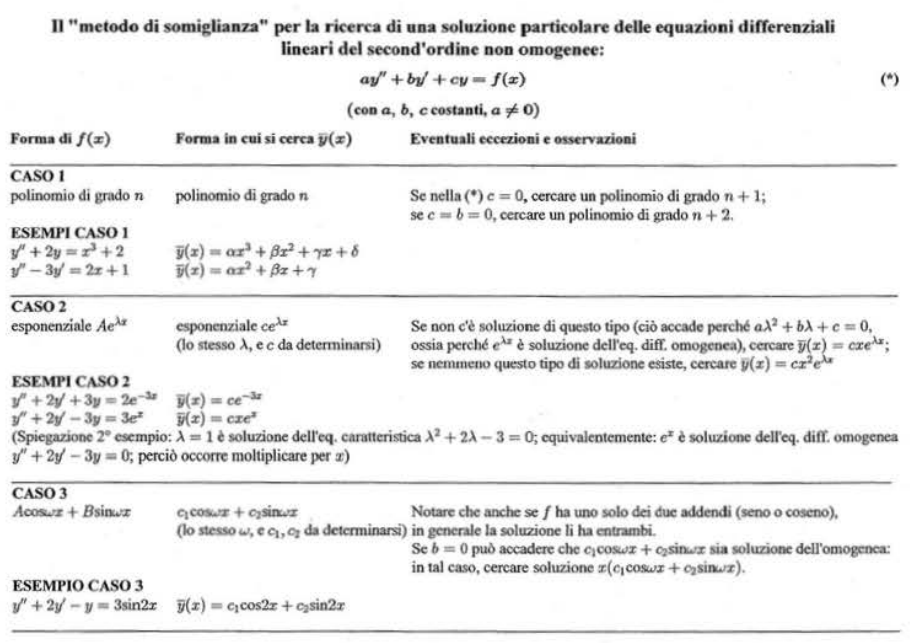
\includegraphics[height=250px]{../img/eqdiff2.PNG}
\end{center}
\begin{center}
    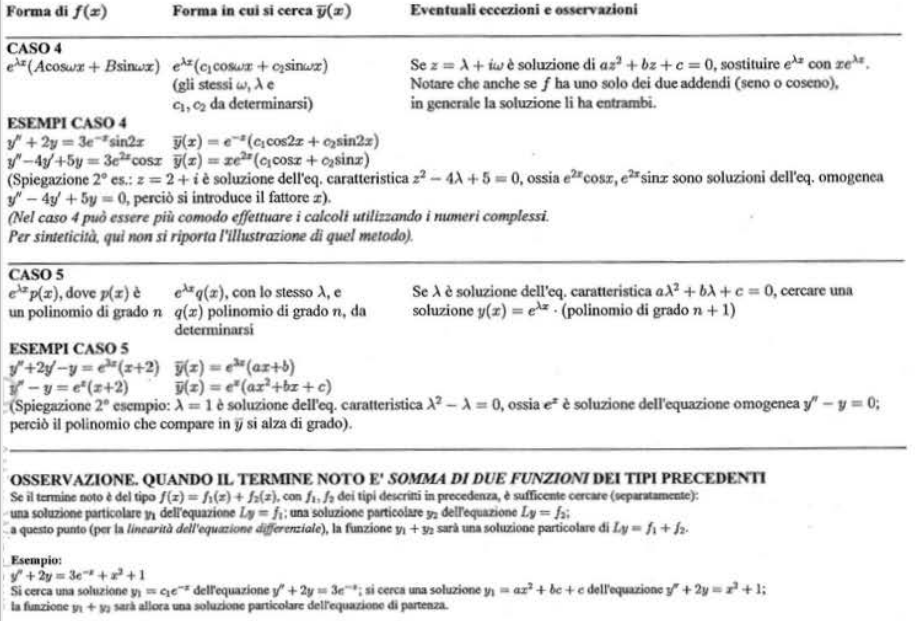
\includegraphics[height=250px]{../img/eqdiff2(1).PNG}
\end{center}
\end{tcolorbox}
\rule{\textwidth}{2pt}
\subsection{Sistemi lineari omogenei}
\[
    y' = A(t) y
\]
viene detto sistema omogeneo.\newline
\[
    \begin{cases}
        y' = A(t) y\\
        y(t_0) = y_0
    \end{cases}
\]
è il problema di cauchy associato.\newline
\newline
Se $y_0 = 0$, allora l'unica soluzione è $y(t) = 0$.\newline
\newline
Se $\phi_1$ e $\phi_2$ risolvono il sistema omogeneo, anche $\alpha \phi_1 + \beta \phi_2$ per ogni $\alpha, \beta \in \mathbb{R}$ lo risolverà.\newline
\newline
Se $A$ è una matrice costante il sistema si dice a coefficienti costanti.\newline
\newline
Sia un matrice $M$, vogliamo calcolare $e^{M}$. \newline
Se $M$ è diagonale si ottiene facilmente:
\[
    M = \left( \begin{matrix}
        \lambda_1  & 0 &\dots & 0\\
        0 & \lambda_2 &\dots &0\\
        0 & 0 &\dots &0\\
        0 & 0 &\dots &\lambda_n
    \end{matrix} \right) \Rightarrow e^M = \left( \begin{matrix}
        e^{\lambda_1}  & 0 &\dots & 0\\
        0 & e^{\lambda_2} &\dots &0\\
        0 & 0 &\dots &0\\
        0 & 0 &\dots & e^{\lambda_n}
    \end{matrix} \right)
\]
Se $M$ non è diagonale, ma è diagonalizzabile, e cioè esiste una matrice non singolare $S$ tale che $\Lambda = S^{-1}MS$ sia diagonale, allora
\[
    M = S\Lambda S^{-1} \Rightarrow  M^k = S\Lambda^kS^{-1} \Rightarrow e^M = S e^{\Lambda}S^{-1}
\]
con $e^{\Lambda}$ che si calcola come abbiamo visto per le matrici diagonali.\newline
\newline
Una matrice quadrata è diagonalizzabile se e solo se tutti i suoi autovalori sono regolari. \newline
\newline
Precisiamo che vengono considerati anche autovalori complessi che, per una matrice a coefficienti reali, possono esserci se e solo se c'è anche il loro coniugato. In tal caso, gli esponenziali dipendenti da tempo vanno interpretati con la formula di Eulero e generano funzioni trigonometriche.\newline
\newline
Abbiamo dunque visto come si trova l'esponenziale di una matrice diagonalizzabile costante. Volendo trovare l'esponenziale della matrice $At$, facciamo un paio di osservazioni elementari:
\begin{itemize}
    \item se A è diagonalizzabile, lo è anche $At$ e si può usare la stessa mtrice di passaggio $S$ per diagonalizzarla
    \item gli autovali di $At$ sono uguali agli autovalori di $A$ moltiplicati per $t$
\end{itemize}
Da queste osservazioni possiamo dedurre che
\[
    e^A  S e^{\Lambda}S^{-1} \Rightarrow  e^{At} = S e^{\Lambda t} S^{-1}
\]
\textbf{teor.} Le colonne della matrice $e^{At}$ formano un sistema fondamentale di soluzioni di $y' = Ay$ e cioè, per ogni $C \in \mathbb{R}^n$ il vettore $e^{At} C$è una soluzione di di $y'=Ay$\newline
\newline
La fuznione $\phi(t) = C e^{\lambda t} $ è soluzione di $y'=At$ se e solo se $\lambda$ è un autovalore di $A$ (possibilmente complesso) e $C$ è un autovettore associato a $\lambda$.\newline
\rule{\textwidth}{0,4pt}
\subsection{Diagonalizzazione di una matrice}
Una matrice $A$ è diagonalizzabile se
\begin{itemize}
    \item Il numero degli autovalori di $A$ contati con la loro molteplicità è uguale all'ordine della matrice
    \item la molteplicità geometrica di ciascun autovalore coincide  con la realtiva molteplicità algebrica
\end{itemize}

Sia $A$ una matrice, i suoi autovalori si ottengono risolvendo
\[
    det(A-\lambda I ) = \left| \begin{matrix}
        a_{11} -\lambda & a_{12}\\
        a_{21} & a_{22} - \lambda
    \end{matrix} \right| = 0
\]
risolvendo questa equazione per $\lambda$ otteniamo i vari autovalori.\newline
La molteplicità algebrica consiste nel quante volte $\lambda$ appare come soluzione dell'equazione precedente.\newline
Perchè $A$ sia diagonalizzabile, la somma della molteplicità algebrica di ogni autovalore deve essere uguale all'ordine della matrice.\newline
Perchè $A$ sia diagonalizzabile bisogna anche verificare che la molteplicità algebrica di ogni autovalore coincide con la realtiva molteplicità geometrica, che si calcola così:
\[
    m_g(\lambda) = n - rk(A- \lambda I)
\]
dove $n$ è l'ordine di $A$.\newline
\newline
\newline
Se $A$ è diagonalizzabile, allora esiste una matrice $P$  che la diagonalizza e una matrice $D$ a cui $A$ è simile, per cui valga:
\[
    D = P A P^{-1}
\]
\begin{itemize}
    \item la matrice $D$ è una matrice diagonale i cui elementi della diagonale principale sono gli autovalori della matrice $A$. Gli autovalori con molteplicità algebrica maggiore di 1 vanno ripetuti più volte.
    \item la matrice $P$ è la matrice che ha come colonne gli autovettori associati a ogni autovalore, ossia ha come colonne i vettori che fromano le basi degli autospazi relativi a ciascun autovalore.
\end{itemize}
Affinchè tutto funzioni ci deve essere corrispondenza fra le matrici $D$ e $P$: la $j$-esima colonna della matrice $P$ contiene l'autovettore associato all'autovalore presente nella $j$-esima colonna della matrice $D$.\newline
\newline
Il calcolo degli autovettori relativi a un autovalore $\lambda$ si esegue risolvendo il sistema:
\[
    (A- \lambda I ) v = 0
\]
con $v = \binom{x}{y}$, e cioè risolvendo il sistema:
\[
    \left(\begin{matrix}
        a_{11} -\lambda & a_{12}\\
        a_{21} & a_{22} - \lambda
    \end{matrix} \right) \binom{x}{y} = 0
\]
\newline
Invece per calcolare l'inversa della matrice $P$ si seguono i seguenti passaggi:
\begin{itemize}
    \item Calcola la trasposta $A^T$ della matrice $A$ (basta scambiare tra loro le righe con le colonne)
    \item sostituire ogni elemento della matrice trasposta col il proprio complemento algebrico (complemento algebrico: preso l'elemento $a_{h,k}$ della matrice, il suo complemento algebrico si calcola come $(-1)^{(h+k)}\cdot C_{h,k}$, dove con $X_{h,k}$ si intende il determinante della matrice ottenuta da quella di partenza eliminando la riga $h$ e la colonna $k$)
    \item Adesso dividi la matrice dei complementi algebrici per det(A) (cioe' dividi ogni termine per det(A)) e ottieni l'inversa della matrice quadrata di partenza
\end{itemize} % equazioni differenziali:
    %- da confrontare con capitolo 7 del libro del prof
    %- aggiugnere capitolo 8 del libro del prof
\end{document}